%% abtex2-modelo-trabalho-academico.tex, v-1.9.2 laurocesar
%% Copyright 2012-2014 by abnTeX2 group at http://abntex2.googlecode.com/ 
%%
%% This work may be distributed and/or modified under the
%% conditions of the LaTeX Project Public License, either version 1.3
%% of this license or (at your option) any later version.
%% The latest version of this license is in
%%   http://www.latex-project.org/lppl.txt
%% and version 1.3 or later is part of all distributions of LaTeX
%% version 2005/12/01 or later.
%%
%% This work has the LPPL maintenance status `maintained'.
%% 
%% The Current Maintainer of this work is the abnTeX2 team, led
%% by Lauro César Araujo. Further information are available on 
%% http://abntex2.googlecode.com/
%%
%% This work consists of the files abntex2-modelo-trabalho-academico.tex,
%% abntex2-modelo-include-comandos and abntex2-modelo-references.bib
%%

% ------------------------------------------------------------------------
% ------------------------------------------------------------------------
% abnTeX2: Modelo de Trabalho Academico (tese de doutorado, dissertacao de
% mestrado e trabalhos monograficos em geral) em conformidade com 
% ABNT NBR 14724:2011: Informacao e documentacao - Trabalhos academicos -
% Apresentacao
% ------------------------------------------------------------------------
% ------------------------------------------------------------------------

\documentclass[
	% -- opções da classe memoir --
	12pt,				% tamanho da fonte
	openright,			% capítulos começam em pág ímpar (insere página vazia caso preciso)
	twoside,			% para impressão em verso e anverso. Oposto a oneside
	a4paper,			% tamanho do papel. 
	% -- opções da classe abntex2 --
	%chapter=TITLE,		% títulos de capítulos convertidos em letras maiúsculas
	%section=TITLE,		% títulos de seções convertidos em letras maiúsculas
	%subsection=TITLE,	% títulos de subseções convertidos em letras maiúsculas
	%subsubsection=TITLE,% títulos de subsubseções convertidos em letras maiúsculas
	% -- opções do pacote babel --
	english,			% idioma adicional para hifenização
	french,				% idioma adicional para hifenização
	spanish,			% idioma adicional para hifenização
	brazil				% o último idioma é o principal do documento
	]{abntex2}

% ---
% Pacotes básicos 
% ---
\usepackage{lmodern}			% Usa a fonte Latin Modern			
\usepackage[T1]{fontenc}		% Selecao de codigos de fonte.
\usepackage[utf8]{inputenc}		% Codificacao do documento (conversão automática dos acentos)
\usepackage{lastpage}			% Usado pela Ficha catalográfica
\usepackage{indentfirst}		% Indenta o primeiro parágrafo de cada seção.
\usepackage{color}				% Controle das cores
\usepackage{graphicx}			% Inclusão de gráficos
\usepackage{microtype} 			% para melhorias de justificação
% ---
		
% ---
% Pacotes adicionais, usados apenas no âmbito do Modelo Canônico do abnteX2
% ---
\usepackage{lipsum}				% para geração de dummy text
\usepackage{amsmath}            % equações matemáticas
\usepackage[section]{placeins}  %manter imagens dentro das seções
% ---

% ---
% Pacotes de citações
% ---
\usepackage[brazilian,hyperpageref]{backref}	 % Paginas com as citações na bibl
\usepackage[alf]{abntex2cite}	% Citações padrão ABNT

% ---
% Pacotes adicionados por Roberto Rolo
% ---
\usepackage{verbatim}	              %usado para comentar blocos
\usepackage{subfig}                   %usado para colocar figuras lado a lado
\usepackage{tabularx}                 %usado para forçar tabelas a ocupar a largura do texto
\usepackage[section]{placeins}  %não deixa imagens ultrapassarem barreira
%\usepackage{upgreek}                  %letras gregas
\usepackage{float}               %força posição das imagens
\usepackage{url}                %links com underline


%check boxes

\usepackage{enumitem,amssymb}
\newlist{todolist}{itemize}{2}
\setlist[todolist]{label=$\square$}
\usepackage{pifont}
\newcommand{\cmark}{\ding{51}}%
\newcommand{\xmark}{\ding{55}}%
\newcommand{\done}{\rlap{$\square$}{\raisebox{2pt}{\large\hspace{1pt}\cmark}}%
	\hspace{-2.5pt}}
\newcommand{\wontfix}{\rlap{$\square$}{\large\hspace{1pt}\xmark}}

% --- 
% CONFIGURAÇÕES DE PACOTES
% --- 

% ---
% Configurações do pacote backref
% Usado sem a opção hyperpageref de backref
\renewcommand{\backrefpagesname}{Citado na(s) página(s):~}
% Texto padrão antes do número das páginas
\renewcommand{\backref}{}
% Define os textos da citação
\renewcommand*{\backrefalt}[4]{
	\ifcase #1 %
		Nenhuma citação no texto.%
	\or
		Citado na página #2.%
	\else
		Citado #1 vezes nas páginas #2.%
	\fi}%
% ---

% ---
% Informações de dados para CAPA e FOLHA DE ROSTO
% ---
\titulo{Aprimoramentos em modelagem geológica implícita com funções distância assinaladas \\~\\ \small{Proposta de tese para o exame de qualificação}}
\autor{Roberto Mentzingen Rolo}
\local{Porto Alegre}
\data{2018}
\orientador{João Felipe Coimbra Leite Costa}
%\coorientador{Equipe \abnTeX}
\instituicao{%
  Universidade Federal do Rio Grande do Sul - UFRGS
  \par
  Faculdade de Engenharia
  \par
  Programa de Pós-Graduação em Engenharia de Minas, Metalúrgica e de Materiais}
\tipotrabalho{Proposta de tese para o exame de qualificação}
% O preambulo deve conter o tipo do trabalho, o objetivo, 
% o nome da instituição e a área de concentração 
\preambulo{preambulo}
% ---


% ---
% Configurações de aparência do PDF final

% alterando o aspecto da cor azul
\definecolor{blue}{RGB}{41,5,195}

% informações do PDF
\makeatletter
\hypersetup{
     	%pagebackref=true,
		pdftitle={\@title}, 
		pdfauthor={\@author},
    	pdfsubject={\imprimirpreambulo},
	    pdfcreator={LaTeX with abnTeX2},
		pdfkeywords={abnt}{latex}{abntex}{abntex2}{trabalho acadêmico}, 
		colorlinks=true,       		% false: boxed links; true: colored links
    	linkcolor=blue,          	% color of internal links
    	citecolor=blue,        		% color of links to bibliography
    	filecolor=magenta,      		% color of file links
		urlcolor=blue,
		bookmarksdepth=4
}
\makeatother
% --- 

% --- 
% Espaçamentos entre linhas e parágrafos 
% --- 

% O tamanho do parágrafo é dado por:
\setlength{\parindent}{1.3cm}

% Controle do espaçamento entre um parágrafo e outro:
\setlength{\parskip}{0.2cm}  % tente também \onelineskip

% ---
% compila o indice
% ---
\makeindex
% ---

% ----
% Início do documento
% ----
\begin{document}

% Retira espaço extra obsoleto entre as frases.
\frenchspacing 

% ----------------------------------------------------------
% ELEMENTOS PRÉ-TEXTUAIS
% ----------------------------------------------------------
% \pretextual

% ---
% Capa
% ---
\imprimircapa
% ---

% ---
% Folha de rosto
% (o * indica que haverá a ficha bibliográfica)
% ---
%\imprimirfolhaderosto*
% ---

% ---
% inserir lista de ilustrações
% ---
\pdfbookmark[0]{\listfigurename}{lof}
\listoffigures*
\cleardoublepage
% ---

\begin{comment}
% ---
% inserir lista de tabelas
% ---
\pdfbookmark[0]{\listtablename}{lot}
\listoftables*
\cleardoublepage
% ---

% ---
% inserir lista de abreviaturas e siglas
% ---
\begin{siglas}
  \item[ABNT] Associação Brasileira de Normas Técnicas
  \item[abnTeX] ABsurdas Normas para TeX
\end{siglas}
% ---

% ---
% inserir lista de símbolos
% ---
\begin{simbolos}
  \item[$ \Gamma $] Letra grega Gama
  \item[$ \Lambda $] Lambda
  \item[$ \zeta $] Letra grega minúscula zeta
  \item[$ \in $] Pertence
\end{simbolos}
% ---
\end{comment}

% ---
% inserir o sumario
% ---
\pdfbookmark[0]{\contentsname}{toc}
\tableofcontents*
\cleardoublepage
% ---



% ----------------------------------------------------------
% ELEMENTOS TEXTUAIS
% ----------------------------------------------------------
\textual

\chapter{Introdução}

Estimativas de recursos e reservas minerais demandam a construção de modelos numéricos de teores de longo prazo, que abrangem toda a extensão do depósito mineral e compreendem todo o tempo de vida da mina. Esses modelos são atualizados em intervalos de um a três anos de operação. Modelos de médio prazo podem ser construídos para planejar de um a seis meses no futuro do empreendimento. Enquanto modelos de curto prazo, são construídos com o objetivo de balizar, semanalmente ou diariamente, as decisões relativas a controle de teores e planejamento detalhado da mina.

Construir modelos numéricos de longo, médio e curto prazo para avaliação de recursos/reservas e planejamento de mina exige quatro grandes atividades \cite{rossi2013mineral}:

\begin{enumerate}
\item Coleta e gerenciamento de dados;
\item Interpretação e modelagem geológica;
\item Atribuição de teores;
\item Avaliação e gerenciamento da incerteza geológica e de teores.
\end{enumerate}

Após a coleta, gerenciamento e checagem dos dados, é necessário identificar diferentes domínios. A determinação dos domínios deve ser baseada no conhecimento geológico, i.e. zonas de oxidação, litologias, alteração ou limites estruturais e deve ser suportada por extensiva análise estatística (análise exploratória dos dados), incluindo análises variográficas. É importante que a definição dos domínios faça sentido espacial e geológico. Os domínios são, algumas vezes, baseados na combinação de duas ou mais variáveis para as quais a correlação entre os teores pode ser demonstrada. O procedimento pode ser bastante demorado, principalmente em depósitos multivariados, entretanto, as estimativas são melhoradas significativamente quando cuidadosamente limitadas por variáveis geológicas \cite{rossi2013mineral}.

A definição de diferentes domínios de estimativas, ou zonas estacionárias no interior do depósito, é necessária porque a inferência geoestatística, geralmente, o método de escolha para a construção dos modelos numéricos de teores, exige decisão de estacionariedade \cite{mclennanstationarity}. Isto é, os teores em cada domínio estacionário pertencem a populações estatísticas distintas, são caracterizados através de modelos de distribuição e de covariância específicos e devem ser modelados como funções aleatórias estacionárias diferentes. \cite{journel1978mining}. 

Uma função aleatória estacionária é uma representação probabilística de uma propriedade petrofísica com valor esperado e covariância constantes independente da localização \cite{mclennanstationarity}. Estacionariedade, definida por \citeonline{matheron1962traite}, é uma propriedade do modelo de função aleatória, não é uma característica intrínseca da variável. É uma decisão tomada pelo geomodelador e necessária para a inferência.

Os domínios estacionários não devem ser muito pequenos, dessa forma não existirão dados suficientes para descrição e inferência estatística confiável, e nem muito grandes, já que os dados, provavelmente, poderiam ser subdivididos em grupos geologicamente mais homogêneos. A definição adequada dos domínios estacionários é uma etapa importante na avaliação de recursos/reservas, a mistura de populações produz estimativas sub ótimas que superestimam ou subestimam teores e tonelagens. Além disso, nenhuma técnica geoestatística pode compensar uma definição de estacionariedade inadequada \cite{rossi2013mineral}.

Uma vez que os domínios estacionários tenham sido definidos, um modelo tridimensional que defina os limites de cada função aleatória estacionária deve ser construído: o modelo geológico. É necessário identificar a "jurisdição espacial" de cada função aleatória estacionária. Inevitavelmente, existe incerteza associada à localização dos limites, e essa incerteza geológica deve ser quantificada \cite{mclennanstationarity}. A etapa de Interpretação e modelagem geológica compreende a definição dos domínios estacionários e a criação do modelo geológico tridimensional que forma o alicerce para todo o trabalho de estimativa subsequente. Muitas vezes, o modelo geológico é o fator de maior importância na estimativas das tonelagens mineralizadas \cite{rossi2013mineral}.

A abordagem tradicional para a criação de modelos geológicos tridimensionais é através da triangulação de polilinhas \footnote{Em computação gráfica: uma linha composta por vários segmentos, usada para compor imagens na tela \cite{oxfordonlinedictionary}.} (\textit{strings}) gerando sólidos que representam os corpos minerais. As polilinhas são digitalizadas manualmente em seções deslocadas, a partir dos dados de sondagem e conhecimento geológico prévio, por um geomodelador. As seções são unidas por linhas guias, que demarcam a conectividade entre as seções digitalizadas para triangulação adequada dos sólidos. Esse procedimento é referido como modelagem geológica explícita, já que a os limites entre os diferentes domínios são definidos explicitamente por coordenadas (x,y,z) que posicionam a "colcha de retalhos" de triângulos \cite{mclennan2006boundsim,cowan2003practical}. A \autoref{explicitmodeling} ilustra a metodologia explícita para um típico depósito de veio.

\begin{figure}[!htb]
	\caption{\label{explicitmodeling}Ilustração esquematizando a modelagem geológica explícita usando polilinhas e linhas guias.}
	\begin{center}
		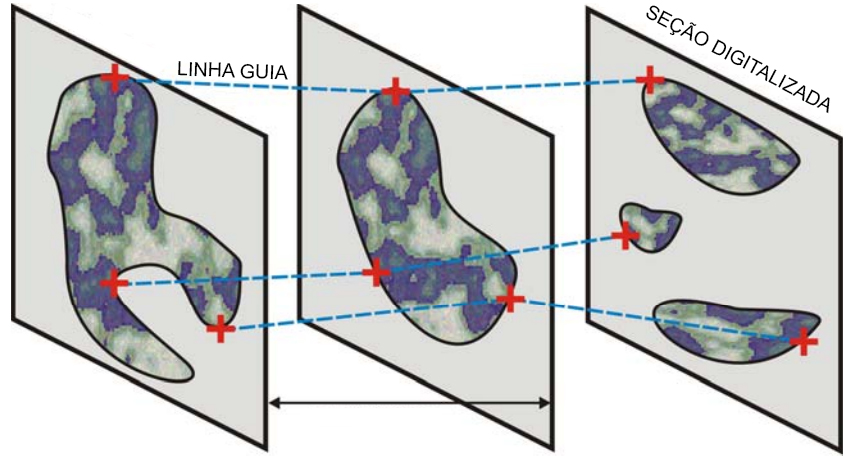
\includegraphics[width=0.6\textwidth]{capitulo_1/explicitmodeling}
	\end{center}
	\legend{Modificado de \citeonline{mclennan2006boundsim}}
\end{figure}

De acordo com \citeonline{mclennan2006boundsim}, embora a metodologia seja direta e simples, principais motivos da sua ampla implementação na prática, e que \textit{softwares} modernos de mineração forneçam ferramentas computais para visualizar os dados de sondagem e agilizar o processo de digitalização \cite{silvaenhancedgeomodeling}, existem uma série de limitações e desvantagens. O processo é tedioso e demorado, digitalizar manualmente as polilinhas e uni-las por linhas guia, exige muito tempo de um profissional experiente. Em depósitos de alta complexidade, não é raro o geomodelador trabalhar até três meses no modelo geológico explícito. A geometria dos corpos geológicos muitas vezes precisa ser simplificadas para que o modelo seja concebido em tempo hábil. Por esse motivo, para a maioria das minas, apenas um modelo é construído e mantido, raramente há oportunidade de modelar interpretações geológicas alternativas e comparar estimativas de recursos baseadas em diferentes modelos \cite{cowan2003practical}.

Os modelos criados explicitamente são subjetivos e não replicáveis. O volume mineralizado é essencialmente composto por por uma série de pequenas decisões subjetivas, já que cada ponto da polilinha em cada seção é escolhido por um geomodelador. Inevitavelmente, a "assinatura" do profissional é impressa nos limites dos domínios geológicos. Geomodeladores diferentes criam modelos diferentes a partir do mesmo banco de dados. Ademais, modelos explícitos são inflexíveis, é laborioso e demorado atualizar modelos explícitos a medida que novos dados são obtidos já que uma nova digitalização manual é necessária.

Em virtude da onerosidade em construir múltiplos modelos geológicos explícitos, é custoso avaliar a incerteza na localização dos limites dos diferentes domínios entre os dados amostrais, como mostrado na ilustração esquemática na \autoref{incerteza_limites}. Além da tediosa redigitalização manual de polilinhas e retriangulação, não existe forma direta de incorporar múltiplas realizações possíveis para a localização dos limites que representam a incerteza associada.

\begin{figure}[!htb]
	\caption{\label{incerteza_limites}Ilustração esquemática destacando a incerteza na localização do limite entre os domínios azul e vermelho, entre os dados amostrais.}
	\begin{center}
		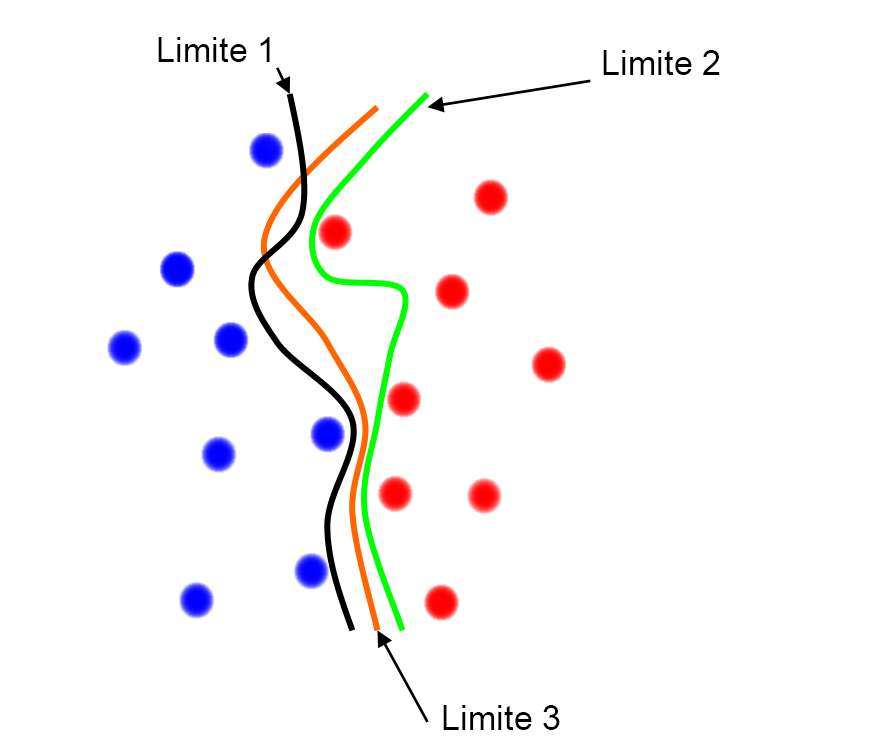
\includegraphics[width=0.6\textwidth]{capitulo_1/incerteza_limites}
	\end{center}
	\legend{Modificado de \citeonline{caceres2011stochastic}}
\end{figure}

Em muitos casos, a incerteza do modelo geológico pode ser uma fonte de incerteza crucial. Em depósitos de veio de ouro, por exemplo, o volume mineralizado é um indicador econômico vital para o gerenciamento do projeto. Ignorar a incerteza volumétrica, considerando apenas um único modelo geológico explícito, pode ser ser devastador para o empreendimento. A incerteza associada ao modelo geológico deve ser avaliada.

Embora a metodologia explícita seja demorada, laboriosa, subjetiva, não replicável, inflexível e incapaz de avaliar incertezas, o limites entre domínios resultantes, geralmente, são realistas. Realismo geológico é um dos principais objetivos da modelagem e pode ser diretamente controlado durante o processo de digitalização. 

Dadas as desvantagens do método explícito de modelagem geológica, pesquisas vêm sendo realizadas com o objetivo de automatizar, ou pelo menos, semi automatizar a modelagem. Métodos matemáticos menos sofisticados, como o vizinho mais próximo podem ser utilizados na criação automática de modelos geológicos determinísticos.  Métodos geoestatísticos também têm aplicação, a krigagem dos indicadores, \cite{journel1982indicator} consiste na geração de uma distribuição acumulada de probabilidades a partir da transformação não linear dos dados. Para variáveis categóricas, é possível estimar diretamente a probabilidade de cada local não amostrado pertencer à cada uma das diferentes litologias do depósito mineral.

A necessidade de avaliação da incerteza associada ao modelo geológico impulsionou o desenvolvimento de métodos estocásticos baseados em múltiplas realizações equiprováveis de um atributo. A partir da análise conjunta das realizações é possível avaliar a incerteza. 

São metodologias estabelecidas da geoestatística clássica, baseada no variograma: a simulação sequencial dos indicadores \cite{goovaerts1997geostatistics}, que compartilha do mesmo princípio da krigagem dos indicadores. A simulação gaussiana truncada \cite{matheron1987conditional}, que tem como ideia central gerar múltiplas realizações de uma variável aleatória gaussiana contínua e truncá-las em uma série de limites pré definidos, indicando as diferentes litologias. A simulação plurigaussiana truncada, \cite{galli1994pros} que é uma extensão da simulação gaussiana truncada, baseada na truncagem de duas funções aleatórias gaussianas que podem ou não ser correlacionadas.

Outras metodologias não baseadas em variograma foram desenvolvidas: a simulação geoestatística multiponto \cite{strebellesimulationscomplexgeology}, tem o mesmo formalismo das simulações sequenciais baseadas em variograma, com a diferença que a distribuição local de probabilidade é encontrada a partir da amostragem de uma imagem de treinamento com um modelo multi ponto \cite{pyrcz2014geostatistical}. Do mesmo modo, a simulação baseada em objetos \cite{alabert1992stochastic, bratvold1995storm, holden1998modeling}, metodologia que produz modelos atrativos (visualmente limpos) que honram a geometria idealizada interpretada a partir de afloramentos ou dados de sísmica. Quando geometrias específicas do depósito ou reservatório são identificadas de forma correta, parametrizadas e têm significância para a função de transferência, podem ser integradas diretamente no modelo pelos métodos baseados em objetos \cite{pyrcz2005stochastic}. 

Uma outra família de métodos, ditos métodos implícitos, compreendem técnicas importadas da computação gráfica. O uso da modelagem implícita foi introduzida no campo da computação gráfica para a geração de objetos de diferentes geometrias e complexidades por  \citeonline{bloomenthal1997introduction}. A ideia geral é usar uma função implícita para demarcar regiões de diferentes formas e extensões no espaço. \citeonline{cowan2002rapid,cowan2003practical} popularizou a modelagem implícita no contexto geológico, baseado no trabalho de \citeonline{savchenko} que modela objetos tridimensionais a partir de dados esparsos interpolando uma função volume (\autoref{busto}).

\begin{figure}[!htb]
	\caption{\label{busto}Busto reconstruído a partir de pontos esparsos.} 
	\begin{center}
		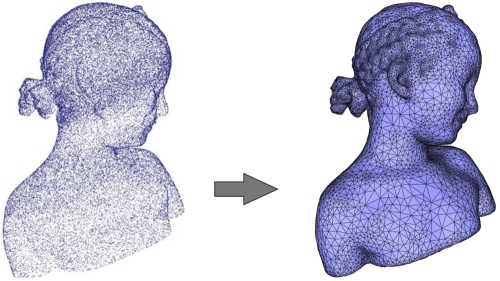
\includegraphics[width=0.6\textwidth]{capitulo_1/busto}
	\end{center}
	\legend{Fonte: \citeonline{poisson_recon}}
\end{figure}

Modelos geológicos implícitos são criados a partir de dados esparsos, geralmente, dados categóricos (\autoref{imp_mod} (a)). Os pontos amostrais podem ser usados para derivar uma função implícita que fornece uma representação matemática contínua de um atributo através de um volume, um campo escalar ou modelo implícito (\autoref{imp_mod} (b)). Modelos implícitos contém um número infinito de isosuperfícies, para visualizar o modelo geológico uma isosuperfície específica deve ser extraída do modelo e mostrada no espaço tridimensional (geralmente a isosuperfície zero), $f(x,y,z)=s$, onde $s$ é o valor de interesse no campo escalar (\autoref{imp_mod} (c)). A localização dessa superfície é conhecida implicitamente como função da localização no domínio \cite{martin2017implicitmodeling}. 

\begin{figure}[!htb]
	\caption{\label{imp_mod}Ilustração esquemática da modelagem geológica implícita.}
	\begin{center}
		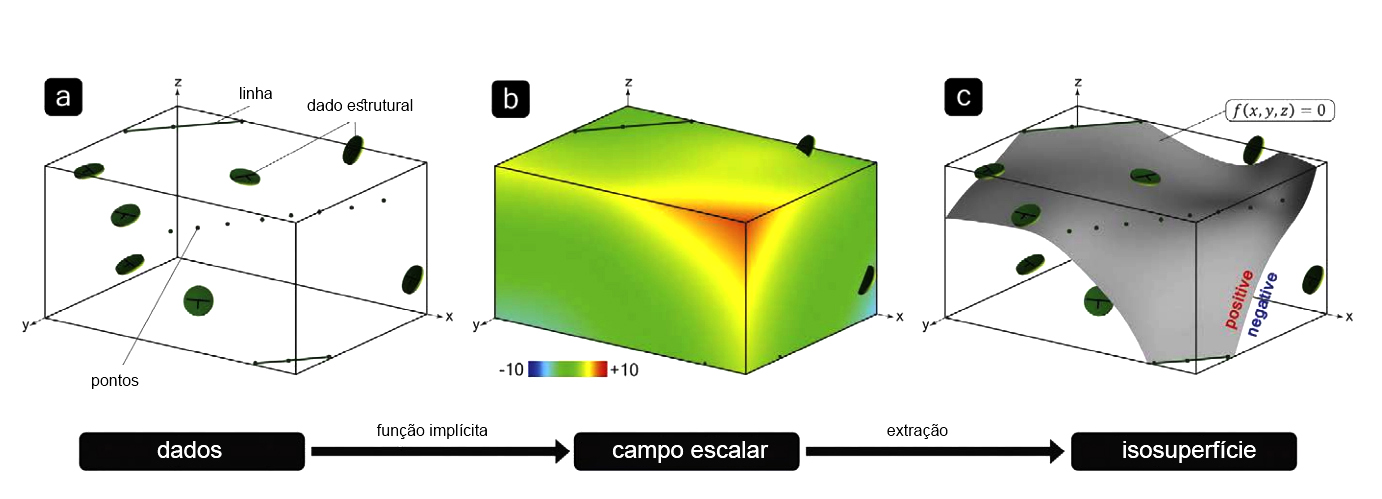
\includegraphics[width=\textwidth]{capitulo_1/implicit_modelig_pt_1}
	\end{center}
	\legend{Modificado de \cite{aillerespresentation}}
\end{figure}

Diferentes tipos de dados amostras podem ser usados para derivar diferentes funções volume na modelagem implícita. \citeonline{mallet2004space} propõe uma função volumétrica cronológica, levando em consideração a posição estratigráfica das diferentes unidades geológicas, enquanto \citeonline{lajaunie1997foliation} usam co-krigagem de incrementos em um campo potencial, omitindo a função volume. A função volume mais comumente utilizada é a função distância assinalada \cite{osherlevelsetmethods}, a aplicação dessa metodologia é encontrada por toda a literatura de interpolação de dados esparsos, uma das aplicações é a reconstrução de superfícies a partir de escaneamento (\autoref{busto}). Na modelagem geológica a metodologia é competente em capturar a geometria e extensão de corpos geológicos e tem sido aplicada com sucesso há mais de 10 anos na exploração mineral tendo ganhado espaço em softwares comerciais como o \textit{Leapfrog \textsuperscript{\textregistered}}. Para bancos de dados pontuais, que representam a posição espacial de diferentes litologias no espaço, o uso das funções distância assinaladas torna os processos de interpretação, cálculo, modelagem, modificação do modelo de acordo com a interpretação dos geomodeladores e avaliação da incerteza diretos e rápidos. Além disso, informações a respeito da orientação das unidades geológicas (dados estruturais) pode ser imputada como restrição na criação do modelo geológico \cite{martin2017implicitmodeling}.
\chapter{Estado da arte} \label{capitulo_2}

Esse capítulo detalha a modelagem geológica implícita com funções distância assinaladas, desde o cálculo das distâncias até a avaliação de incerteza dos modelos geológicos.

O fluxo de trabalho e os diferentes métodos disponíveis na literatura serão apresentados com exemplos práticos em um banco de dados tridimensional sintético que emula um depósito de cobre pórfiro. Pode ser encontrado na íntegra, com toda a memória de cálculo \href{https://drive.google.com/open?id=1JLRrOtOzDVCEpqnG8Ik95xws7Dw6MBvJ}{no repositório}

\section{O banco de dados}

O banco de dados categóricos contém 72 furos totalizando 3349 amostras distribuídas entre 3 diferentes categorias conforme o histograma da \autoref{hist_geo}.

\begin{figure}[H]
	\caption{\label{hist_geo}Histograma do banco de dados.}
	\begin{center}
		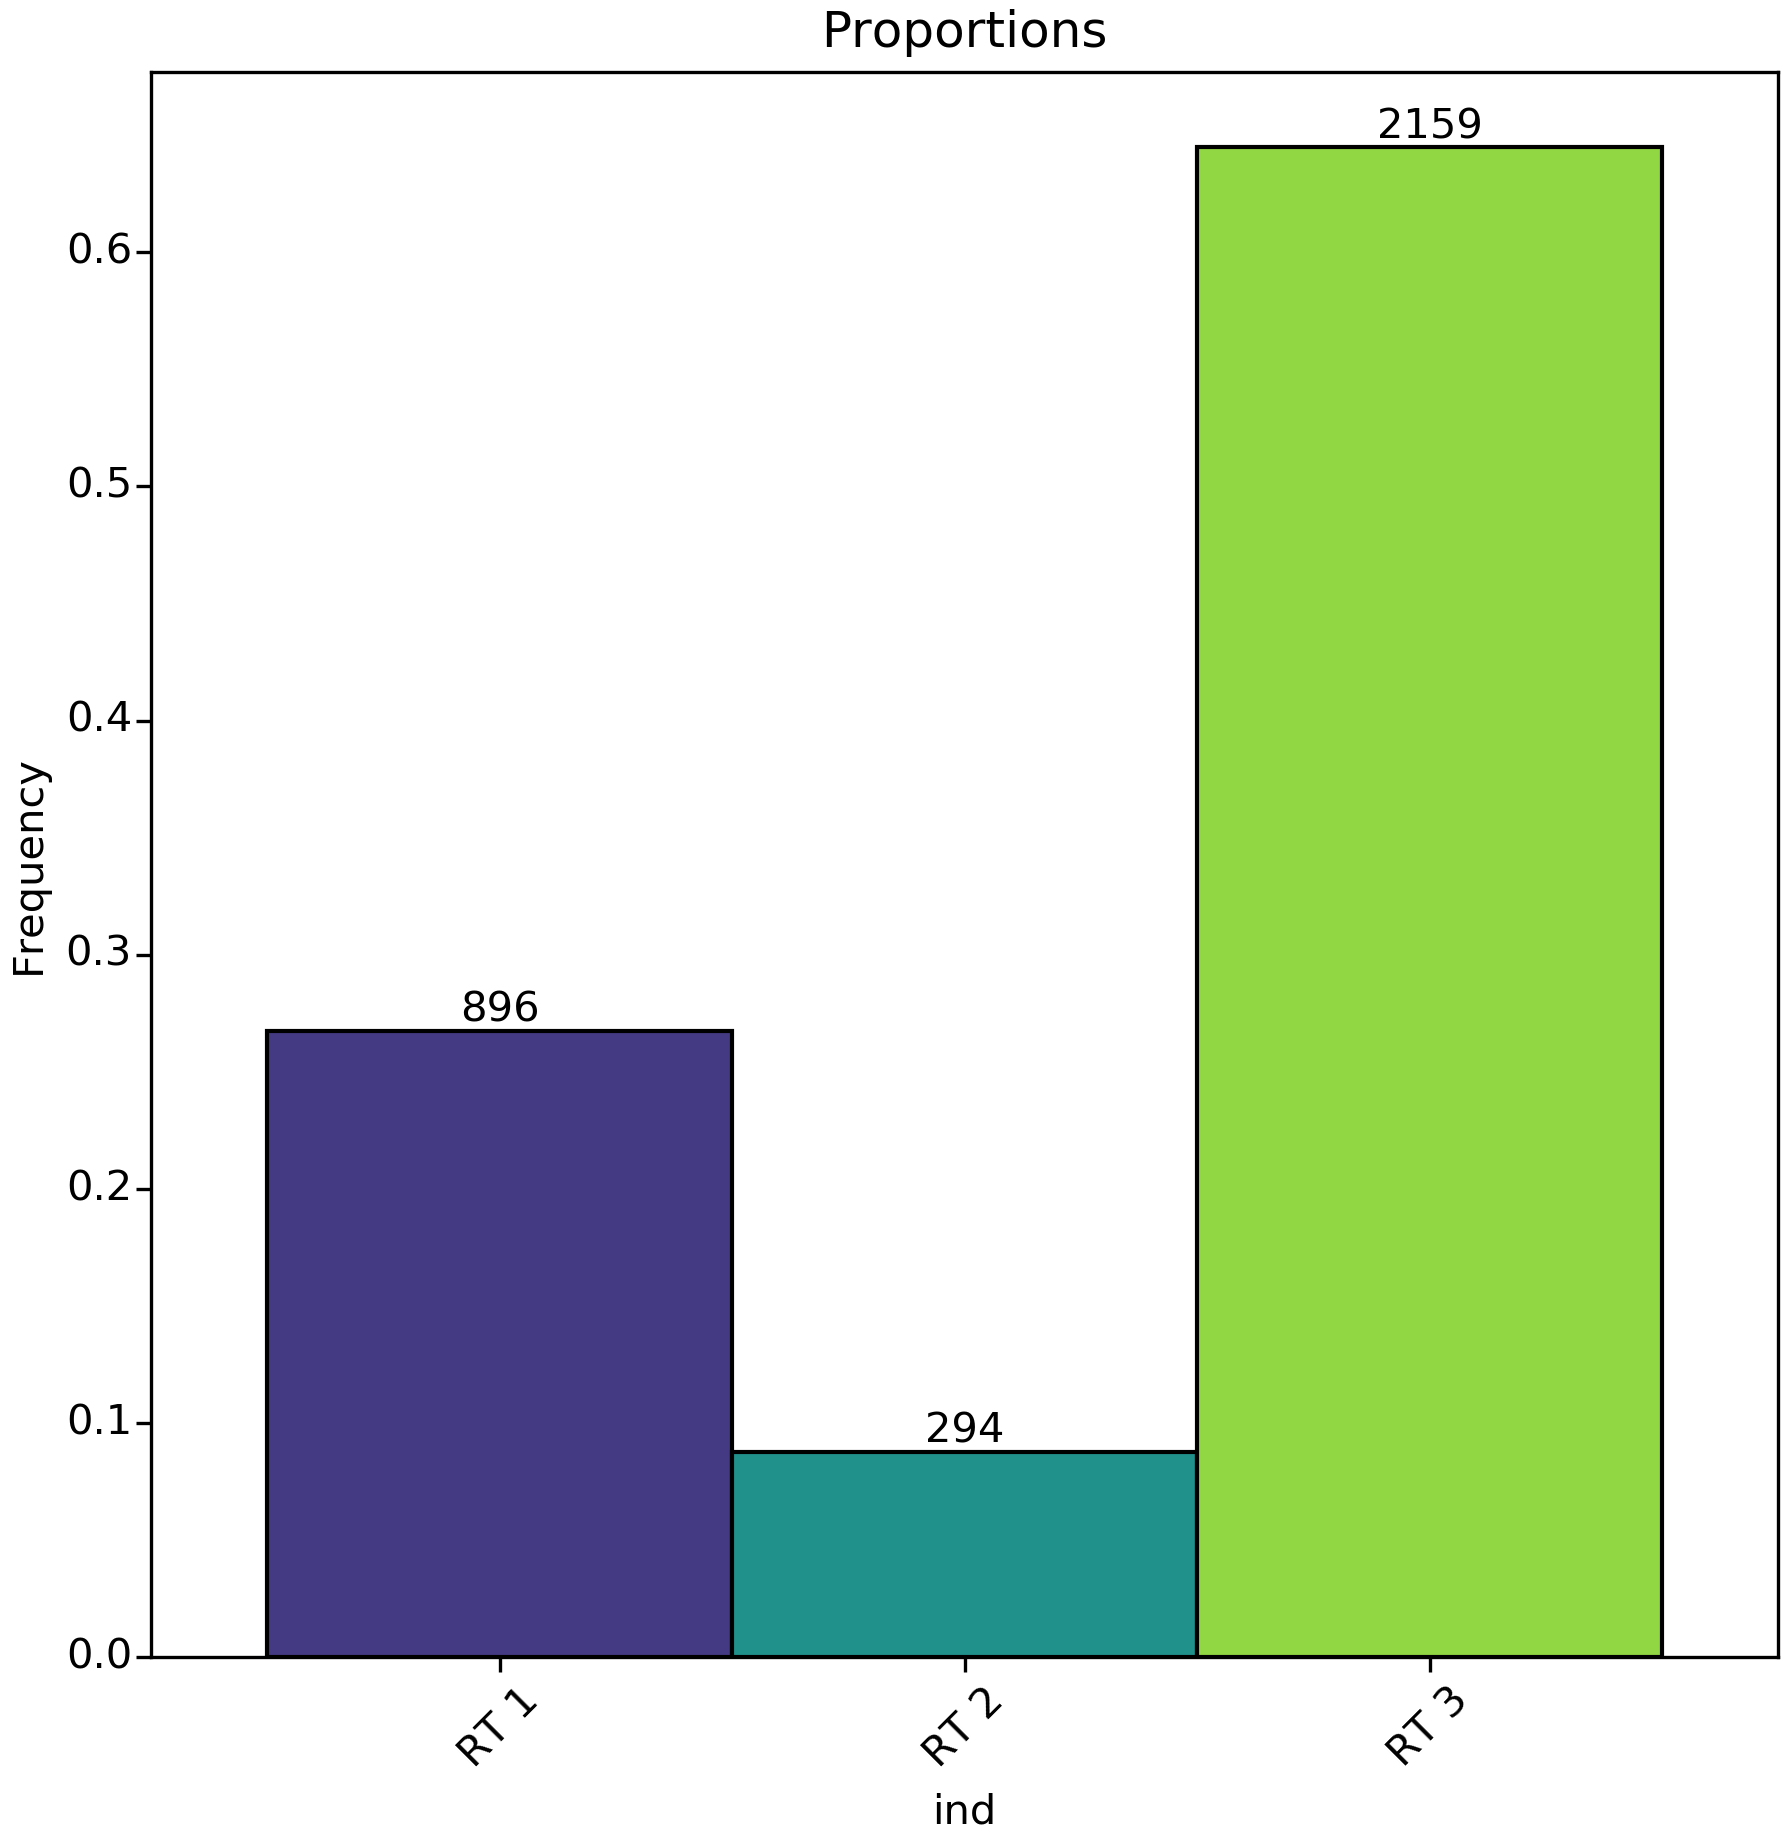
\includegraphics[width=0.5\textwidth]{capitulo_2/prop_hist_big.png}
	\end{center}
	%\legend{Modificado de \citeonline{martin2017implicitmodeling}}
\end{figure}

A \autoref{dataset} mostra a posição espacial das amostras do banco de dados tridimensional.

\begin{figure}[H]
	\caption{\label{dataset}Vista das amostras em perspectiva.}
	\begin{center}
		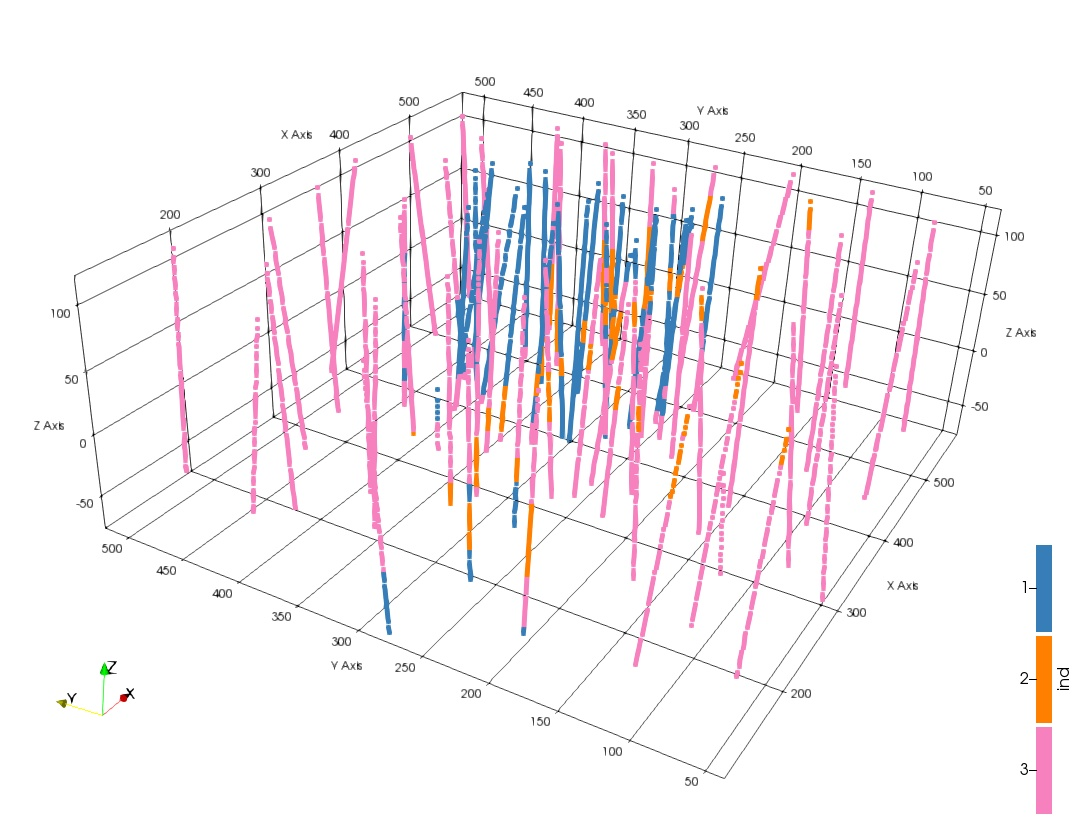
\includegraphics[width=0.8\textwidth]{capitulo_2/dados.jpeg}
	\end{center}
	%\legend{Modificado de \citeonline{martin2017implicitmodeling}}
\end{figure}

\section{A função distância assinalada}

A modelagem implícita é geralmente aplicada à variáveis categóricas que representam diferentes litologias do depósito mineral para definir a localização, extensão e geometria dos corpos minerais. A variável de indicadores deve ser codificada em uma função volumétrica e interpolada exaustivamente para todos os locais de interesse. A função distância assinalada \cite{osherlevelsetmethods}  é a função volume mais utilizada na modelagem implícita de variáveis categóricas.

\subsection{Calculando a função distância assinalada}

O primeiro passo no cálculo das distâncias assinaladas é transformar as amostras ${z(u_\alpha),\alpha=1,...,n}$ em indicadores binários de acordo com a \autoref{eq_ind}, especificando se a amostra pertence ou não ao domínio $k$ que está sendo modelado.

\begin{equation}
	i_k(u_\alpha)=\begin{cases}
	1,\:\textrm{se}\:z(u_\alpha)\:\textrm{se pertence ao domínio $k$}\\
	0,\:\textrm{se}\:z(u_\alpha)\:\textrm{caso contrário}\end{cases}
    \label{eq_ind}
\end{equation}

A \autoref{ind} mostra as amostras codificadas em indicadores para cada uma das três categorias do banco de dados.

\begin{figure}[H]
    \caption{Amostras codificadas em indicadores para cada uma das três categorias do banco de dados.} \label{ind}
     \centering
     \subfloat[][Categoria 1]{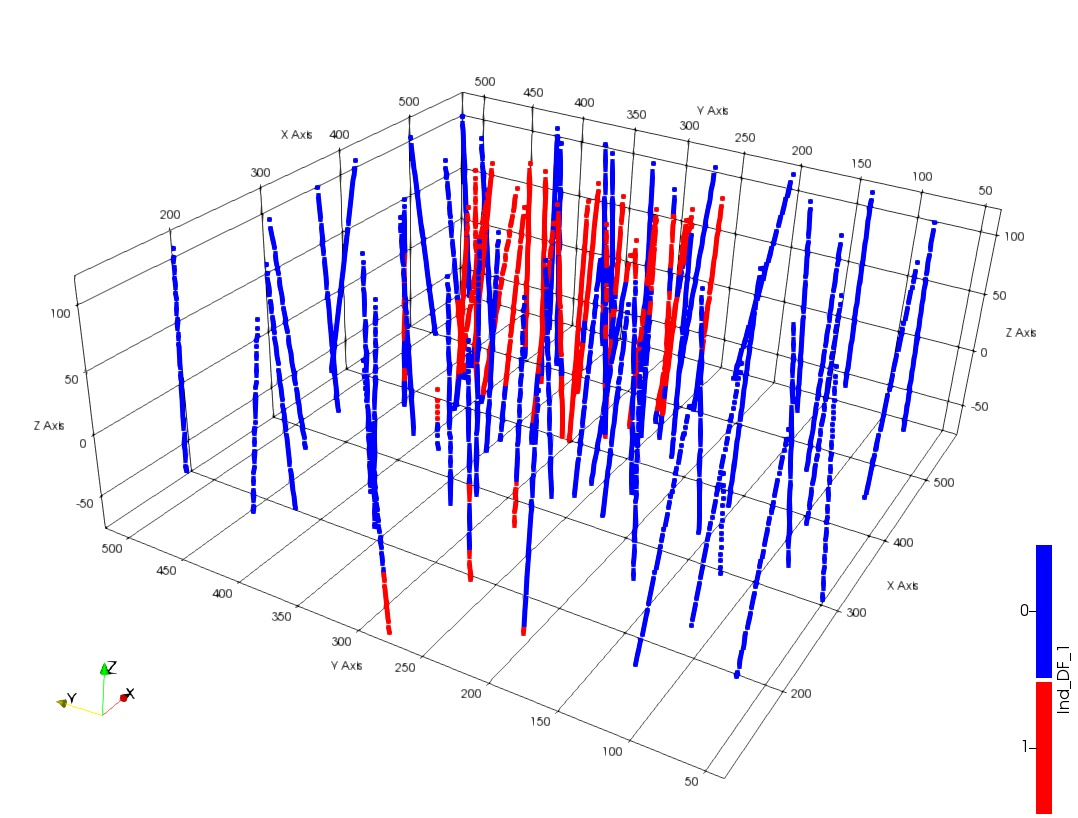
\includegraphics[width=.3\textwidth]{capitulo_2/inddf1.jpeg}\label{<figure1>}}
     \subfloat[][Categoria 2]{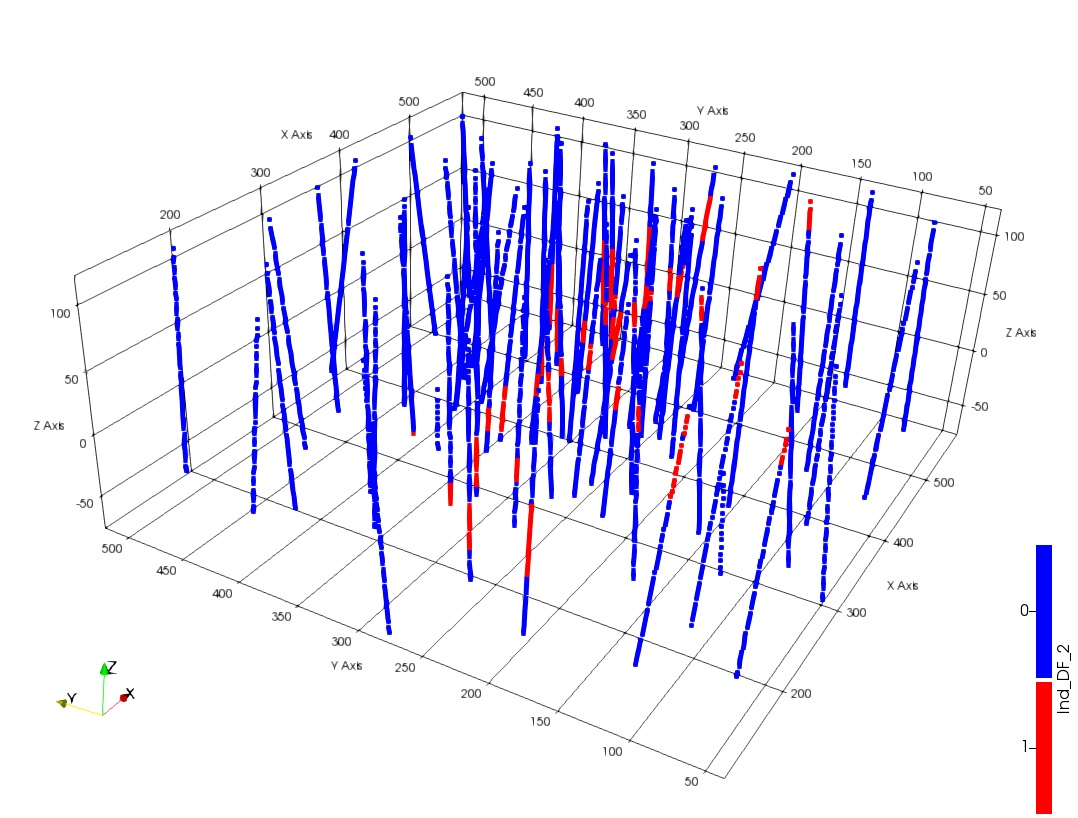
\includegraphics[width=.3\textwidth]{capitulo_2/inddf2.jpeg}\label{<figure2>}}
     \subfloat[][Categoria 3]{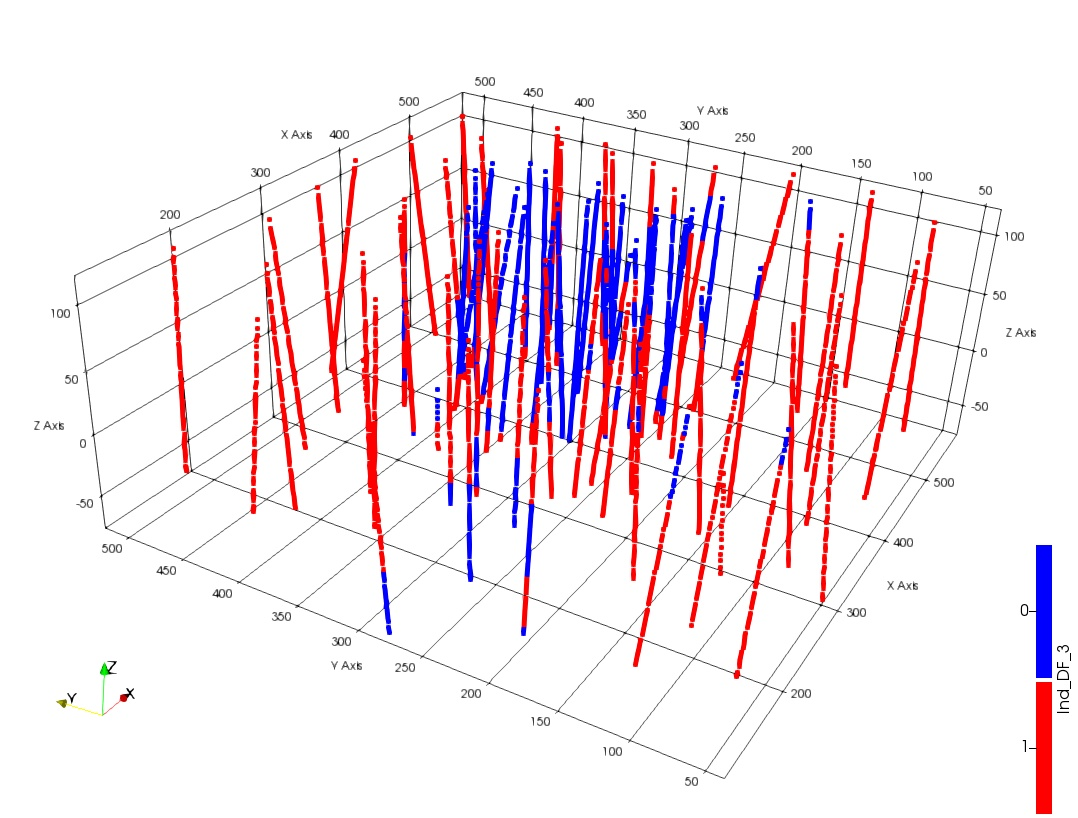
\includegraphics[width=.3\textwidth]{capitulo_2/inddf3.jpeg}\label{<figure2>}}
\end{figure}

O segundo passo é o cálculo das distâncias assinaladas. Para cada ponto amostral, a menor distância euclideana até um outro ponto amostral que pertence à um indicador oposto é computada, e esse valor atribuído àquele ponto, com o sinal negativo caso pertença ao domínio modelado e com o sinal positivo, caso contrário como ilustrado na \autoref{2d_ex}. 

\begin{figure}[H]
	\caption{\label{2d_ex}Ilustração esquemática mostrando o cálculo das distâncias assinaladas.}
	\begin{center}
		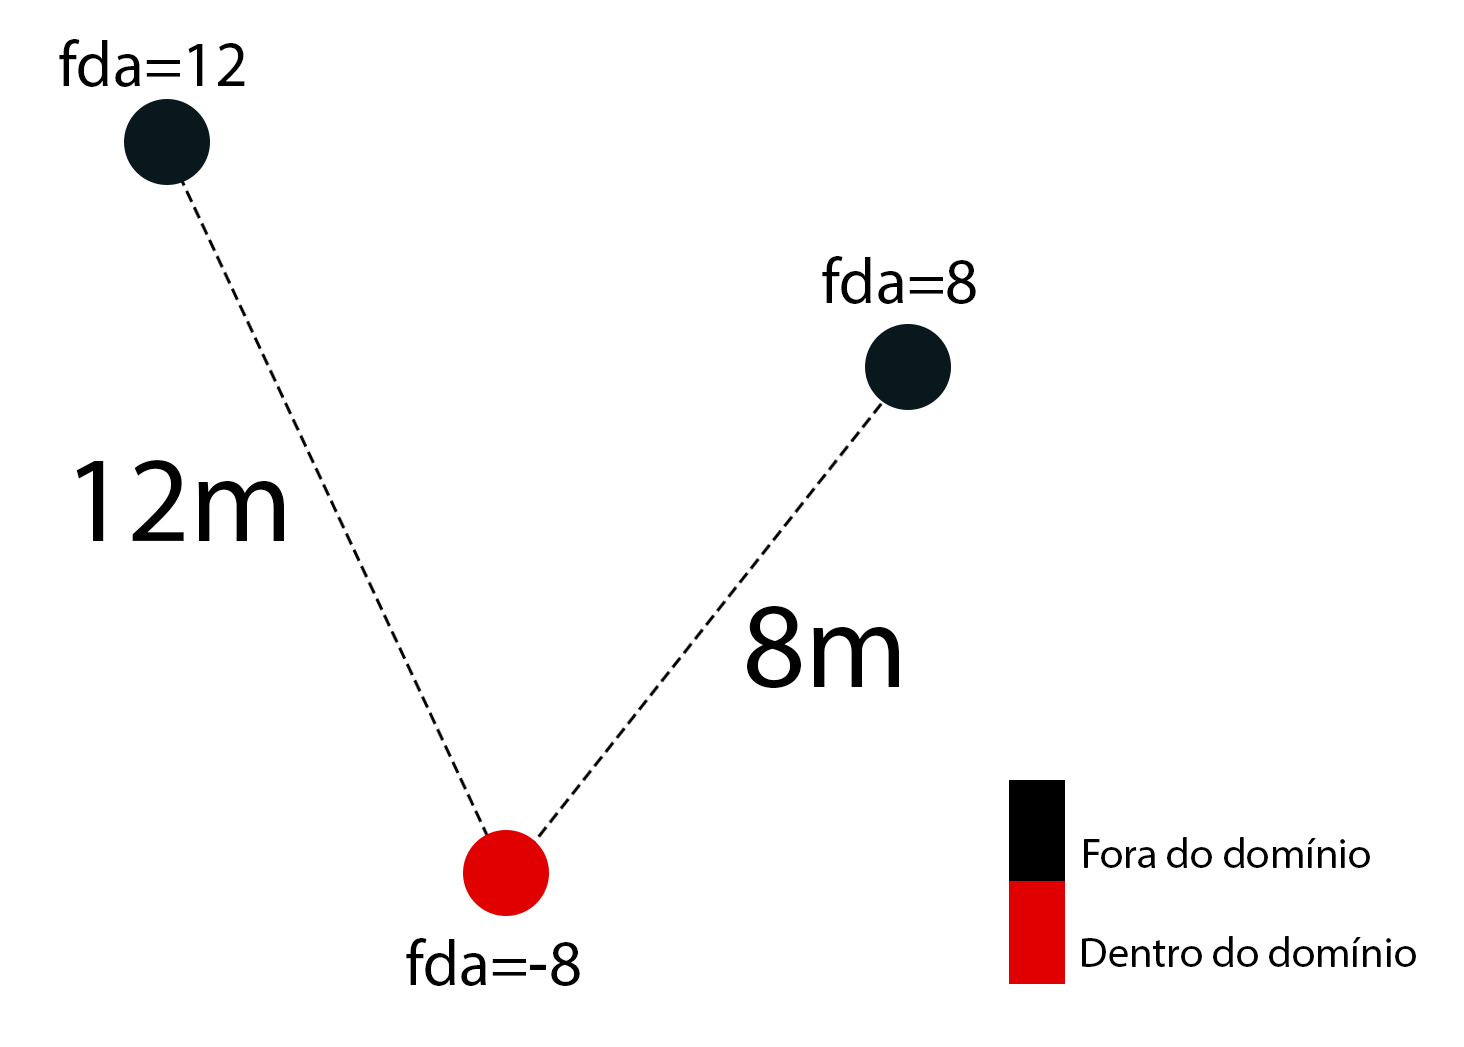
\includegraphics[width=0.6\textwidth]{capitulo_2/2d_ex.jpg}
	\end{center}
	%\legend{Modificado de \citeonline{martin2017implicitmodeling}}
\end{figure}

Desse modo, o valor da função distância assinalada $d_k$ para a o domínio $k$ modelado no local $u_\alpha$ é:

\begin{equation}
	d_k(u_\alpha)=\begin{cases}
	-\parallel u_\alpha-u_\beta\parallel,\:\textrm{se $u_\alpha$ pertence ao domínio}\\
	+\parallel u_\alpha-u_\beta\parallel,\:\textrm{se $u_\alpha$ não pertence ao domínio}\end{cases}
    \label{eq_mult_sg}
\end{equation}

O local $u_\beta$ corresponde à amostra mais próxima codificada com um indicador diferente de $u_\alpha$.

A função distância assinalada calculada para cada umas das categorias do banco de dados é vista na \autoref{indcalc}.

\begin{figure}[H]
    \caption{Distâncias assinaladas calculadas para cada uma das categorias do banco de dados.} \label{indcalc}
     \centering
     \subfloat[][Categoria 1]{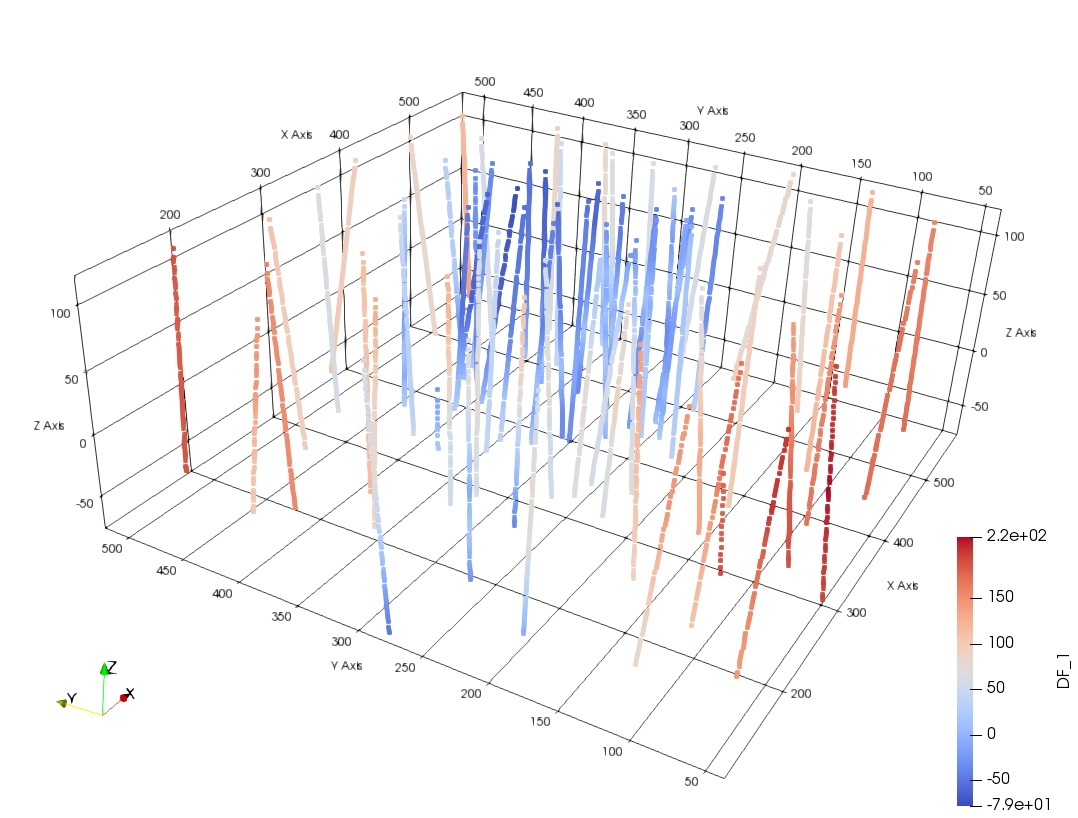
\includegraphics[width=.3\textwidth]{capitulo_2/df1.jpeg}\label{<figure1>}}
     \subfloat[][Categoria 2]{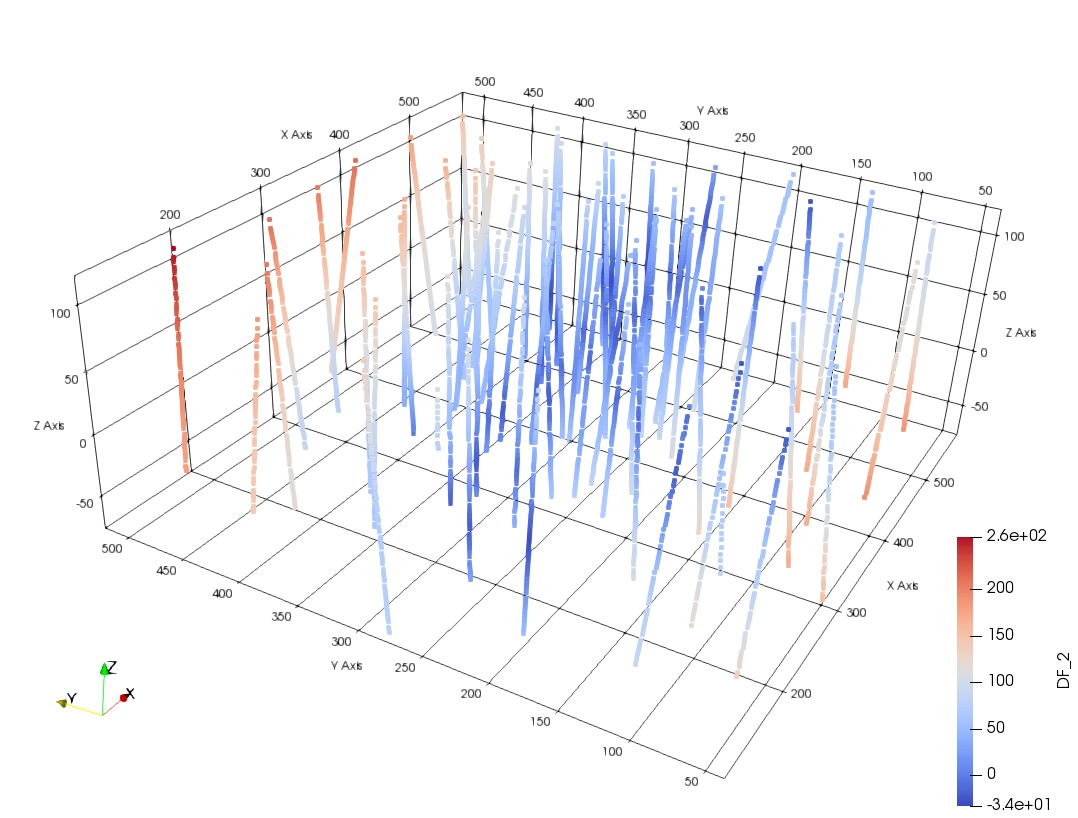
\includegraphics[width=.3\textwidth]{capitulo_2/df2.jpeg}\label{<figure2>}}
     \subfloat[][Categoria 3]{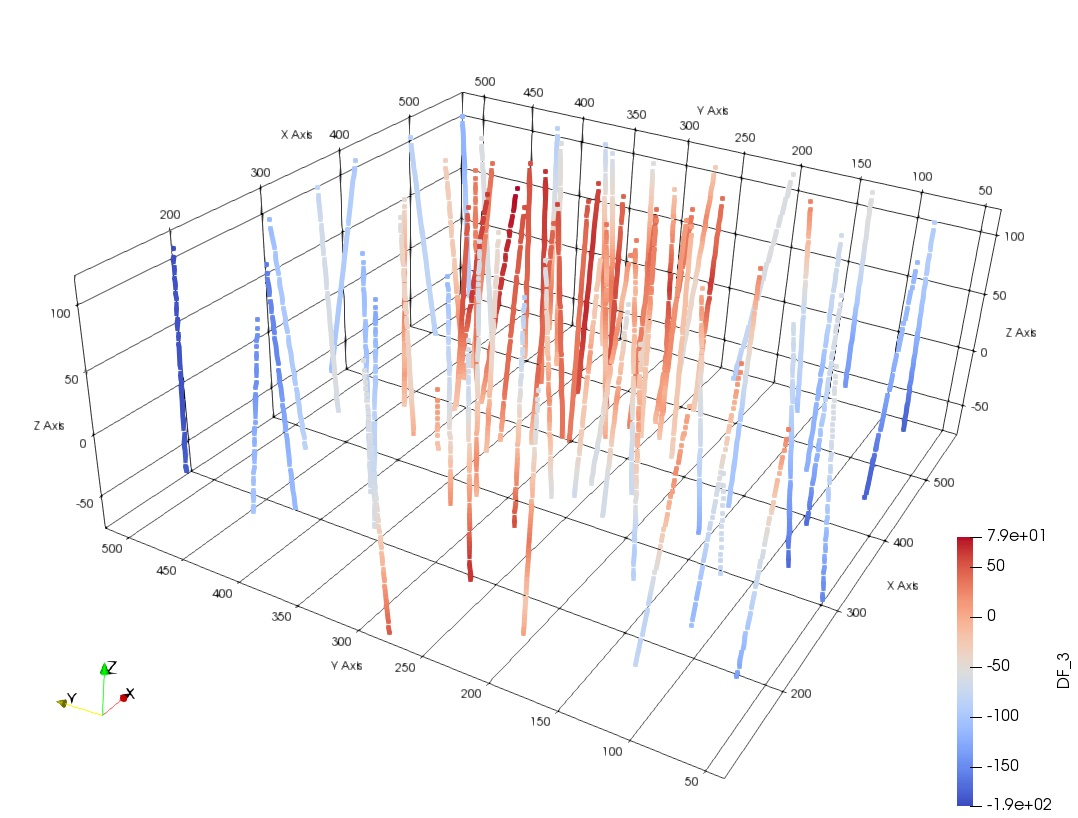
\includegraphics[width=.3\textwidth]{capitulo_2/df3.jpeg}\label{<figure2>}}
\end{figure}

Para corpos geológicos que se estendem muito mais em uma direção em relação às demais, como os corpos tabulares por exemplo, as distâncias calculadas podem ser anisotrópicas. Sendo assim, as coordenadas originais $x$, $y$ e $z$ dos dados devem ser rotacionadas e/ou contraídas/dilatadas, a partir da transformação da \autoref{eq_rot_matrix}. Então, as distâncias euclideanas (\autoref{eq_mult_sg}) são calculadas normalmente para as novas coordenadas $x''$, $y''$, $z''$.

\begin{equation}
\resizebox{.9 \textwidth}{!}{%
$
\begin{bmatrix} x'' \\ y'' \\ z'' \end{bmatrix} = \begin{bmatrix} \frac{1}{a_{max}} & 0 & 0 \\ 0 & \frac{1}{a_{min}} & 0 \\ 0 & 0 & \frac{1}{a_{vert}} \end{bmatrix} \\ \begin{bmatrix}\cos\alpha\cos\phi-\sin\alpha\sin\beta\sin\phi & -\sin\alpha\cos\phi-\cos\alpha\sin\beta\sin\phi & \cos\beta\sin\phi \\ \sin\alpha\cos\beta & \cos\alpha\cos\beta & \sin\beta \\ -\cos\alpha\sin\phi-\sin\alpha\sin\beta\cos\phi & \sin\alpha\sin\phi-\cos\alpha\sin\beta\cos\phi & \cos\beta\cos\phi \end{bmatrix} \begin{bmatrix} x \\ y \\ z \end{bmatrix}
$
}
\label{eq_rot_matrix}
\end{equation}

Onde $a_{max}$, $a_{min}$ e $a_{vert}$ são as dimensões dos eixos máximo, médio e mínimo de anisotropia, e $\alpha$, $\beta$ e $\phi$, os ângulos de azimute, mergulho e \textit{rake}, respectivamente.

\section{Variografia das distâncias calculadas}

No caso das distâncias assinaladas, obter um modelo de covariância a partir dos variogramas experimentais não é trivial. Distâncias assinaladas não são estacionárias, o variograma não se estabiliza em um patamar. Além disso, o caráter extremamente contínuo das distâncias torna a identificação analítica das direções principais um processo embaraçoso.

\citeonline{manchuck_deutsch_Geometric} sugerem alternativas para modelagem do variograma das distâncias:

\begin{itemize}
    \item Treinar o variograma usando validação cruzada;
    \item Tentar modelar interativamente os variogramas experimentais;
    \item Calcular e modelar os variogramas para as propriedades de indicadores e transformá-los em um equivalente gaussiano para as distâncias assinaladas;
    \item inferir um modelo de covariância plausível visualmente a partir das amostras ou de mapas delineados a mão.
\end{itemize}

O alcance do variograma, juntamente com a anisotropia, controlam a extensão e forma dos domínios modelados. Os variogramas experimentais das distâncias assinaladas nunca exibem efeito pepita. Porém, pode ser adicionado arbitrariamente pelo usuário para controlar a interconectividade dos domínios, adicionar ruído ao modelo quando desejável e controlar a extrapolação que pode ser ser excessiva em alguns casos devido a alta continuidade dos modelos Gaussianos.

Os variogramas experimentais das distâncias assinaladas e dos indicadores foram calculados para todas as categorias do banco de dados. A categoria 1 
é uma intrusão vertical. Então foi calculado o variograma omnidirecional no plano horizontal e na direção vertical. A categoria 2 é um intrusão tabular (veio) com direção N351 e mergulho -48. Sendo assim, foi calculado o variograma experimental omnidirecional no plano de atitude e na direção perpendicular ao plano. A categoria 3 é a rocha encaixante, as direções foram as mesmas da categoria 1. A \autoref{par_calc} mostra os parâmetros usados no cálculo dos variogramas experimentais das distâncias assinaladas e dos indicadores.

\begin{table}[H]
\centering
\resizebox{\textwidth}{!}{%
\begin{tabular}{cccccc}
Número de lags & Distância do lag & Tolerância linear & Tolerância do azimute & Tolerância do mergulho & Banda horizontal \\ \hline
50            & 5m               & 2.5m              & 90                   & 22.5                  & 20m              \\ \hline
\end{tabular}%
}
\caption{Parâmetros de cálculo dos variogramas experimentais.} \label{par_calc}
\end{table}

O modelo mais indicado para modelar o variograma das distâncias assinaladas é o modelo Gaussiano. A \autoref{sd_var} mostra os variogramas experimentais e modelos ajustados das distâncias assinaladas para cada uma das categorias do banco de dados. Os modelos foram ajustados de forma automática pelo software PyGeostat \autoref{pygeostat}, com efeito pepita de 0.01 (para evitar instabilidades nas matrizes de krigagem), uma estrutura Gaussiana, patamar estandardizado e com um máximo de 2500 iterações.  

\begin{figure}[H] 
\caption{Variogramas experimentais das distâncias assinaladas e modelos para cada uma das categorias do banco de dados.} \label{sd_var}
     \centering
     \subfloat[][Categoria 1]{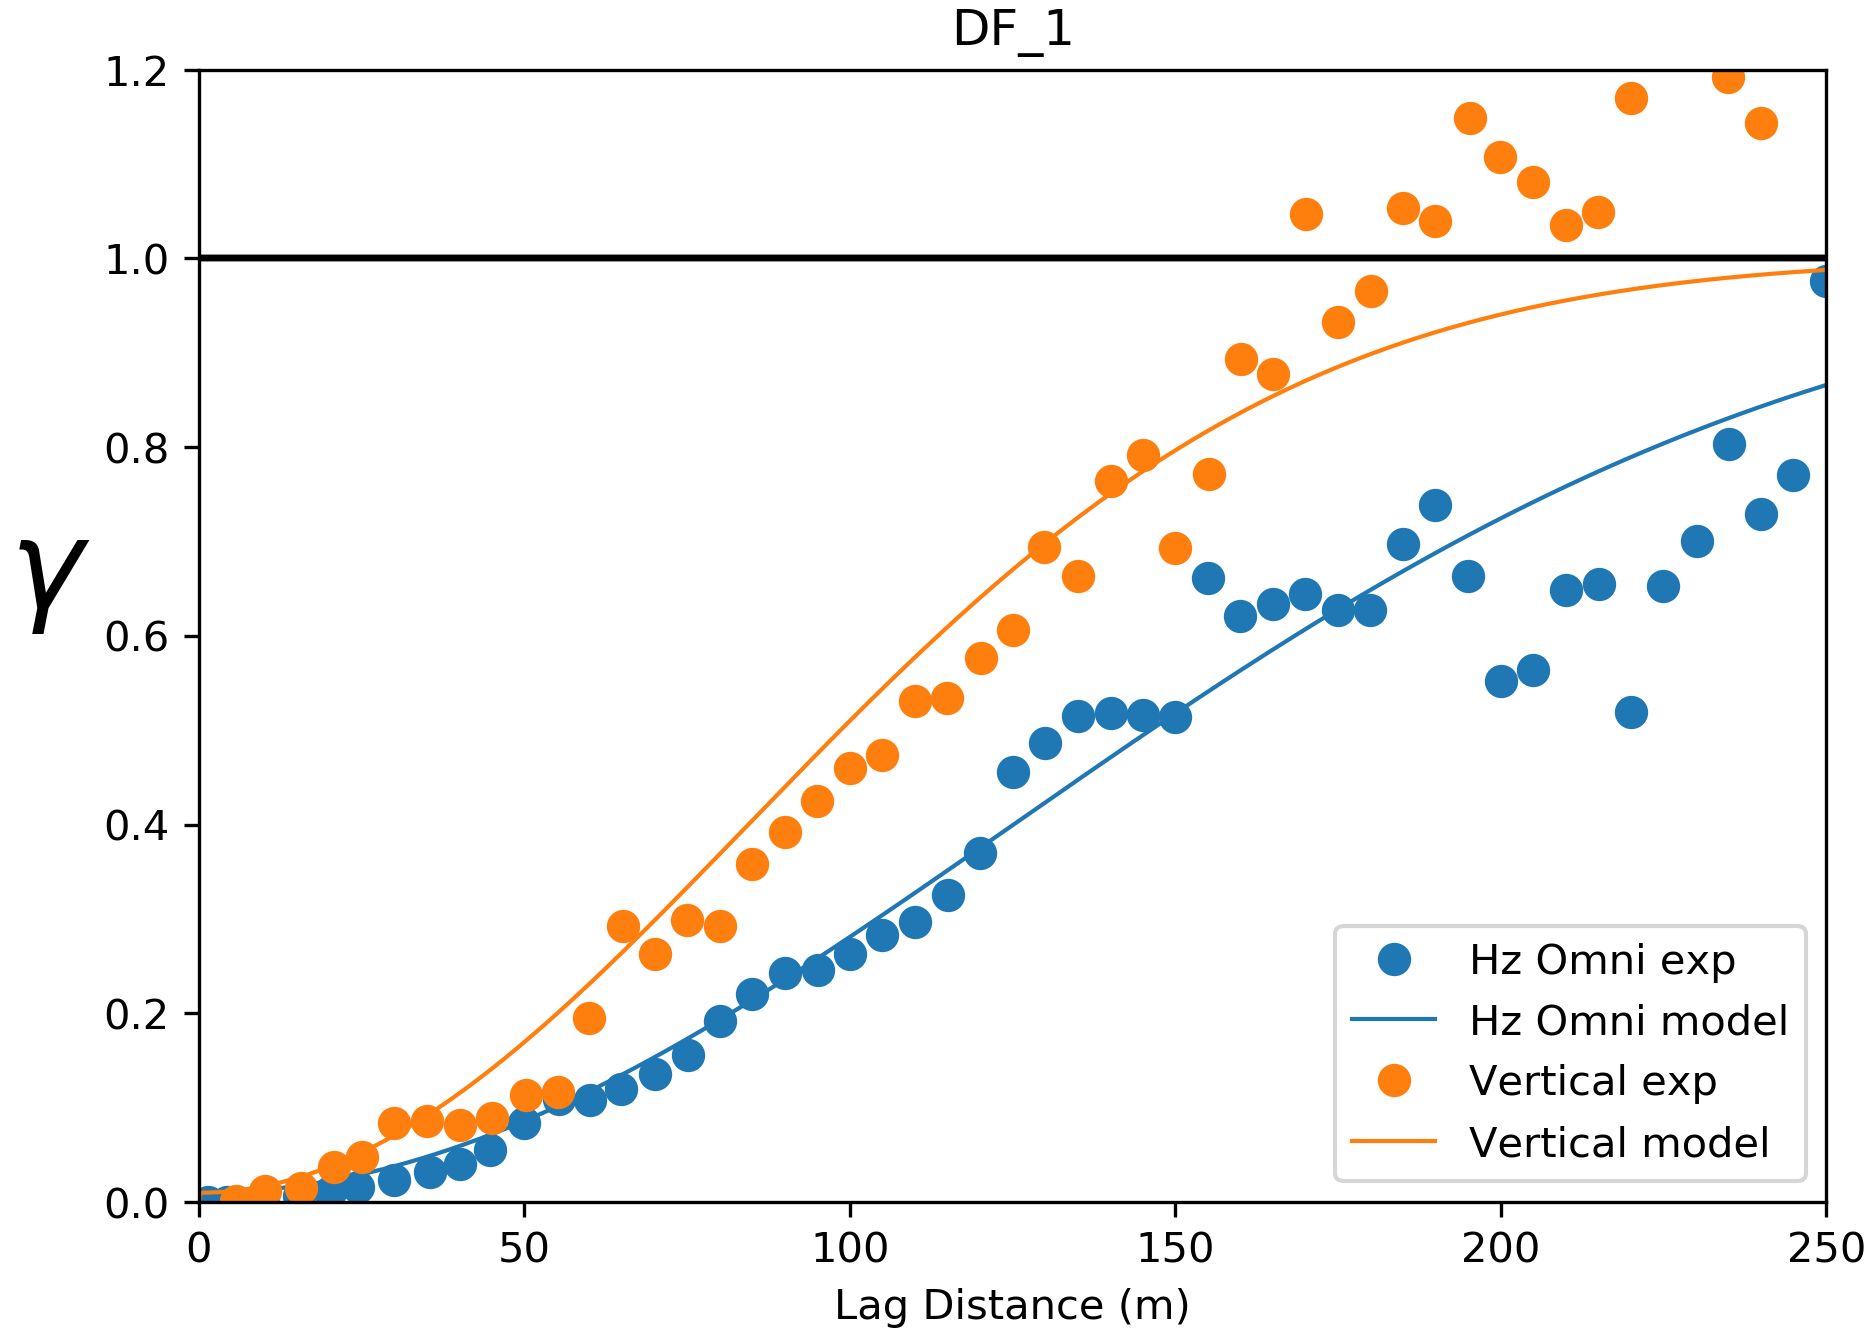
\includegraphics[width=.3\textwidth]{capitulo_2/var_DF_1.png}\label{<figure1>}}
     \subfloat[][Categoria 2]{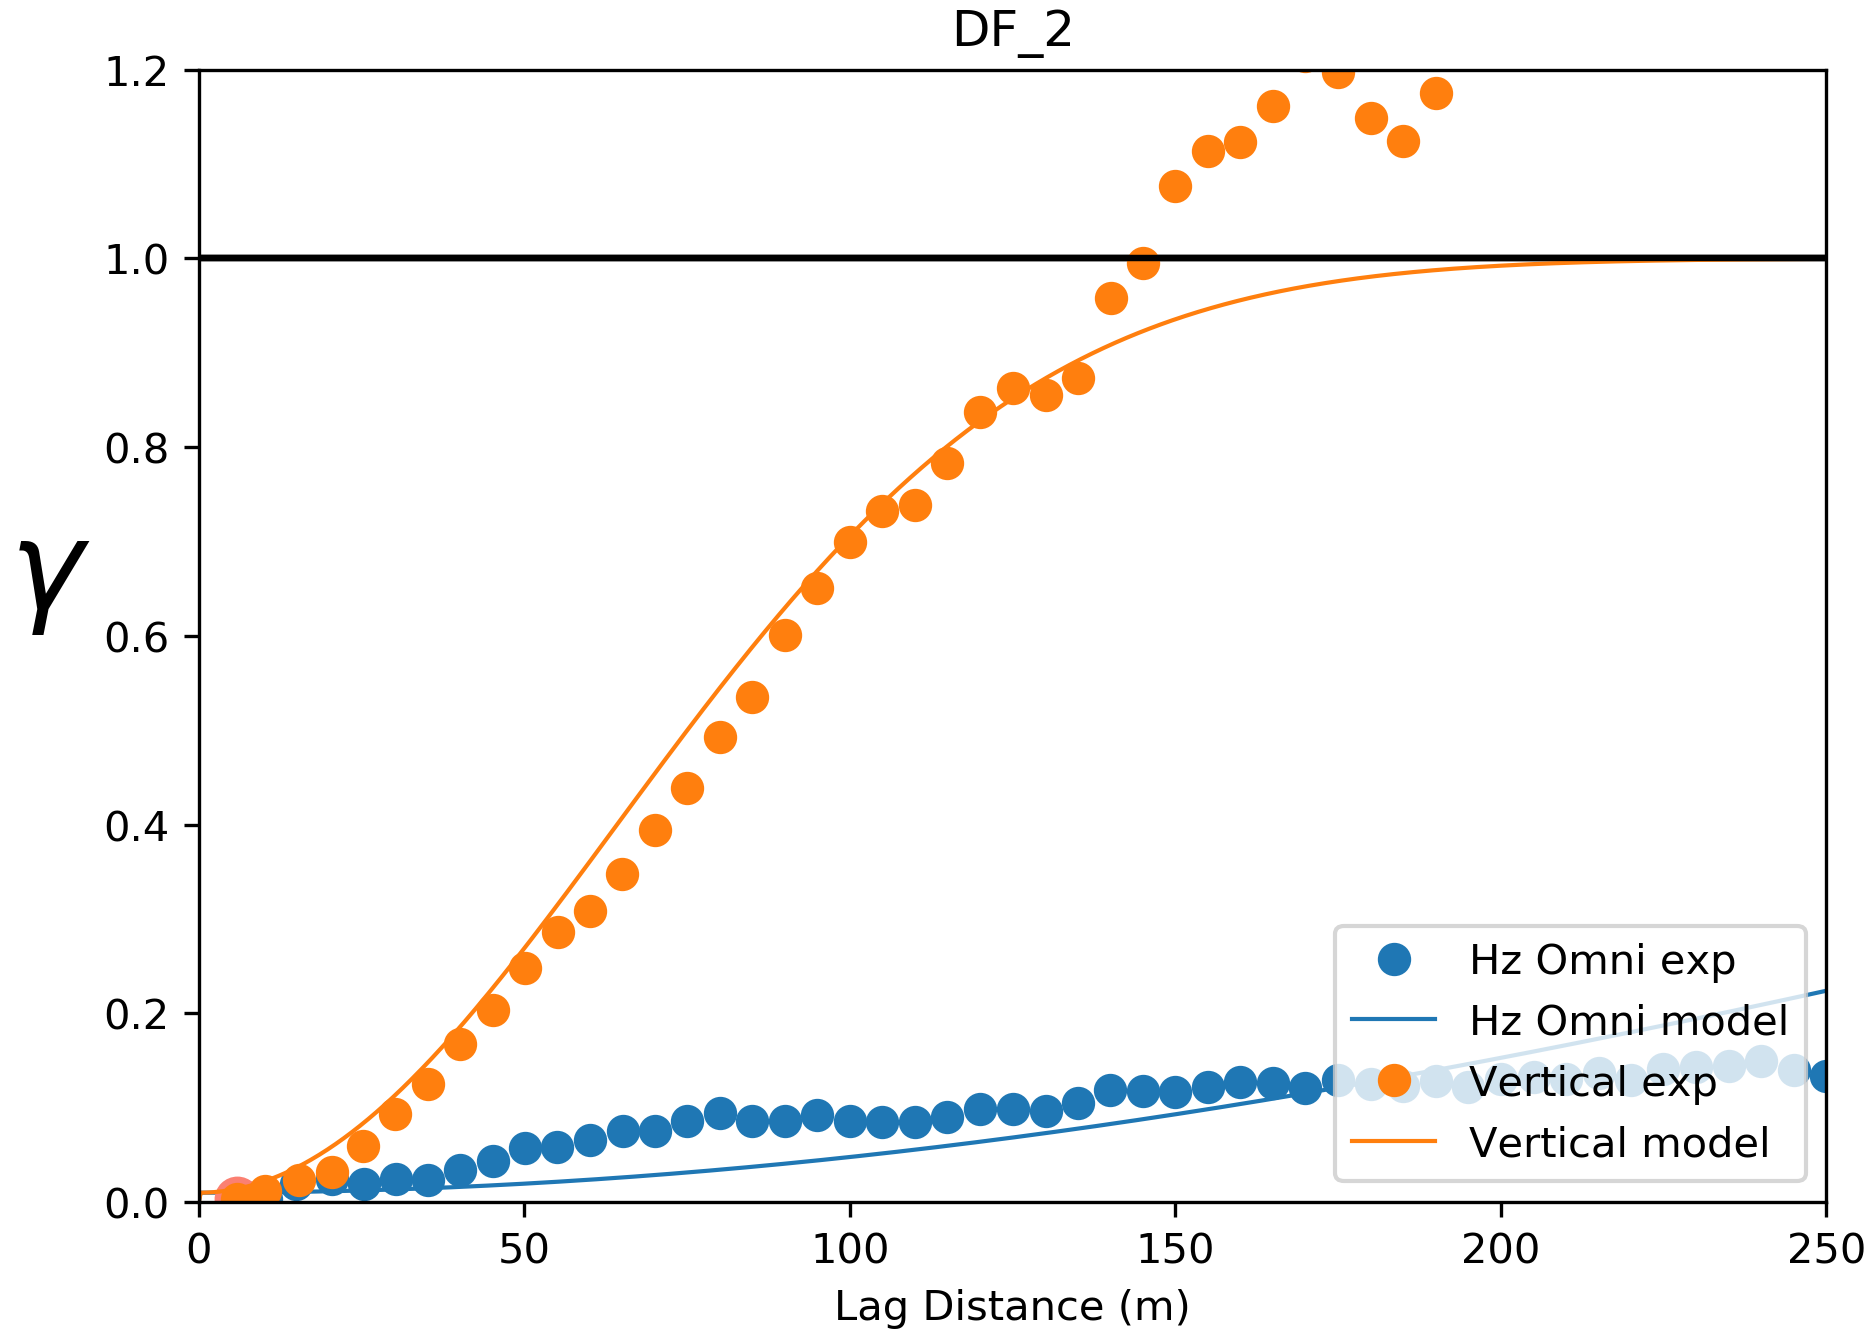
\includegraphics[width=.3\textwidth]{capitulo_2/var_DF_2.png}\label{<figure2>}}
     \subfloat[][Categoria 3]{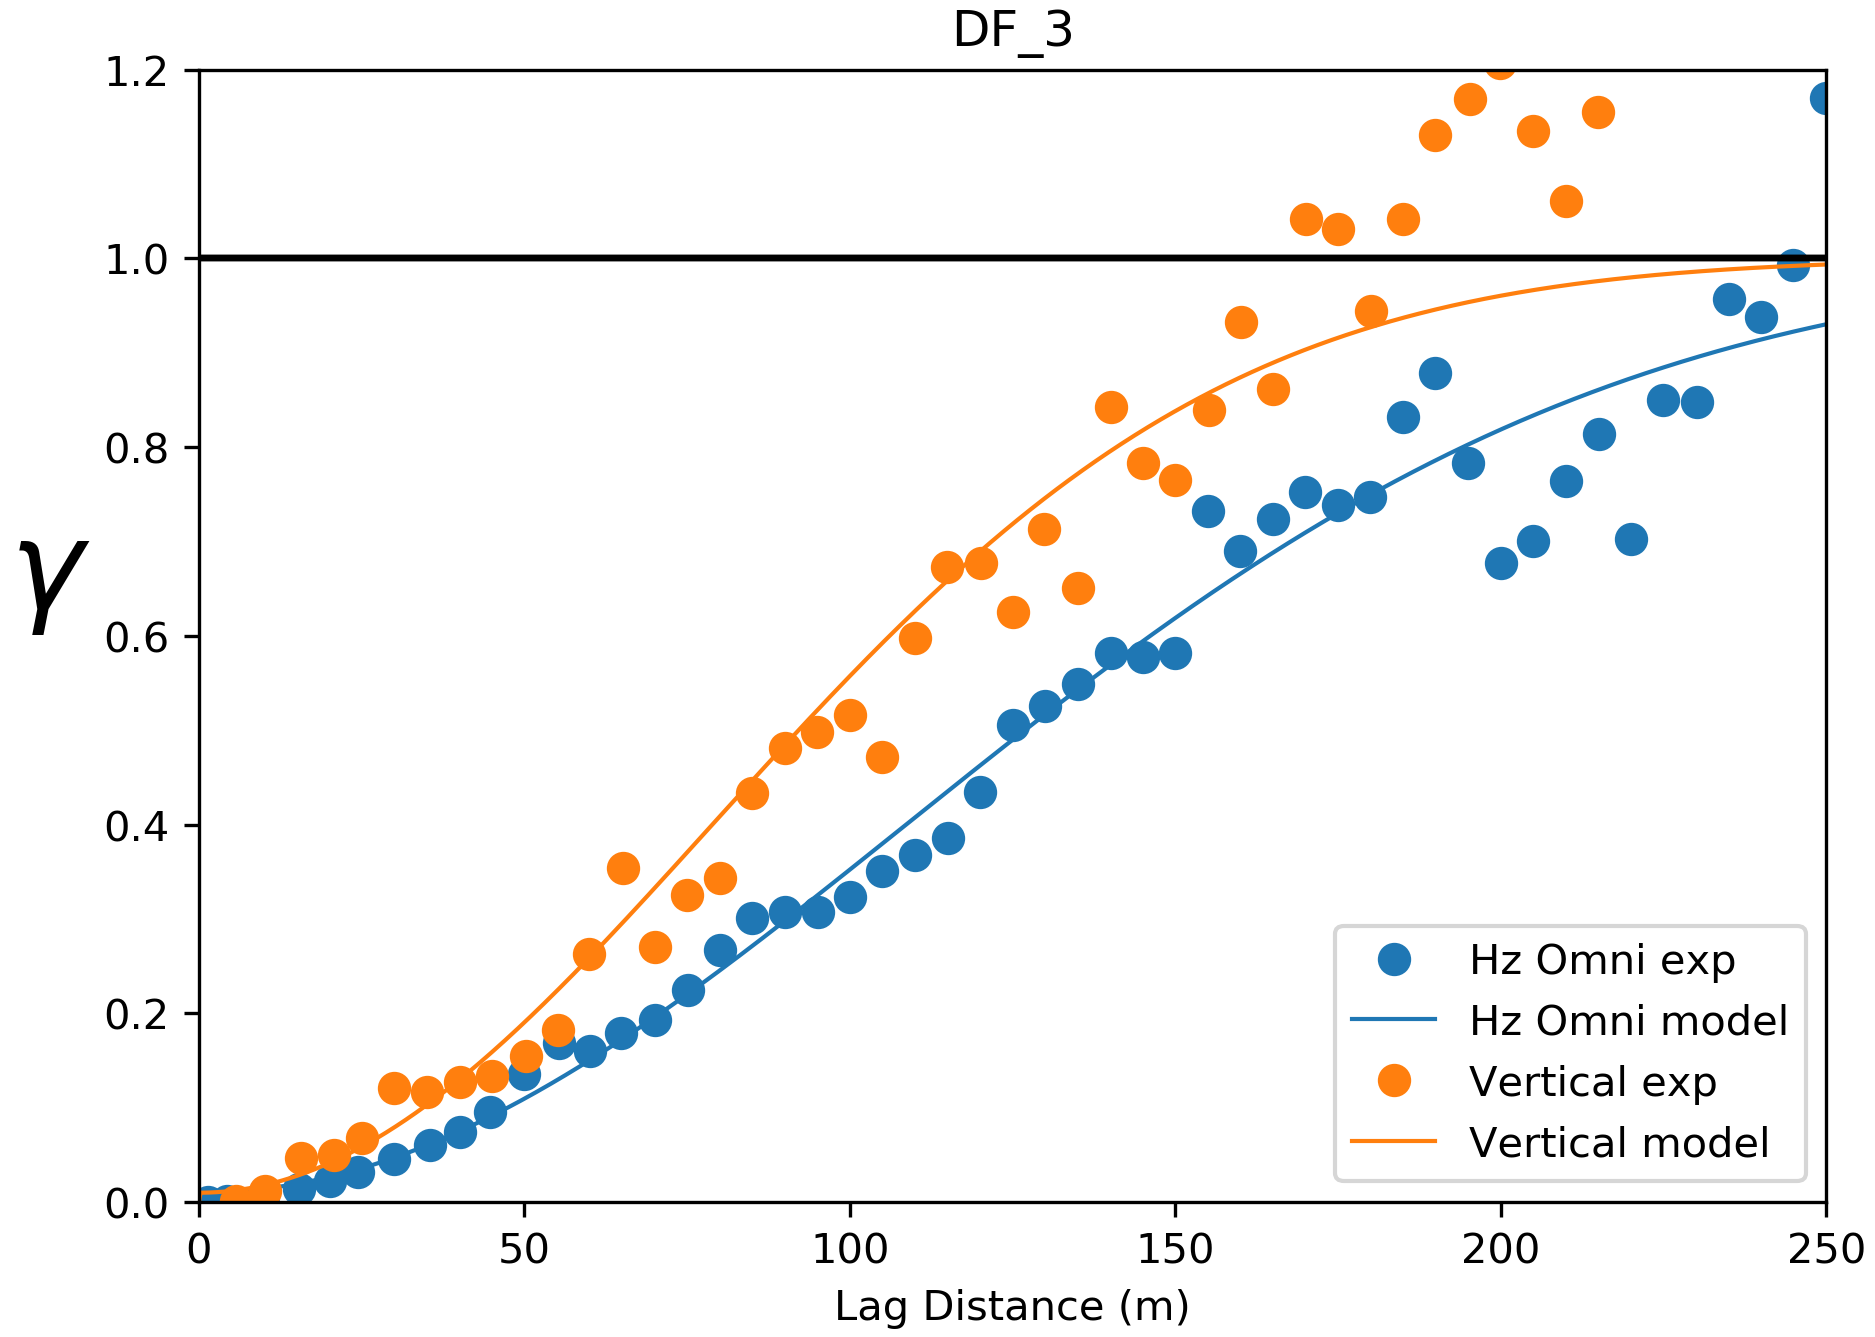
\includegraphics[width=.3\textwidth]{capitulo_2/var_DF_3.png}\label{<figure2>}}
\end{figure}

Os modelos variográficos para cada categoria são expressos pelas \autoref{varsd1}, \autoref{varsd2} e \autoref{varsd3}.

\begin{equation}
\label{varsd1}
\gamma_{SD1}(h)=0.01+0.99gauss\left(\frac{h_{omni}}{306m}, \frac{h_{normal}}{206m}\right)
\end{equation}

\begin{equation}
\label{varsd2}
\gamma_{SD2}(h)=0.01+0.99gauss\left(\frac{h_{omni}}{877m}, \frac{h_{normal}}{157m}\right)
\end{equation}

\begin{equation}
\label{varsd3}
\gamma_{SD3}(h)=0.01+0.99gauss\left(\frac{h_{omni}}{265m}, \frac{h_{normal}}{193m}\right)
\end{equation}

O modelo mais indicado para modelar o variograma dos indicadores é o modelo esférico. A \autoref{ind_var} mostra os variogramas experimentais e modelos ajustados para os indicadores de cada uma das categorias do banco de dados. Os modelos foram ajustados de forma automática pelo software PyGeostat \autoref{pygeostat}, com efeito pepita de 0, uma estrutura esférica, patamar estandardizado e com um máximo de 2500 iterações. 

\begin{figure}[H] 
     \caption{Variogramas experimentais dos indicadores e modelos para cada uma das categorias do banco de dados.} \label{ind_var}
     \centering
     \subfloat[][Categoria 1]{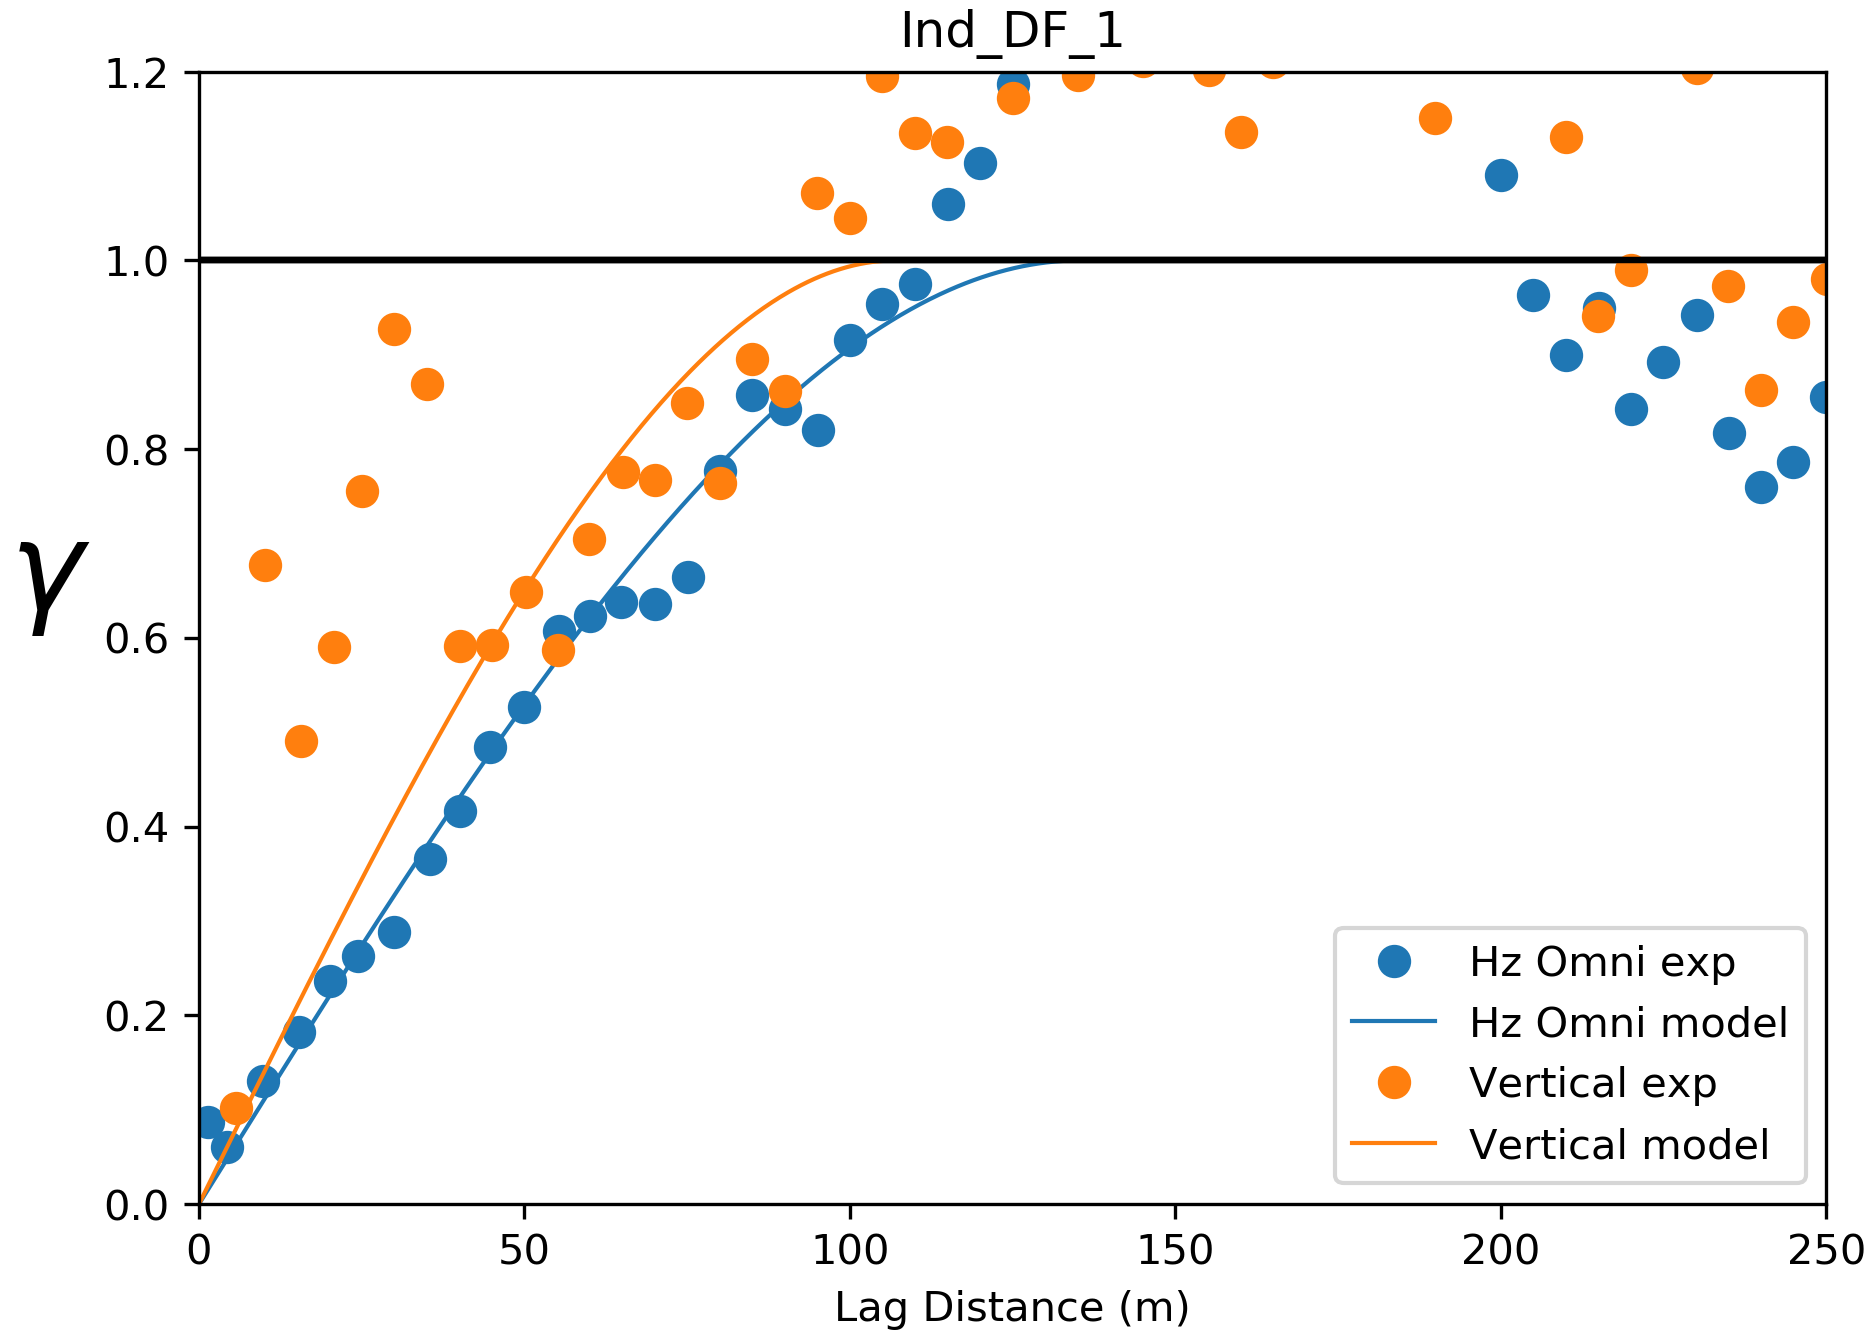
\includegraphics[width=.3\textwidth]{capitulo_2/var_Ind_DF_1.png}\label{<figure1>}}
     \subfloat[][Categoria 2]{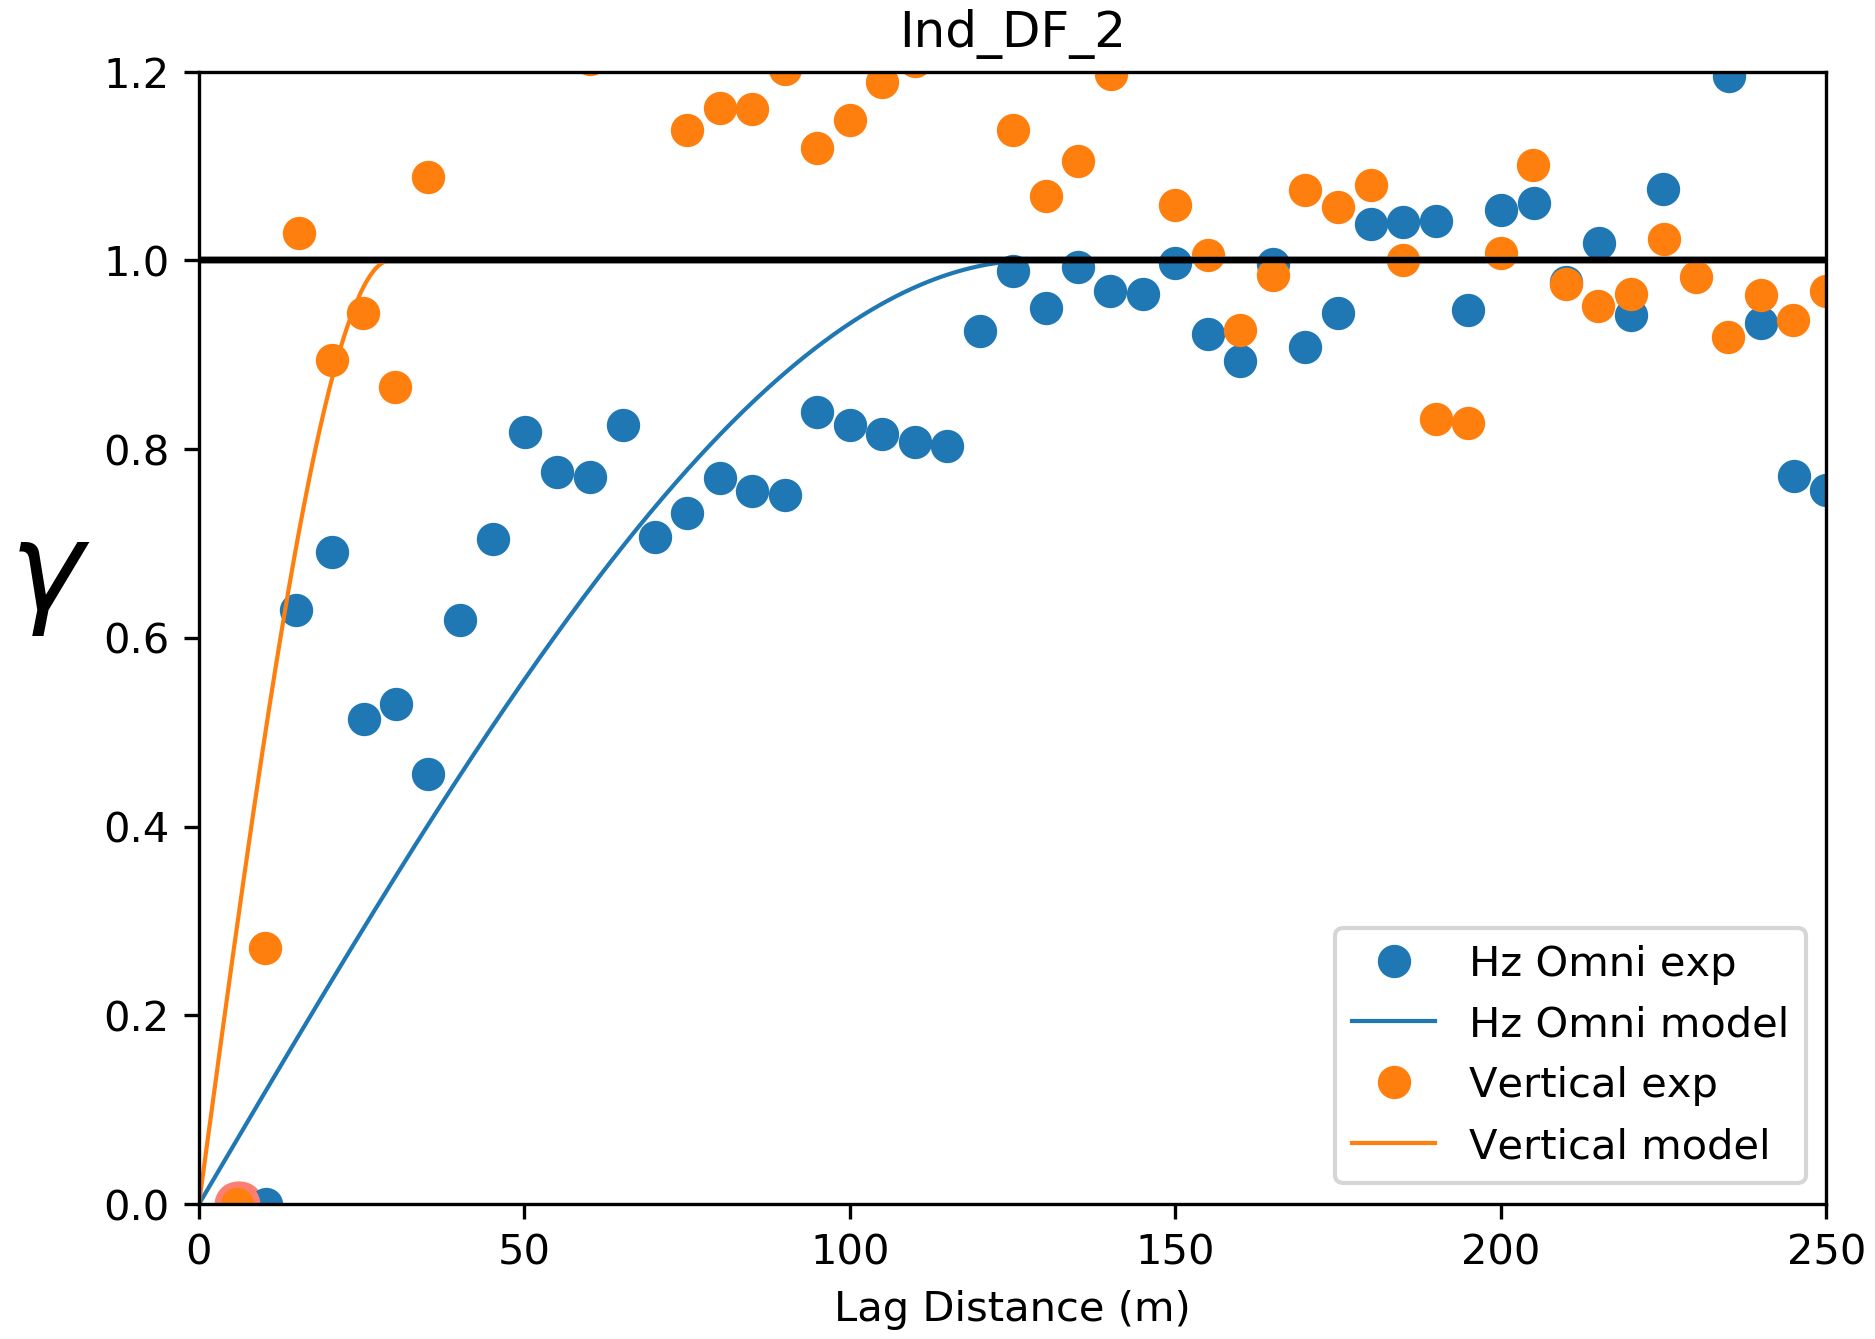
\includegraphics[width=.3\textwidth]{capitulo_2/var_Ind_DF_2.png}\label{<figure2>}}
     \subfloat[][Categoria 3]{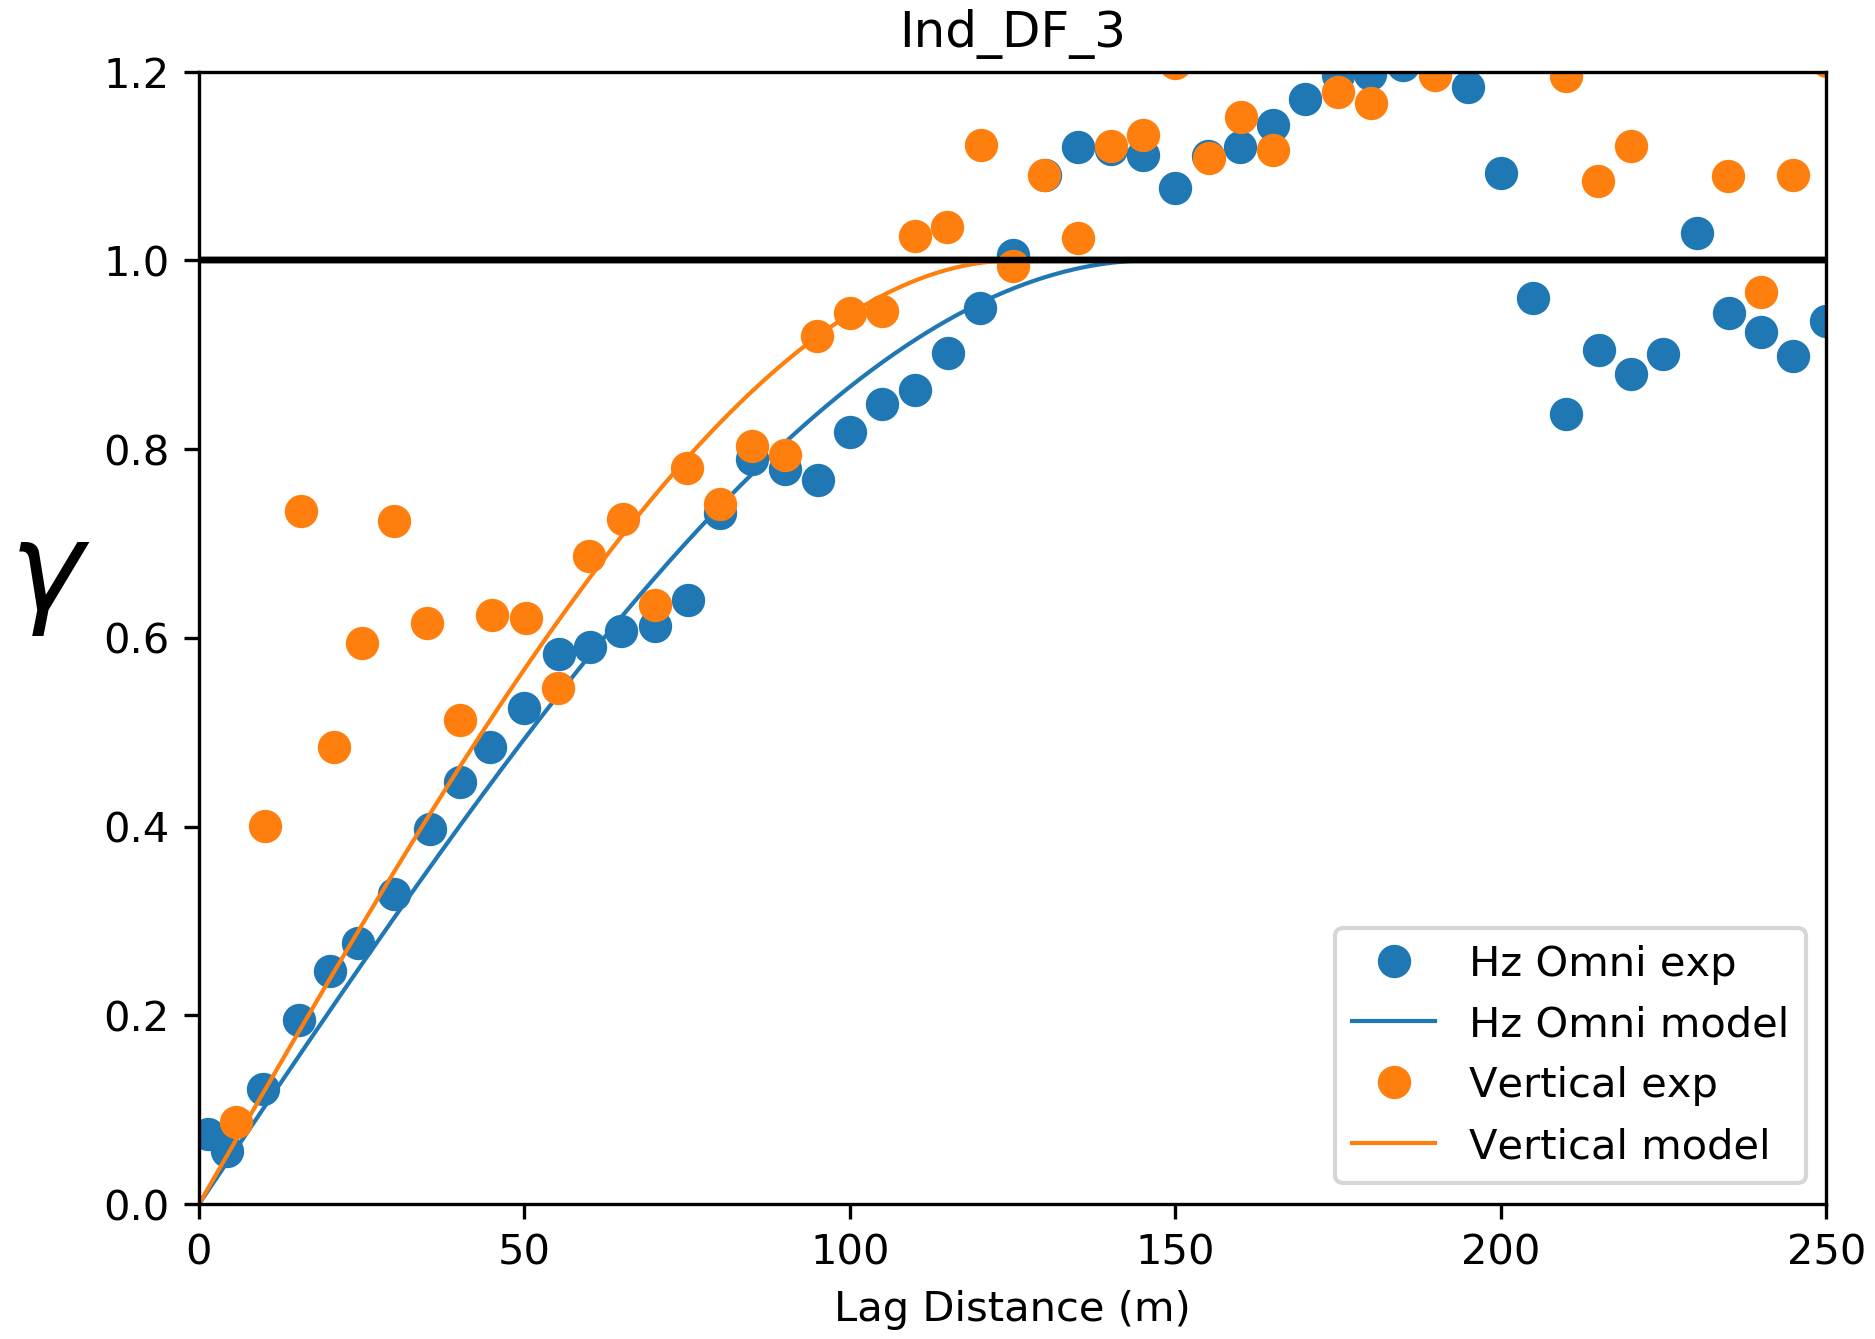
\includegraphics[width=.3\textwidth]{capitulo_2/var_Ind_DF_3.png}\label{<figure2>}}
\end{figure}

Os modelos variográficos para cada categoria são expressos pelas \autoref{varind1}, \autoref{varind2} e \autoref{varind3}.

\begin{equation}
\label{varind1}
\gamma_{IND1}(h)=1.0sph\left(\frac{h_{omni}}{135m}, \frac{h_{normal}}{106m}\right)
\end{equation}

\begin{equation}
\label{varind2}
\gamma_{IND2}(h)=1.0sph\left(\frac{h_{omni}}{128m}, \frac{h_{normal}}{29m}\right)
\end{equation}

\begin{equation}
\label{varind3}
\gamma_{IND3}(h)=1.0sph\left(\frac{h_{omni}}{146m}, \frac{h_{normal}}{125m}\right)
\end{equation}

Em teoria, o ajuste dos variogramas dos indicadores é mais fácil se comparado ao variograma das distâncias assinaladas, além de atingirem um patamar, a menor continuidade espacial em relação às distâncias torna a identificação analítica das direções principais um processo mais simples. No entanto, muitas vezes, na prática se observa o contrário.

Uma outra alternativa ao cálculo e modelagem de variogramas é o uso de tabelas de covariância proposto por \citeonline{kloechner_cov_table}, onde propõem a substituição da modelagem tradicional dos variogramas por tabelas de covariância, tornando o processo de modelagem geológica completamente automático e livre da subjetividade do geomodelador. A \autoref{cov_table} mostra o fluxograma da metodologia proposta.

\begin{figure}[H]
	\caption{\label{cov_table}Fluxograma da modelagem geológica implícita usando tabelas de covariância.}
	\begin{center}
		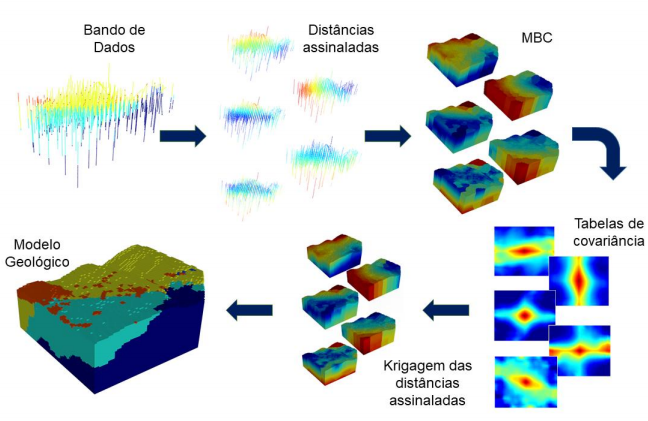
\includegraphics[width=0.7\textwidth]{capitulo_2/cov_table.png}
	\end{center}
	\legend{\citeonline{kloechner_cov_table}}
\end{figure}

O trabalho propõe uma técnica para obter uma tabela de covariância, a partir de um modelo base, que reproduz a continuidade espacial de um dado atributo usando o teorema de convolução via transformada rápida de Fourier. Embora a metodologia tenha apresentado resultados satisfatórios, a construção automática das tabelas de covariância ainda apresenta alguns problemas operacionais que tornam sua aplicação inviável para todos os tipo de depósito.

\section{Interpolação das distâncias calculadas}

Uma vez que as distâncias tenham sido calculadas a partir da localização das amostras, o próximo passo é interpolar o novo banco de dados para o grid definido para a modelagem geológica. Embora métodos implícitos não demandem um grid - são métodos conhecidos como \textit{gridless} - o objetivo final é preencher o grid de estimativas com as categorias correspondentes ou visualizar o modelo através de iso superfícies. Técnicas de extração de iso superfícies exigem a função volumétrica definida exaustivamente em um grid retilíneo \cite{martin2017implicitmodeling}.

\subsection{Resolução do grid}

Para um número constante de amostras, o tempo necessário para interpolação da função volume para todos os nós do grid aumenta linearmente com o número de nós. Os parâmetros do grid de estimativas, muitas vezes, são determinado por requisitos de engenharia do projeto. Todavia, o grid para definição do modelo geológico pode ser diferente do grid definido para os modelos numéricos de teores. A consideração mais importante é a capacidade de reproduzir a menor estrutura geológica de interesse.

Considere os modelos implícitos da \autoref{grid_res} gerados em grids de diferentes resoluções.

\begin{figure}[H]
	\caption{\label{grid_res}Efeito da resolução do grid na reprodução de estruturas geológicas.}
	\begin{center}
		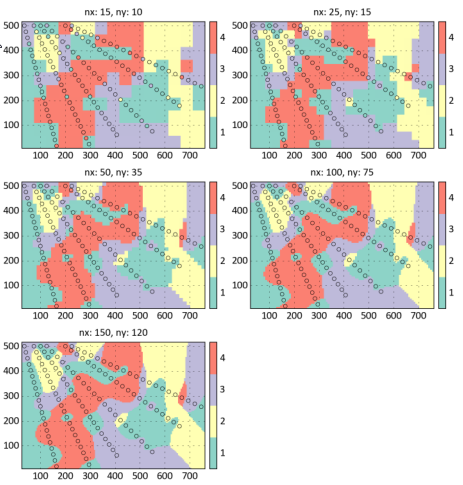
\includegraphics[width=0.6\textwidth]{capitulo_2/grid_res.png}
	\end{center}
	\legend{Fonte: \citeonline{martin2017implicitmodeling}}
\end{figure}

A resolução adequada para esse modelo é entre (nx, ny) = (50, 35) e (nx, ny) = (100, 75). Para os dois primeiros /textit{grids}, há classificação errônea dos nós colocados com amostras, além de (nx, ny) = (100, 75) há pouco benefício na reprodução das estruturas levando em consideração o aumento do tempo de interpolação.

É preciso encontrar um balanço entre resolução e tempo de interpolação. A resolução do grid pode ser aumentada a medida que o projeto avança e mais informação é adquirida \cite{martin2017implicitmodeling}.

Para o estudo de caso, foram gerados dois grids com resoluções diferentes, seus parâmetros são mostrados na \autoref{grid_def}.

\begin{table}[H]
\centering
\begin{tabular}{lrr}
 & \multicolumn{1}{l}{Grosso} & \multicolumn{1}{l}{Fino} \\ \hline
nx & 49 & 97 \\
ny & 49 & 98 \\
nz & 51 & 102 \\
sx & 10m & 5m \\
sy & 10m & 5m \\
sz & 4m & 2m \\
num & 122451 & 969612 \\ \hline
\end{tabular}
\caption{Parâmetros dos grids de definição dos modelos geológicos implícitos.} \label{grid_def}
\end{table}

A \autoref{dif_res} mostra seções em XZ de dois modelos geológicos implícitos gerados em grids com resoluções diferentes para o banco de dados do estudo de caso. No \textit{grid} fino (\autoref{a}), as formas reproduzidas são suaves, apresentam realismo geológico, e o número de classificações errôneas é menor.

\begin{figure}[H]
\caption{Modelos geológicos em diferentes resoluções} 
\label{dif_res}
\begin{center}
\subfloat[][Modelo geológico implícto no grid grosso]{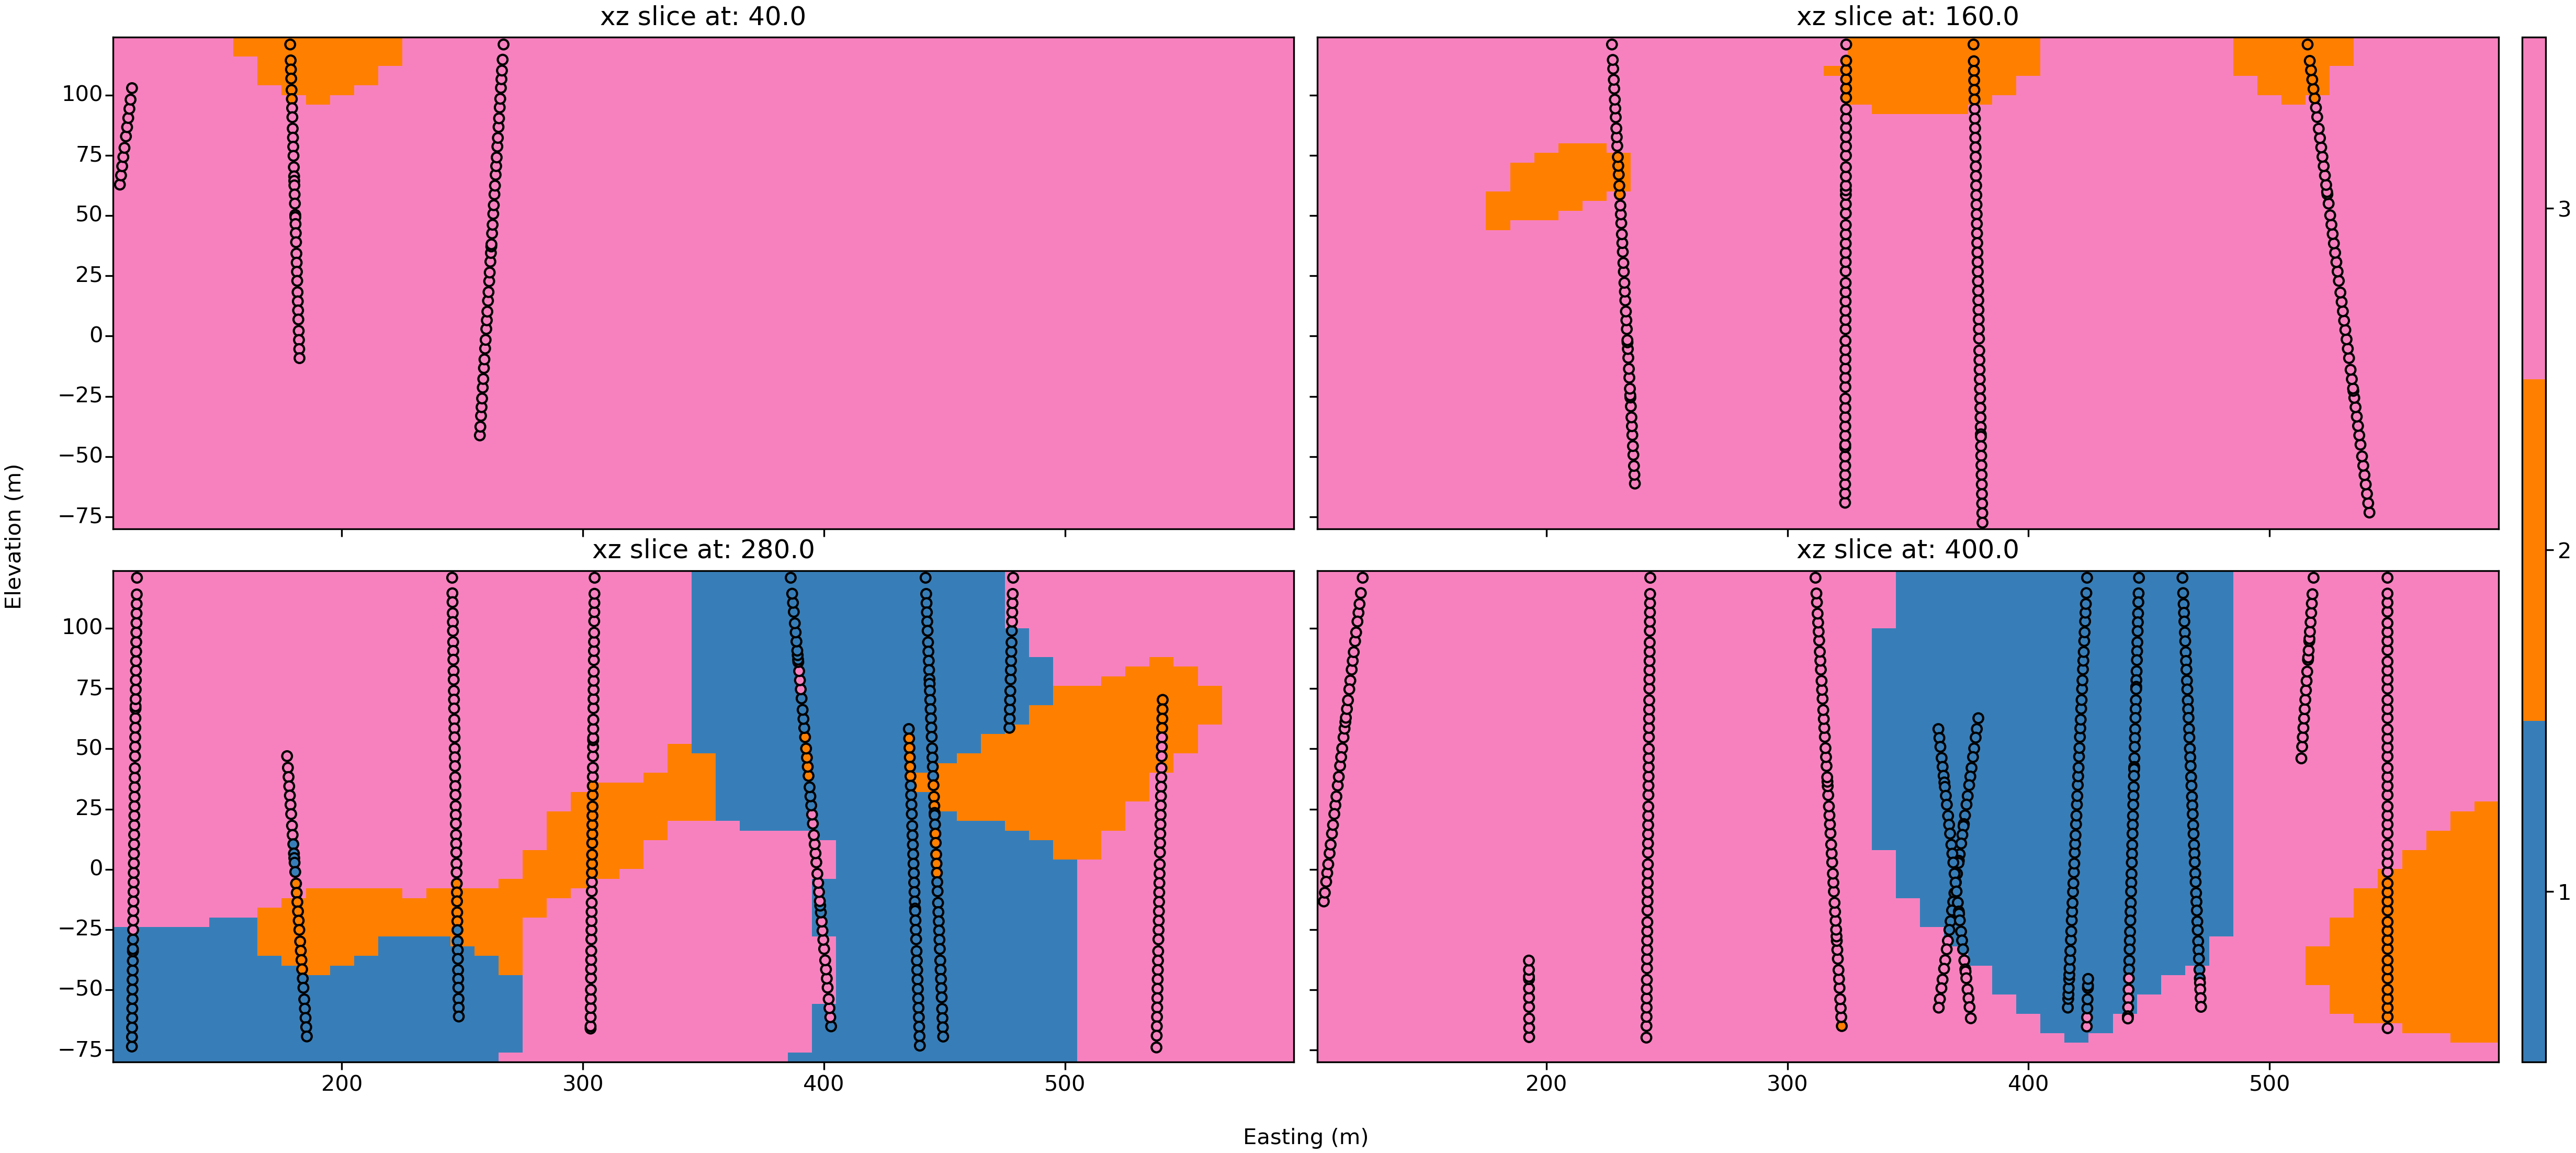
\includegraphics[width=0.8\textwidth]{capitulo_2/coarserxz.png}\label{a}}\\
\end{center}
\begin{center}
\subfloat[][Modelo geológico implícto no grid fino]{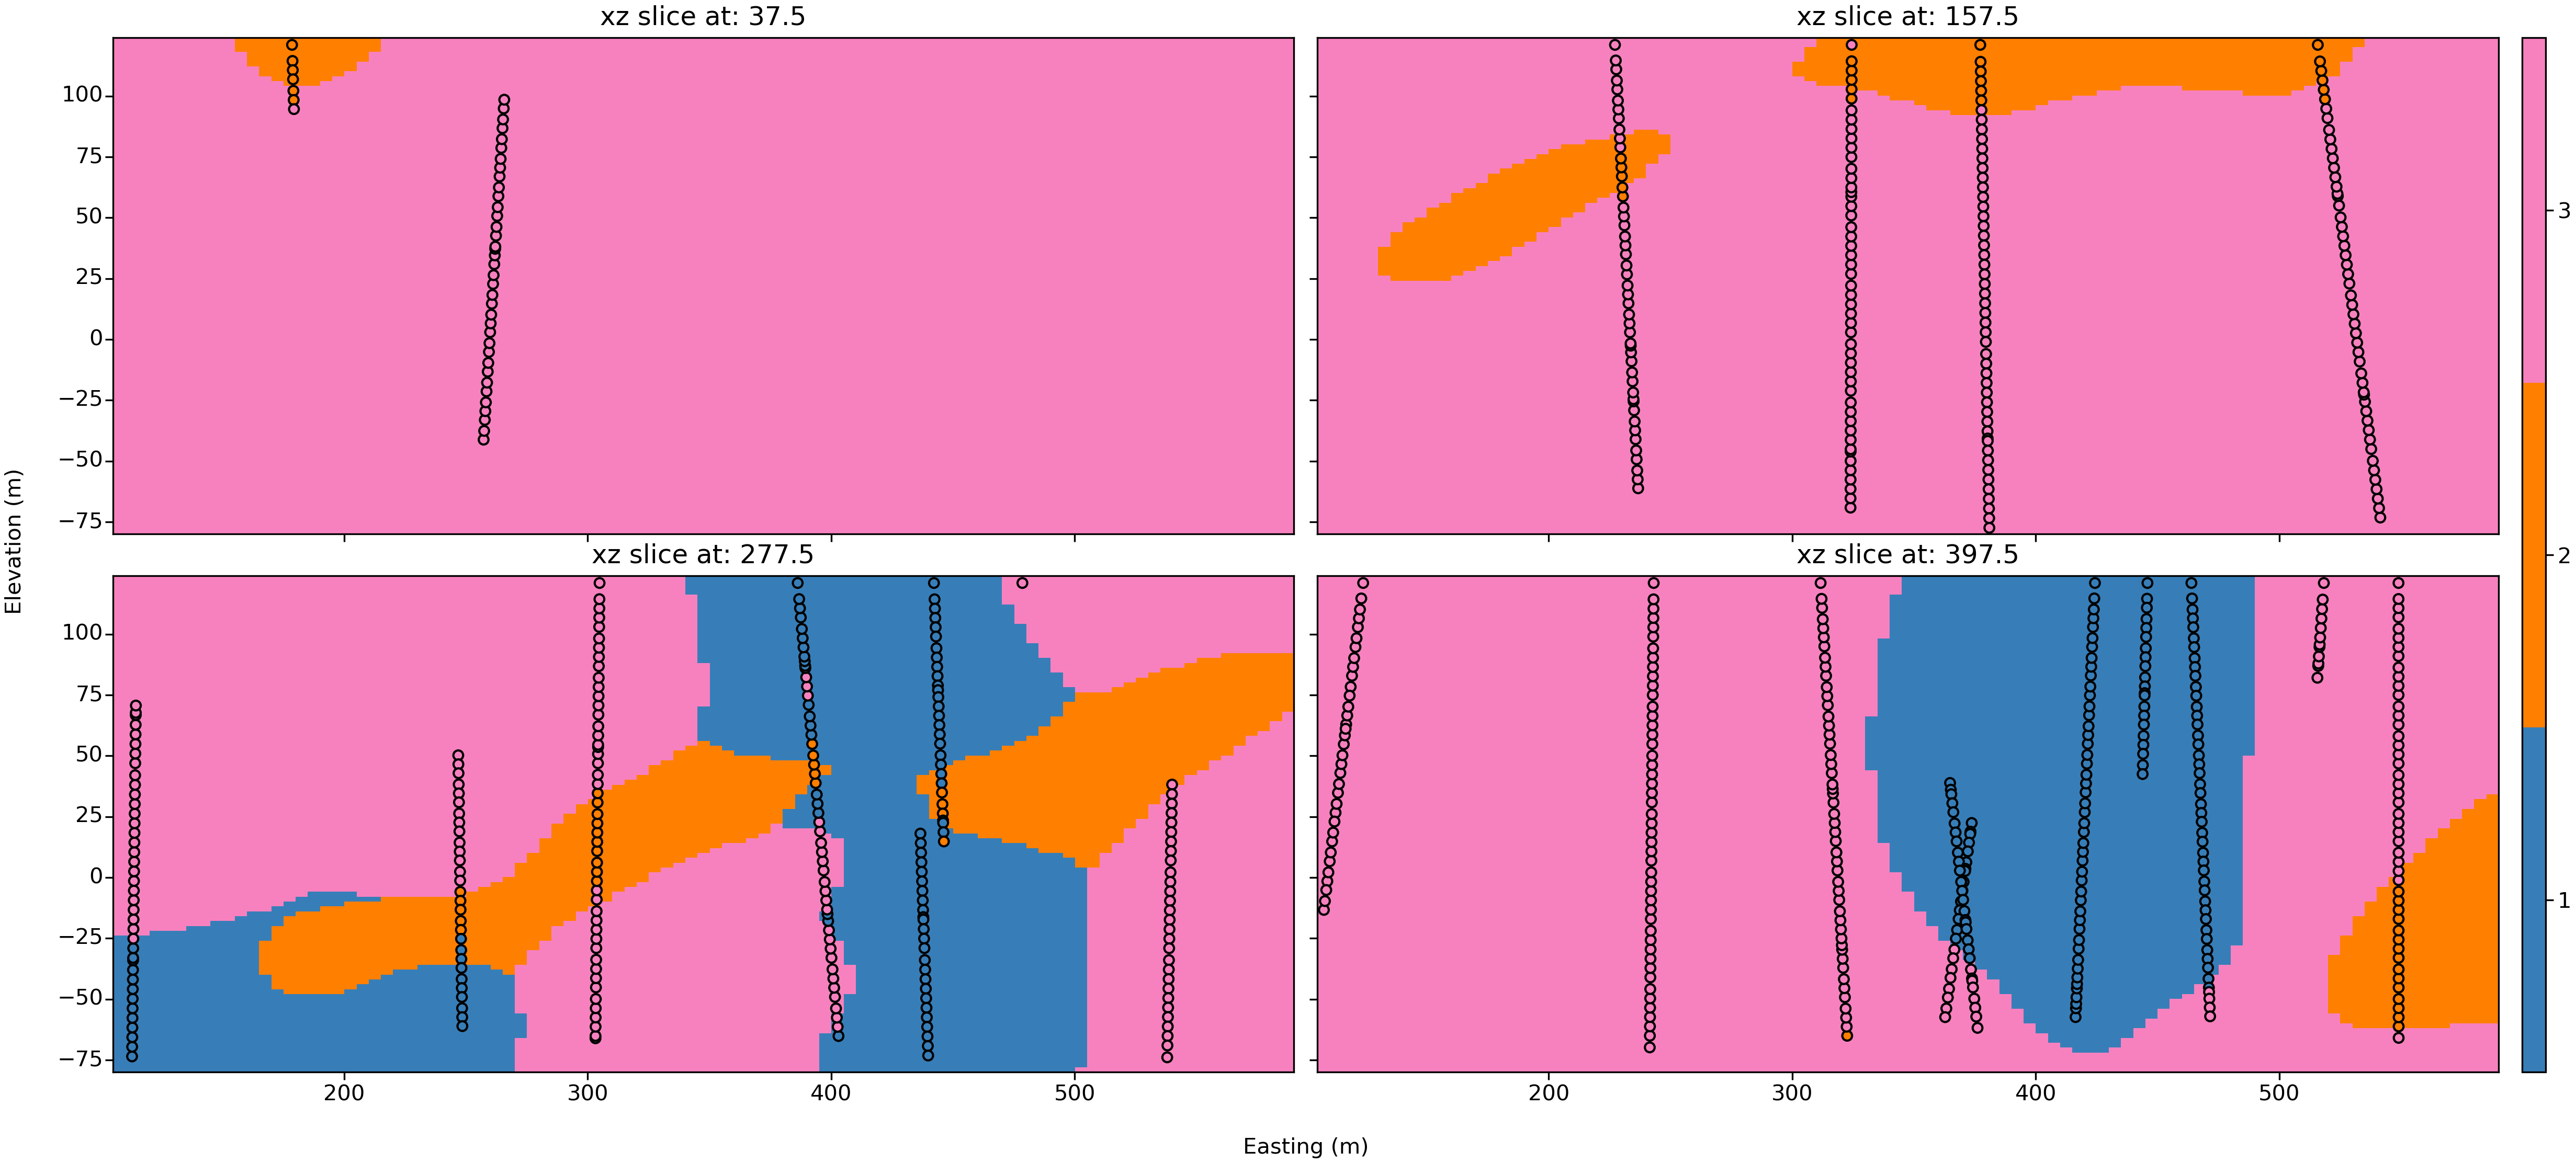
\includegraphics[width=0.8\textwidth]{capitulo_2/finerxz.png}\label{b}}
\end{center}
\end{figure}

\subsection{Métodos de interpolação}\label{met_int}

Qualquer método de interpolação pode ser utilizado para as distâncias assinaladas, mesmo os métodos do inverso da distância produzem resultados realistas. A krigagem e as funções de bases radiais permitem incorporar informação adicional através dos modelos de covariância parametrizados a partir das amostras e minimizam a variância do erro. A literatura recomenda uso de métodos globais, que usam todas as amostras para cada estimativa, para evitar o surgimento de artefatos nos modelos.

\citeonline{hosseini_deutsch_iqd} utilizaram inverso da distância, \citeonline{silvaenhancedgeomodeling} utilizou krigagem ordinária global, \citeonline{rolo_dissertacao} utilizou krigagem ordinária, \citeonline{silva_dual} aplicaram \textit{dual kriging}, \citeonline{boisvert_geomodeling} gerou modelos implícitos através de distâncias assinaladas com anisotropia variável local (\textit{Locally varying anisotropy kriging - LVA}) e \citeonline{cowan2002rapid} propôs a utilização de interpoladores baseados em funções de bases radiais (\textit{radial basis functions - RBF}). \citeonline{manchuck_MLS} ainda propuseram a utilização de mínimos quadrados móveis para incorporar interpretação manual e avaliar incerteza. A escolha do interpolador deve ser baseada em suas propriedades, na informação exigida para parametrizá-lo (o variograma, por exemplo) e nas sua capacidade de se ajustar a formas geológicas.

Além das características de cada interpolador, para as funções distância assinaladas existe um problema adicional relacionado à estacionariedade, de primeira e segunda ordem. Existe uma forte tendência (\textit{trend}) na variável disttância que restringe os estimadores baseados em krigagem à krigagem ordinária para que a estacionariedade seja mantida. Além disso, formas geológicas são curvilíneas e não são bem descritas por funções de covariância lineares. Por esses motivos, muitos autores preferem as funções de bases radiais já que ela não se baseia em estacionariedade de primeira ordem e honra localmente formas geológicas sem a necessidade de parametrização especial \cite{martin2017implicitmodeling}.

Independente do método de interpolação, os modelos gerados devem ser livres de artefatos para que os artefatos do modelo implícito não sejam transferidos para os modelos geológicos. Funções de bases radiais e krigagem global garantem modelos livres de artefato por utilizarem todas as amostras em cada estimativa, já para os métodos baseados em inverso da distância e krigagem (não global) os parâmetros de busca são uma escolha crítica \cite{martin2017implicitmodeling}. No entanto, métodos globais possuem limitações em bancos de dados volumosos por dependerem de muito processamento e memória RAM.

A \autoref{interpo} mostra três modelos implícitos, para a categoria 1, interpolados por krigagem ordinária usando 40 amostras, krigagem ordinária usando 100 amostras e funções de bases radiais, que é um método global. A krigagem ordinária global gerou modelos implícitos extremantes contínuos, mais do que o desejado, implicando em modelos geológicos não realistas. 

\begin{figure}[H] 
    \caption{Interpolação das distâncias calculadas por diferentes métodos.} \label{interpo}
     \centering
     \subfloat[][OK com 40 amostras]{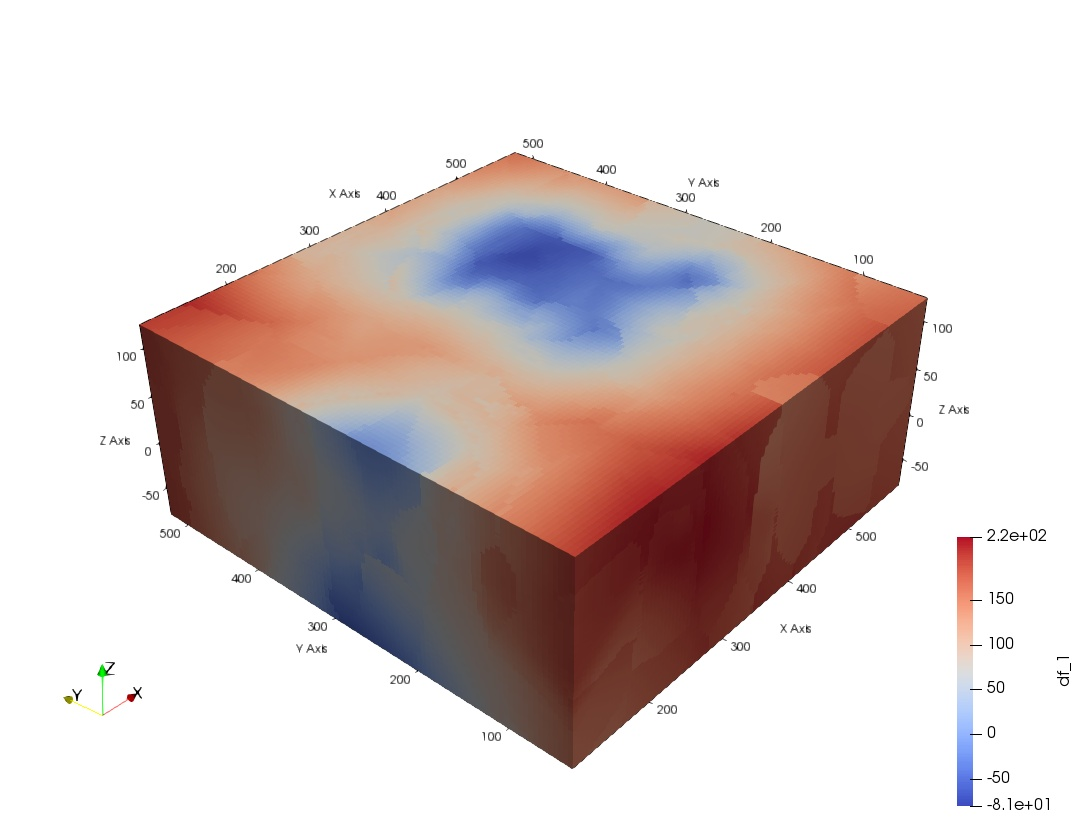
\includegraphics[width=.3\textwidth]{capitulo_2/kt3d40.jpeg}\label{<figure1>}}\\
     \subfloat[][OK com 100 amostras]{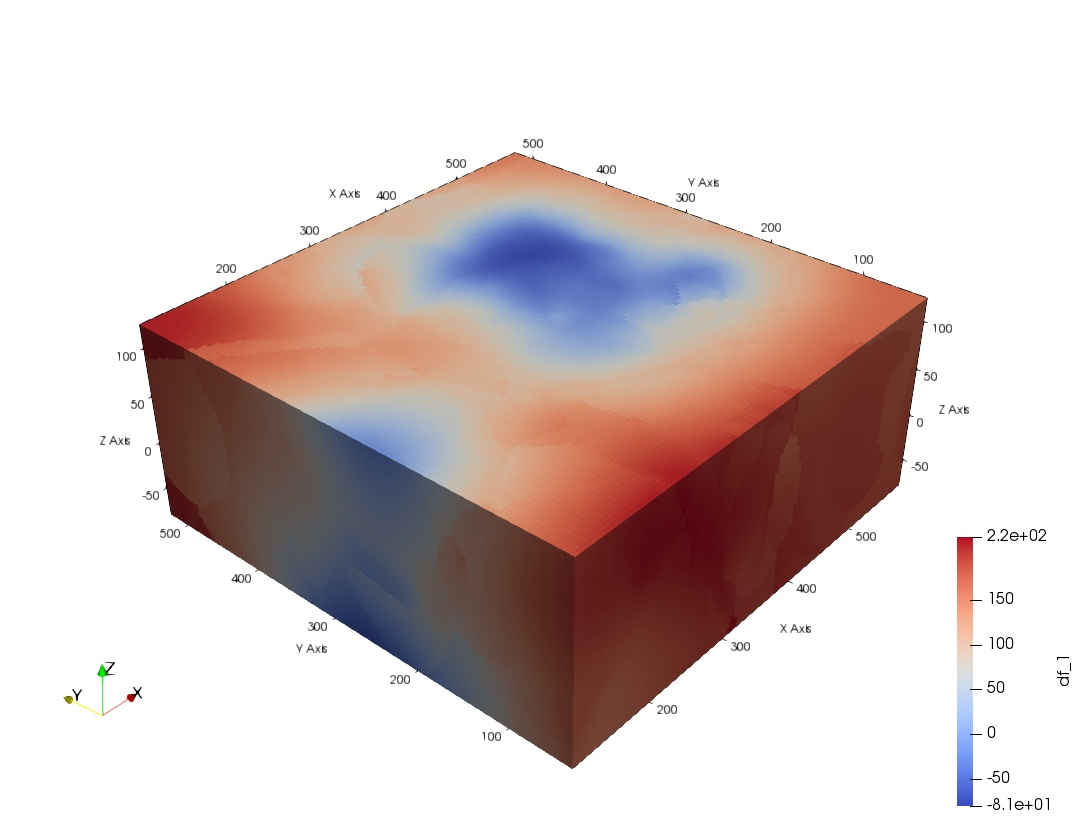
\includegraphics[width=.3\textwidth]{capitulo_2/kt3d100.jpeg}\label{<figure2>}}\\
     \subfloat[][RBF global]{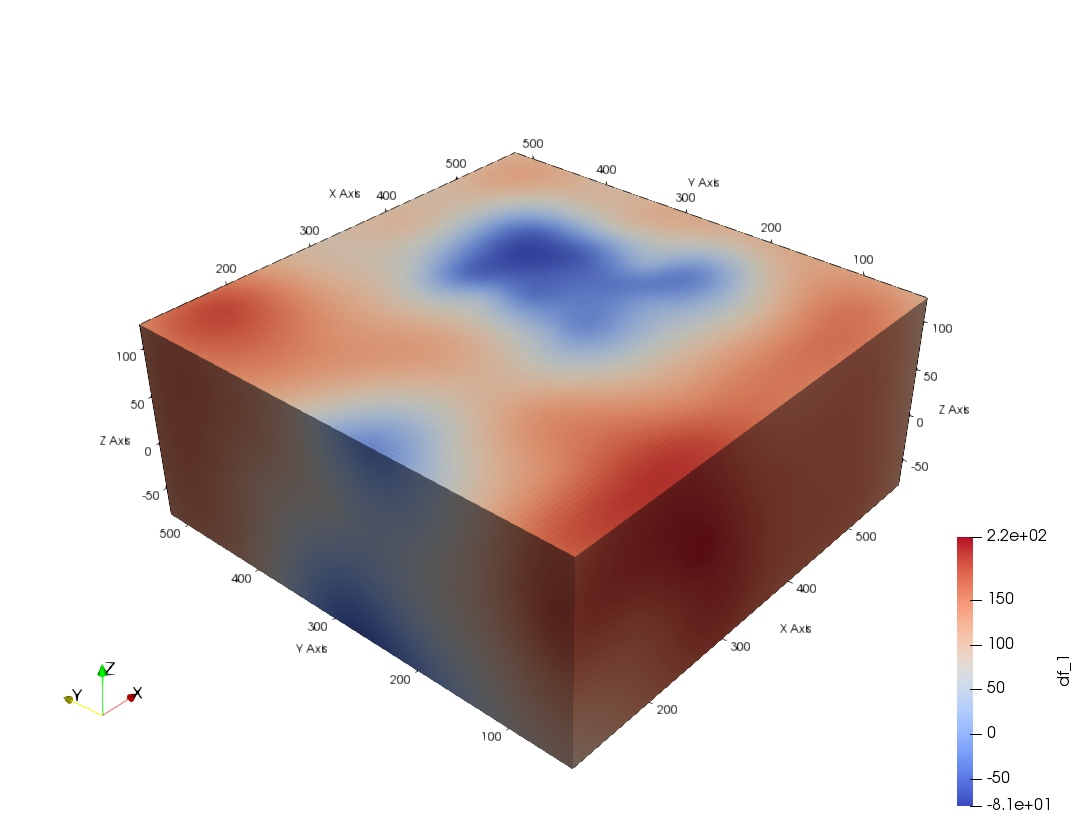
\includegraphics[width=.3\textwidth]{capitulo_2/rbf.jpeg}\label{<figure2>}}
\end{figure}

É evidente a presença de artefatos nos dois primeiros modelos. As funções de bases radiais criam um modelo suave e livre de artefatos. 

A \autoref{bench} mostra um \textit{Benchmark} dos diferentes métodos de interpolação. Todos os algoritmos utilizados são da biblioteca GSLib e foram executados em um core i7 7700HQ @ 2.8 GHz com 16 Gb de RAM.

O algoritmo de krigagem global não terminou de estimar os quase um milhão de blocos do grid fino sem terminar com uma mensagem de erro. A krigagem ordinária com 100 amostras leva 45 minutos contra pouco mais de um minuto do RBF, subdividindo o problema, é possível reduzir o tempo de interpolação para 16 segundos. Não é difícil perceber porque o RBF é o interpolador preferido na modelagem geológica implícita. O software comercial Leapfrog \textsuperscript{\textregistered} tem um algoritmo patenteado de RBF ainda mais rápido.

\begin{table}[H]
\centering
\resizebox{\textwidth}{!}{%
\begin{tabular}{lllll}
Método & Tempo grid grosso & Tempo grid fino & Classificação errônea grosso & Classificação errônea fino \\ \hline
krigagem global isotrópica & 28min &  & 121 &  \\
krigagem global anisotrópica & 30min 34s &  & 282 &  \\
krigagem ordinária anisotrópica (40) & 1min 3s & 38min & 137 & 135 \\
krigagem ordinária anisotrópica (100) &  & 45min 51s &  & 181 \\
RBF isotrópico & 21.5s &  & 57 &  \\
RBF anisotrópico &  & 1min 22s &  & 38 \\
POU RBF anisotrópico &  & 1min 2s &  & 39 \\
POU RBF artefatos & 16.5s &  &  & 29 \\
LVA OK &  &  & 8 &  \\
LVA RBF &  &  &  & 8 \\
Krigagem dos indicadores &  & 33min 27s &  & 2 \\ \hline
\end{tabular}%
}
\caption{\textit{Benchmark} dos diferentes métodos de interpolação.} \label{bench}
\end{table}

\subsection{Funções de bases radiais - RBF}

A demonstração detalhada das equações e considerações  pode ser encontrada em \citeonline{martin_boisvert_review_rbf}. Os interpoladores baseados em funções de bases radiais são globais e não necessitam de um grid. Os pesos são treinados baseados nos valores da função distância assinalada calculados para cada ponto amostral. Com os pesos treinados o valor interpolado da função distância assinalada pode ser obtido rapidamente para qualquer localização do depósito. Esse procedimento permite treinar o sistema linear de equações antes de escolher o grid de interpolação \cite{martin2017implicitmodeling}.

\subsubsection{O \textit{kernel}}

O \textit{kernel} radial estabelece as relações espacias entre todos os pontos do domínio. O \textit{kernel} 
é sinônimo a função covariância usada na krigagem, e pode/deve ser parametrizado a partir do variograma, calculado e modelado a partir das amostras. Para modelagem geológica o \textit{kernel} Gaussiano, representado pela \autoref{gauss_kernel}, é o mais indicado. Na prática tanto o variograma das funções distância assinaladas: que são modelados com um pequeno efeito pepita (para evitar instabilidades matemáticas e/ou controlar o ruído do modelo) e estrutura Gaussiana, quanto o variograma dos indicadores: que é modelado com uma estrutura esférica \cite{martin2017implicitmodeling}, são adequados para a parametrização do \textit{kernel}. Os programas da biblioteca GSLib trabalham apenas com uma única estrutura. 

\begin{equation}\label{gauss_kernel}
  \phi(r)=exp^{-\epsilon^{-2}r^2}  
\end{equation}

Onde $\epsilon$ é o parâmetro de suporte, que defino o "range" do \textit{kernel}.

Para parametrizar as funções de bases radiais com o modelo de variograma (das distâncias ou indicadores) a distância de suporte do kernel pode ser estimada a partir do alcance na direção de maior continuidade do variograma análogo. Os ângulos e relações de anisotropia são parametrizados a partir da orientação e alcances dos variogramas análogos (azimuth, dip, rake, $r1 = \frac{a_{hmin}}{a_{hmax}}$, $r2 = \frac{a_{vert}}{a_{hmax}}$).

\citeonline{fasshauer2007meshfree} advoga que o \textit{kernel} pode ser parametrizado pela distância que representa a maior esfera que pode ser colocada entre amostras no domínio. Para modelagem geológica essa técnica tende a super estimar o suporte \cite{martin2017implicitmodeling}.

\subsubsection{Decomposição do domínio} \label{dom_decomp}

Como abordado na \autoref{met_int}: a limitação dos interpoladores globais são bancos de dados volumosos. Existem algumas técnicas para superar essa limitação como a solução iterativa \cite{beatson1999fast} por exemplo. Porém, um método que apresenta resultados satisfatórios e está presente na biblioteca GSLib é a decomposição do domínio (\textit{Partition of unity - POU}) \cite{wendland2004scattered}, que transforma um problema volumoso e que demanda muito esforço computacional em diversos problemas menores e eficientes que são, ao final, unidos.

A demonstração das equações e pode ser encontrada em \citeonline{wendland2004scattered} e \citeonline{martin_boisvert_review_rbf}. Um domínio $A$ é subdividido em uma série de partições sobrepostas $\beta$ de modo que a união de todas as $k$ partições em $A$, $\{ \beta \}^K_{j=1}$ compreende o domínio. Para cada partição, os dados correspondentes são utilizados interpolar a função escalar $s_j(x)$.

A função peso para cada partição deve ser igual a um no centro e 0 na fronteira, a contribuição de cada partição nos locais de sobreposição é dado pela função peso.

As partições são definidas encontrando uma série de coordenadas para os centros. Diversos métodos podem ser utilizados: um grid regular, k-means, árvore binária, \textit{oct tree}.

\begin{figure}[H]
	\caption{\label{pou}Particionamento.}
	\begin{center}
		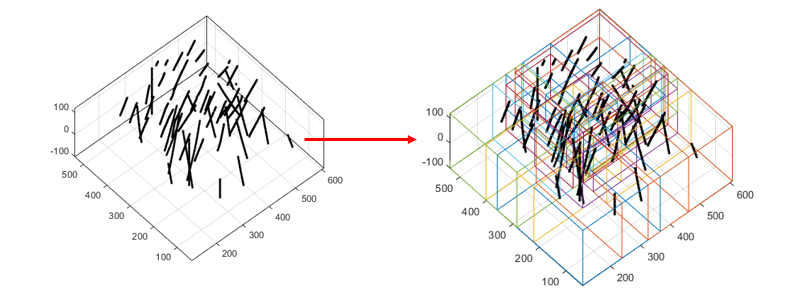
\includegraphics[width=0.7\textwidth]{capitulo_2/pou.jpg}
	\end{center}
	\legend{Fonte: \citeonline{martin_boisvert_review_rbf}}
\end{figure}

A \autoref{pou} mostra um domínio particionado: o particionamento começa considerando o domínio completo como sendo uma partição, então a partição "total" é subdividida recursivamente em duas mantendo um nível de sobreposição. O particionamento termina quando cada partição individual tem menos amostras que o máximo especificado pelo usuário \cite{martin2017implicitmodeling}. Dessa forma áreas com alta densidade amostral ficam em partições pequenas enquanto áreas esparsas ocupam partições maiores.

Deve haver um número de amostras em cada partição e sobreposição das partições suficientes para evitar o surgimento de artefatos quando as partições independentes forem unidas.

\section{Visualização do modelo geológico}

Como as funções distância são negativas no interior do domínio e positivas no exterior, um bom palpite inicial para a interface que separa os domínios no espaço, seria a linha (em duas dimensões) ou superfície (em três dimensões) que corresponda ao valor zero da função distância assinalada \cite{wildedeutschcalibrate}. 

A \autoref{isosup} mostra a iso superfície que representa a categoria 1, extraída no software Paraview, dos diferentes modelos implícitos da \autoref{interpo}. O algoritmo de extração de iso superfícies mais comumente utilizado é o dos cubos marchantes \cite{lorensen1987marching}. 

Note que os artefatos gerados nos modelos implícitos quando as distâncias foram interpoladas por krigagem são transferidos para as respectivas iso superfícies. Daí a importância de gerar modelos implícitos livres de artefatos.


\begin{figure}[H]
    \caption{Iso superfícies para a categoria 1 extraída dos diferentes modelos implícitos.} \label{isosup}
     \centering
     \subfloat[][OK com 40 amostras]{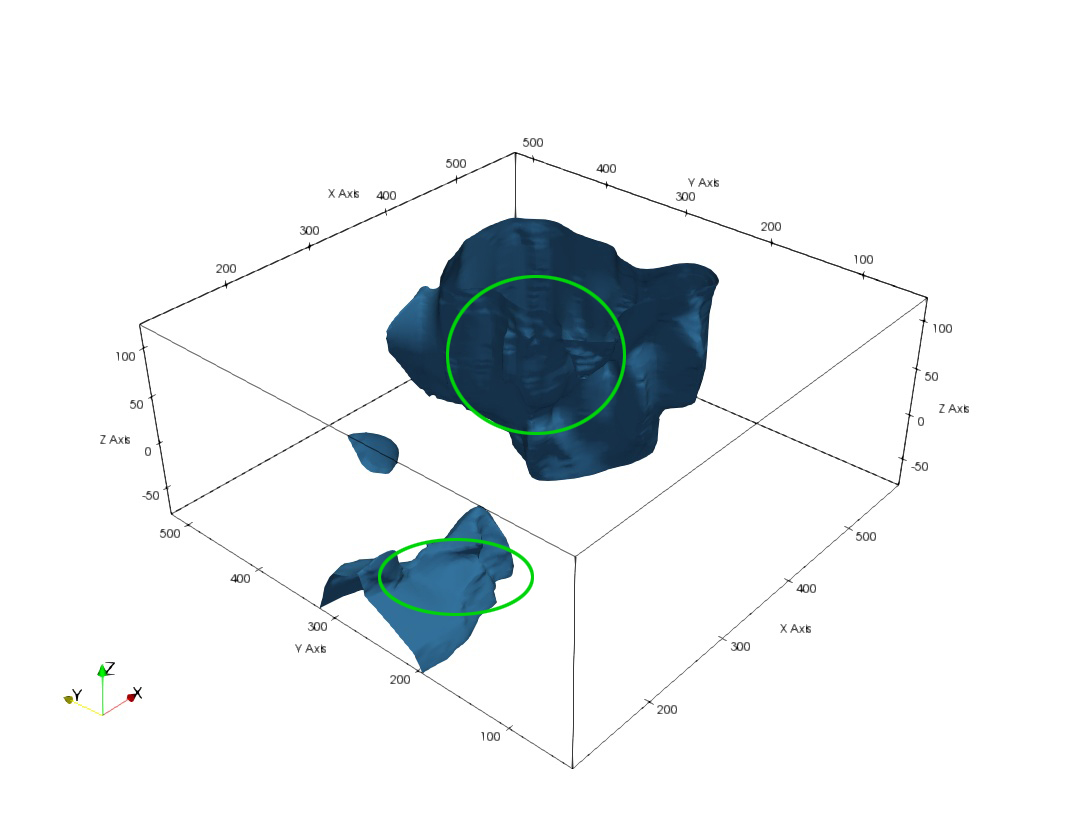
\includegraphics[width=.3\textwidth]{capitulo_2/isokt3d40.jpeg}\label{<figure1>}}
     \subfloat[][OK com 100 amostras]{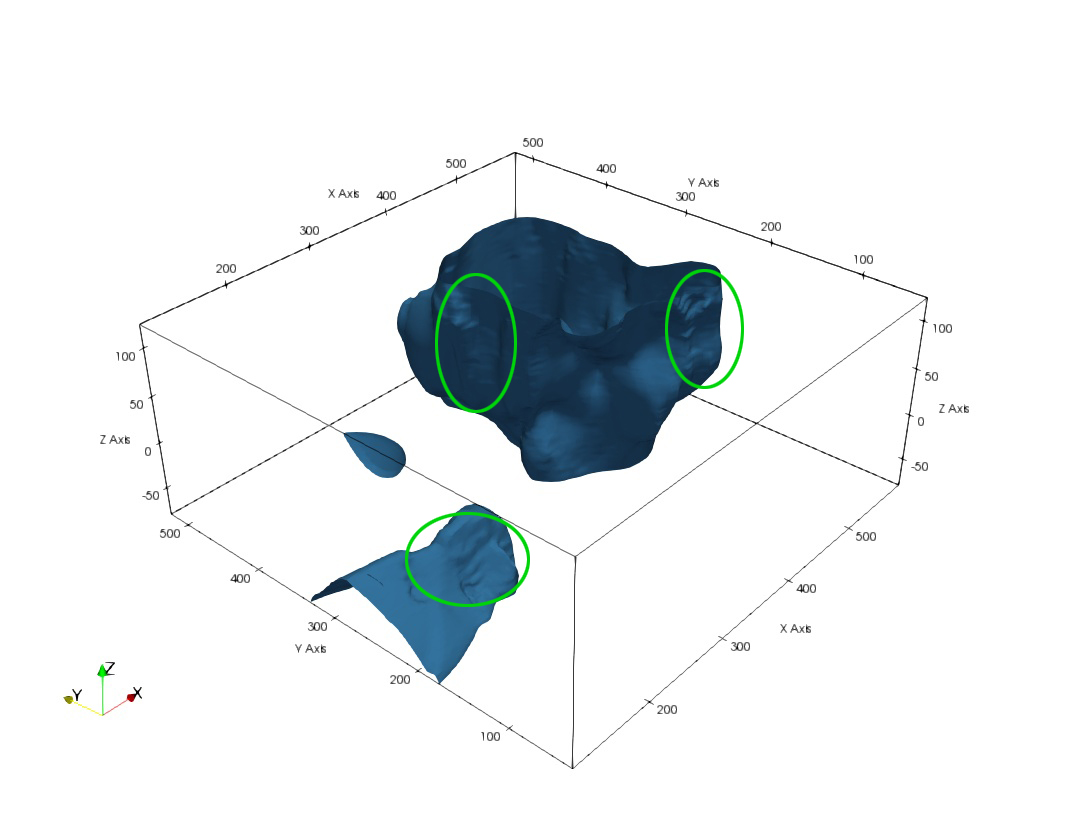
\includegraphics[width=.3\textwidth]{capitulo_2/isokt3dn100.jpeg}\label{<figure2>}}
     \subfloat[][RBF global]{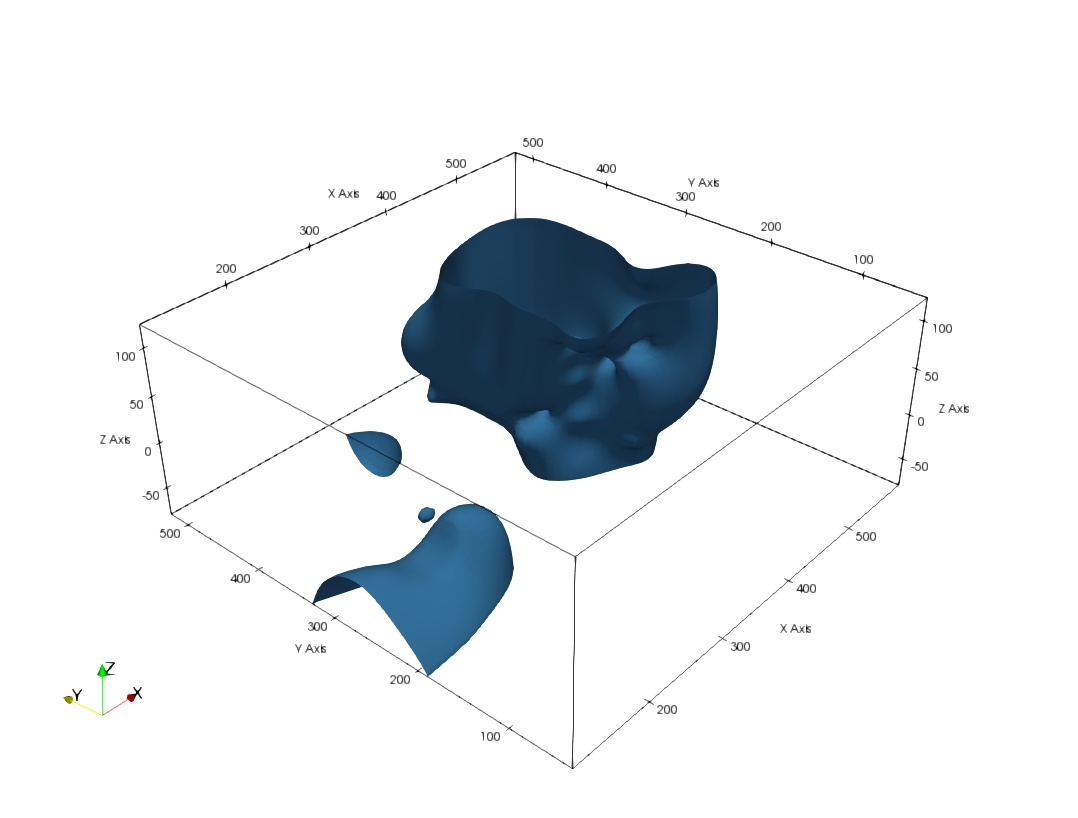
\includegraphics[width=.3\textwidth]{capitulo_2/isorbf.jpeg}\label{<figure2>}}
\end{figure}

Na presença de múltiplos domínios as iso superfícies devem ser extraídas uma a uma e algum tipo de regra hierárquica baseada na idade de cada litologia deve ser aplicada para a criação dos modelos multi categóricos.

As \autoref{iso_cat1} e \autoref{iso_cat2} mostram iso superfícies extraídas dos modelos implícitos interpolados por RBF e parametrizados a partir do variograma dos indicadores juntamente com as amostras categóricas no grid fino. 

\begin{figure}[H]
    \caption{Iso superfície extraída do modelo implícito interpolado por RBF para a categoria 1.} \label{iso_cat1}
     \centering
     \subfloat[][Vista 1]{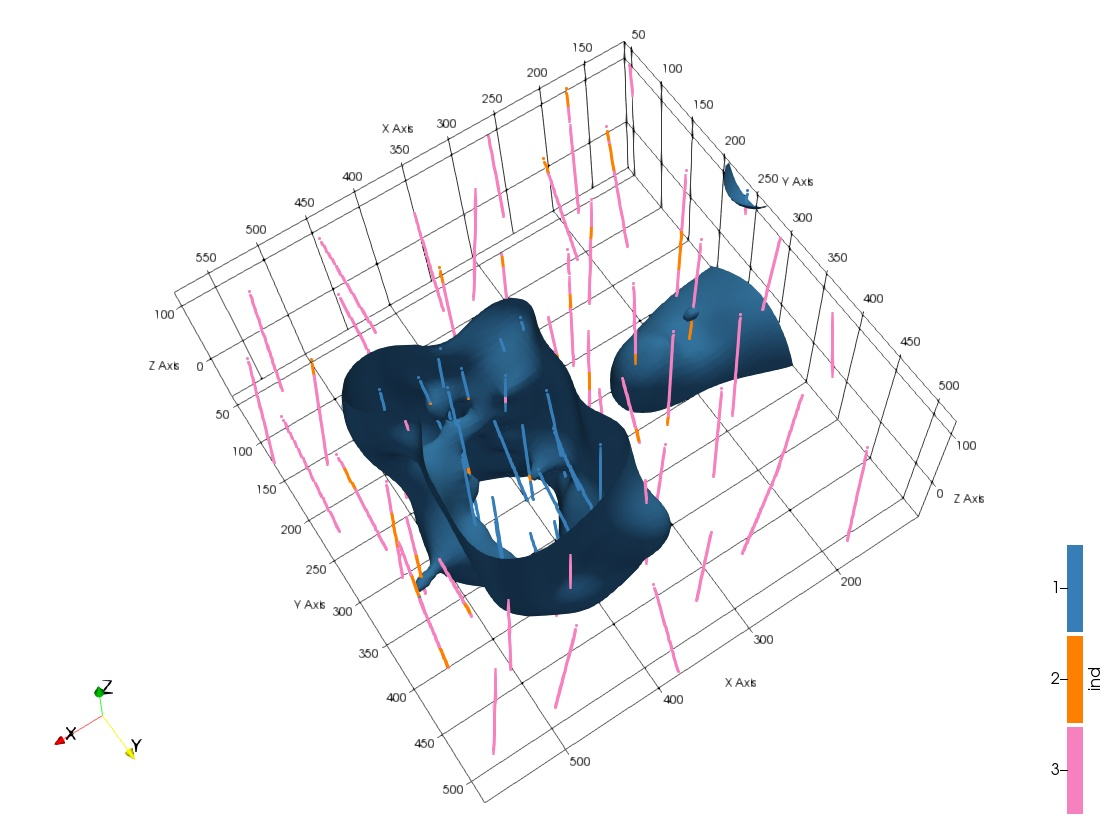
\includegraphics[width=.5\textwidth]{capitulo_2/iso_cat1_rbf.jpeg}\label{<figure1>}}
     \subfloat[][Vista 2]{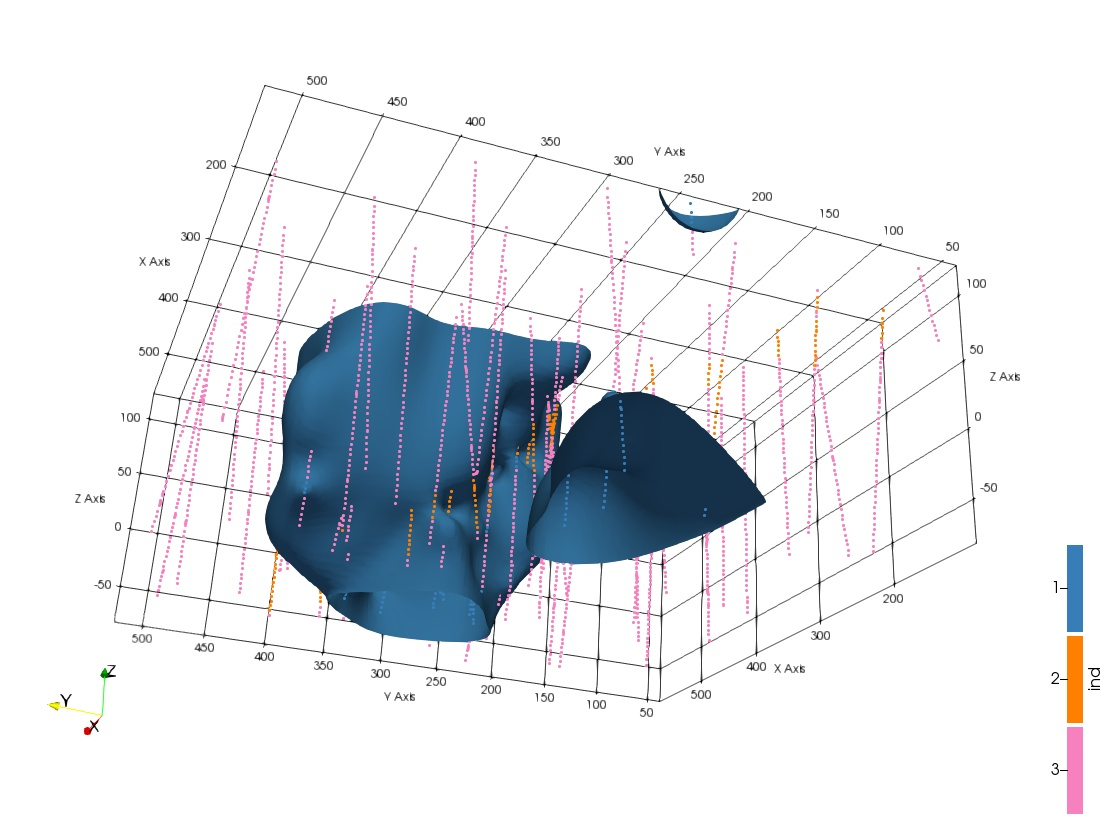
\includegraphics[width=.5\textwidth]{capitulo_2/iso_cat1_rbf2.jpeg}\label{<figure2>}}
\end{figure}

\begin{figure}[H] 
    \caption{Iso superfície extraída do modelo implícito interpolado por RBF para a categoria 2.} \label{iso_cat2}
     \centering
     \subfloat[][Vista 1]{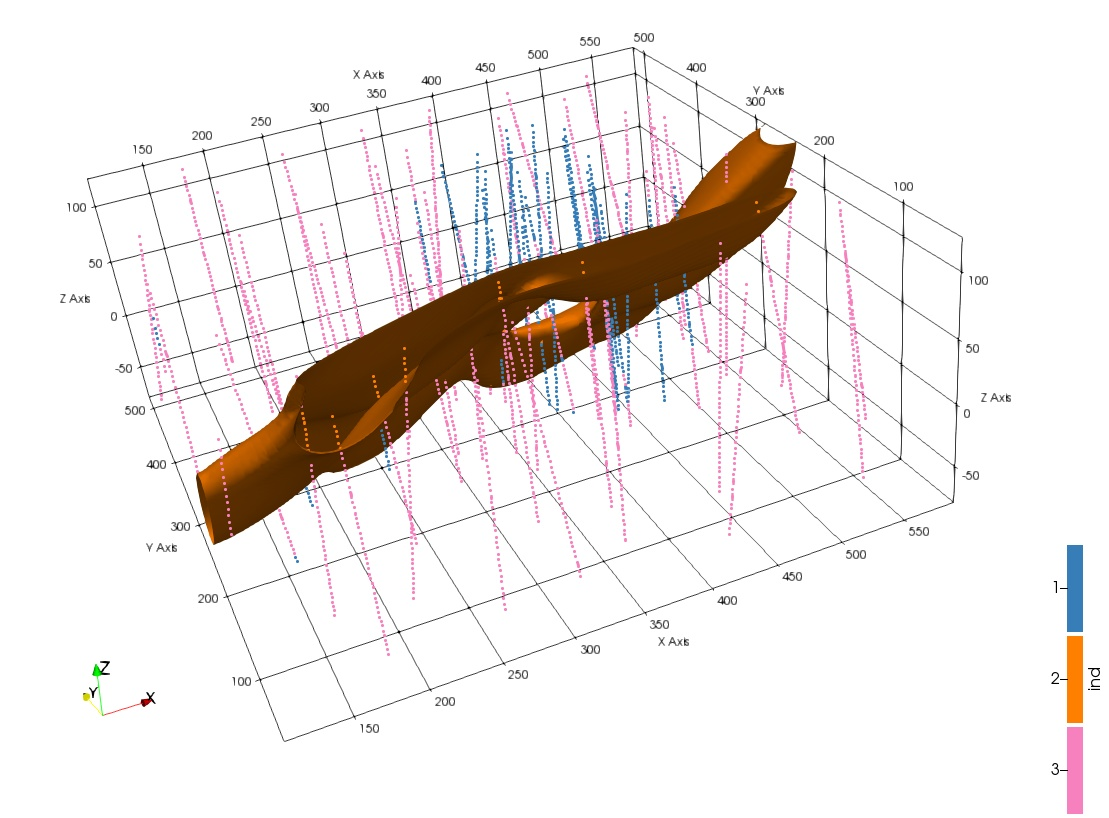
\includegraphics[width=.5\textwidth]{capitulo_2/iso_cat2_rbf.jpeg}\label{<figure1>}}
     \subfloat[][Vista 2]{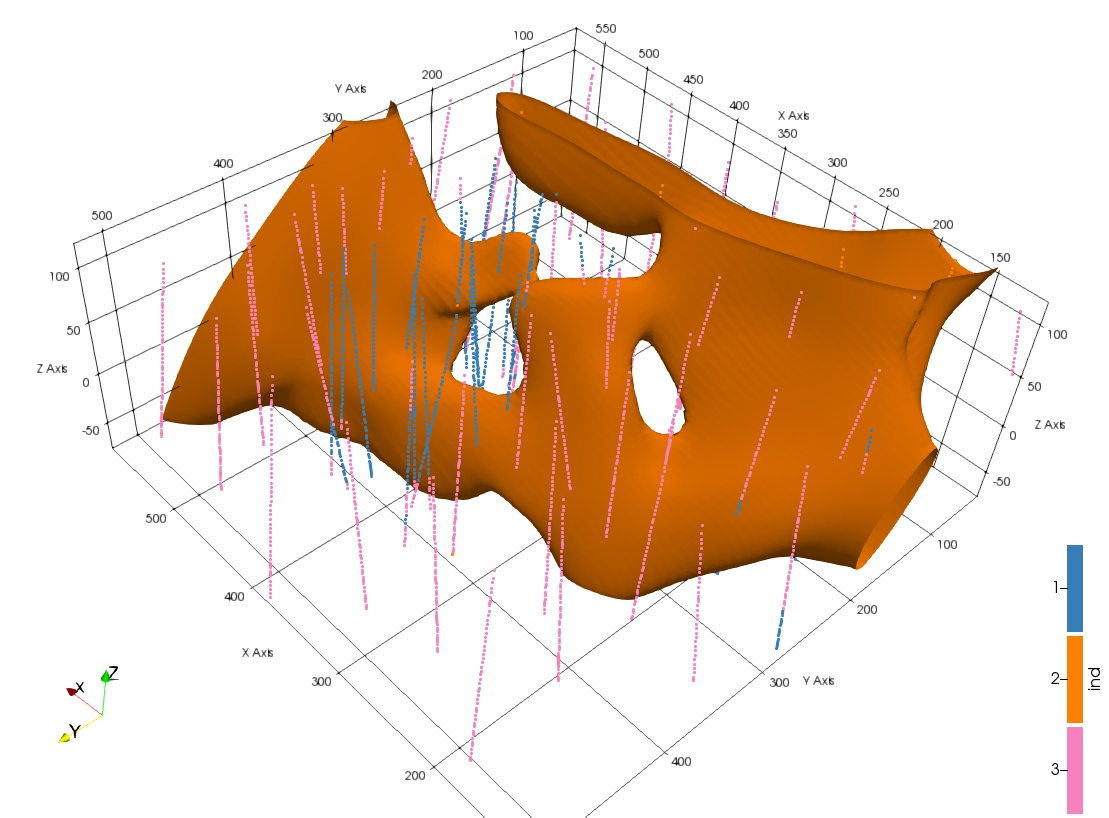
\includegraphics[width=.5\textwidth]{capitulo_2/iso_cat2_rbr2.jpeg}\label{<figure2>}}
\end{figure}

\subsection{Adaptação do método para múltiplas categorias simultâneas}\label{multi_cat}

\citeonline{silvaanddeutschccgmodeling} propuseram, uma adaptação para o método com o objetivo de modelar múltiplos domínios geológicos simultaneamente, de forma similar ao caso binário.

Se existirem $K$ múltiplos domínios no depósito mineral, para cada ponto amostral ${z(u_\alpha),\alpha=1,...,n}$, um vetor de indicadores de $K$ elementos é codificado de acordo com a \autoref{eq_mult_ind}.

\begin{equation}
	i_k(u_\alpha)=\begin{cases}
	1,\:\textrm{se}\:z(u_\alpha)=k\\
    0,\:\textrm{se}\:z(u_\alpha)\:\textrm{caso contrário}\end{cases} k=1,...,K
    \label{eq_mult_ind}
\end{equation}

A função distância é calculada, individualmente para cada elemento $k$ do vetor, de acordo com a \autoref{eq_mult_sg}.

\begin{equation}
	d_k(u_\alpha)=\begin{cases}
	-\parallel u_\alpha-u_\beta\parallel,\:\textrm{se}\:i_k(u_\alpha)=1\\
	+\parallel u_\alpha-u_\beta\parallel,\:\textrm{se}\:i_k(u_\alpha)=0\end{cases} k=1,...,K
    \label{eq_mult_sg}
\end{equation}

As distâncias calculadas são então interpoladas pelo método escolhido, individualmente para todos os nós do grid de acordo com a \autoref{eq_mult_ok}.

\begin{equation}
	d_k^*(u)=\sum\limits_{\alpha=1}^n \lambda_\alpha(u)d_k(u_\alpha)\quad k=1,...,K
    \label{eq_mult_ok}
\end{equation}

Por fim, cada bloco é  classificado pela \autoref{eq_mult_rt}

\begin{equation}
	i^*(u)=k'\;\text{de modo que}\;d_{k'}^*=min\{d_k^*(u)\}_{k=1}^K
    \label{eq_mult_rt}
\end{equation}

As distâncias estimadas fornecem uma medida de proximidade ao domínio oposto mais próximo. Sendo assim, a mínima distância assinalada estimada é tida como o domínio mais provável de ser encontrado numa região não amostrada. A \autoref{eq_mult_rt} sumariza essa ideia \cite{silvaenhancedgeomodeling}. A categoria associada com a menor distância estimada é retida em cada bloco.

A \autoref{mult_cat} mostra um exemplo de um modelo geológico criado a partir da mínima distância assinalada estimada. A esquerda, a figura mostra a projeção das distâncias assinaladas para cada uma das quatro categorias, e à direita a classificação final.

\begin{figure}[H]
    \caption{\label{mult_cat}Esquema para criação de um modelo implícito multi categórico.}
	\begin{center}
		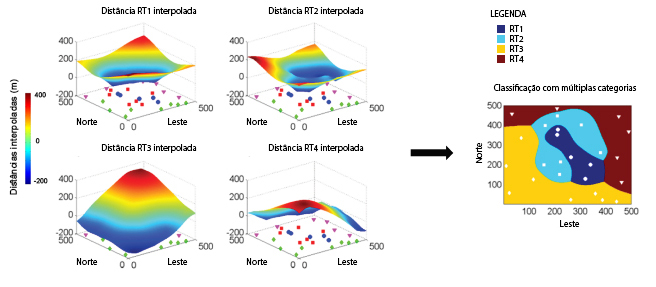
\includegraphics[width=0.8\textwidth]{capitulo_2/mult_cat_legenda.jpg}
	\end{center}
	\legend{Fonte: Modificado de \citeonline{silvageostatlessons}}
\end{figure}

A \autoref{multi_cat_rbf} mostra seções verticais em XZ e YZ de um modelo geológico implícito multi categórico criado por RBF parametrizado pelo variograma dos indicadores para o banco de dados do estudo de caso no grid fino. Nas seções também são mostradas amostras a 3 metros do centroide dos blocos na direção X e Y.

\begin{figure}[H]
\caption{Modelo geológico multi categórico} 
\label{multi_cat_rbf}
\begin{center}
\subfloat[][Seções em XZ do modelo implícito gerado por RBF no grid fino.]{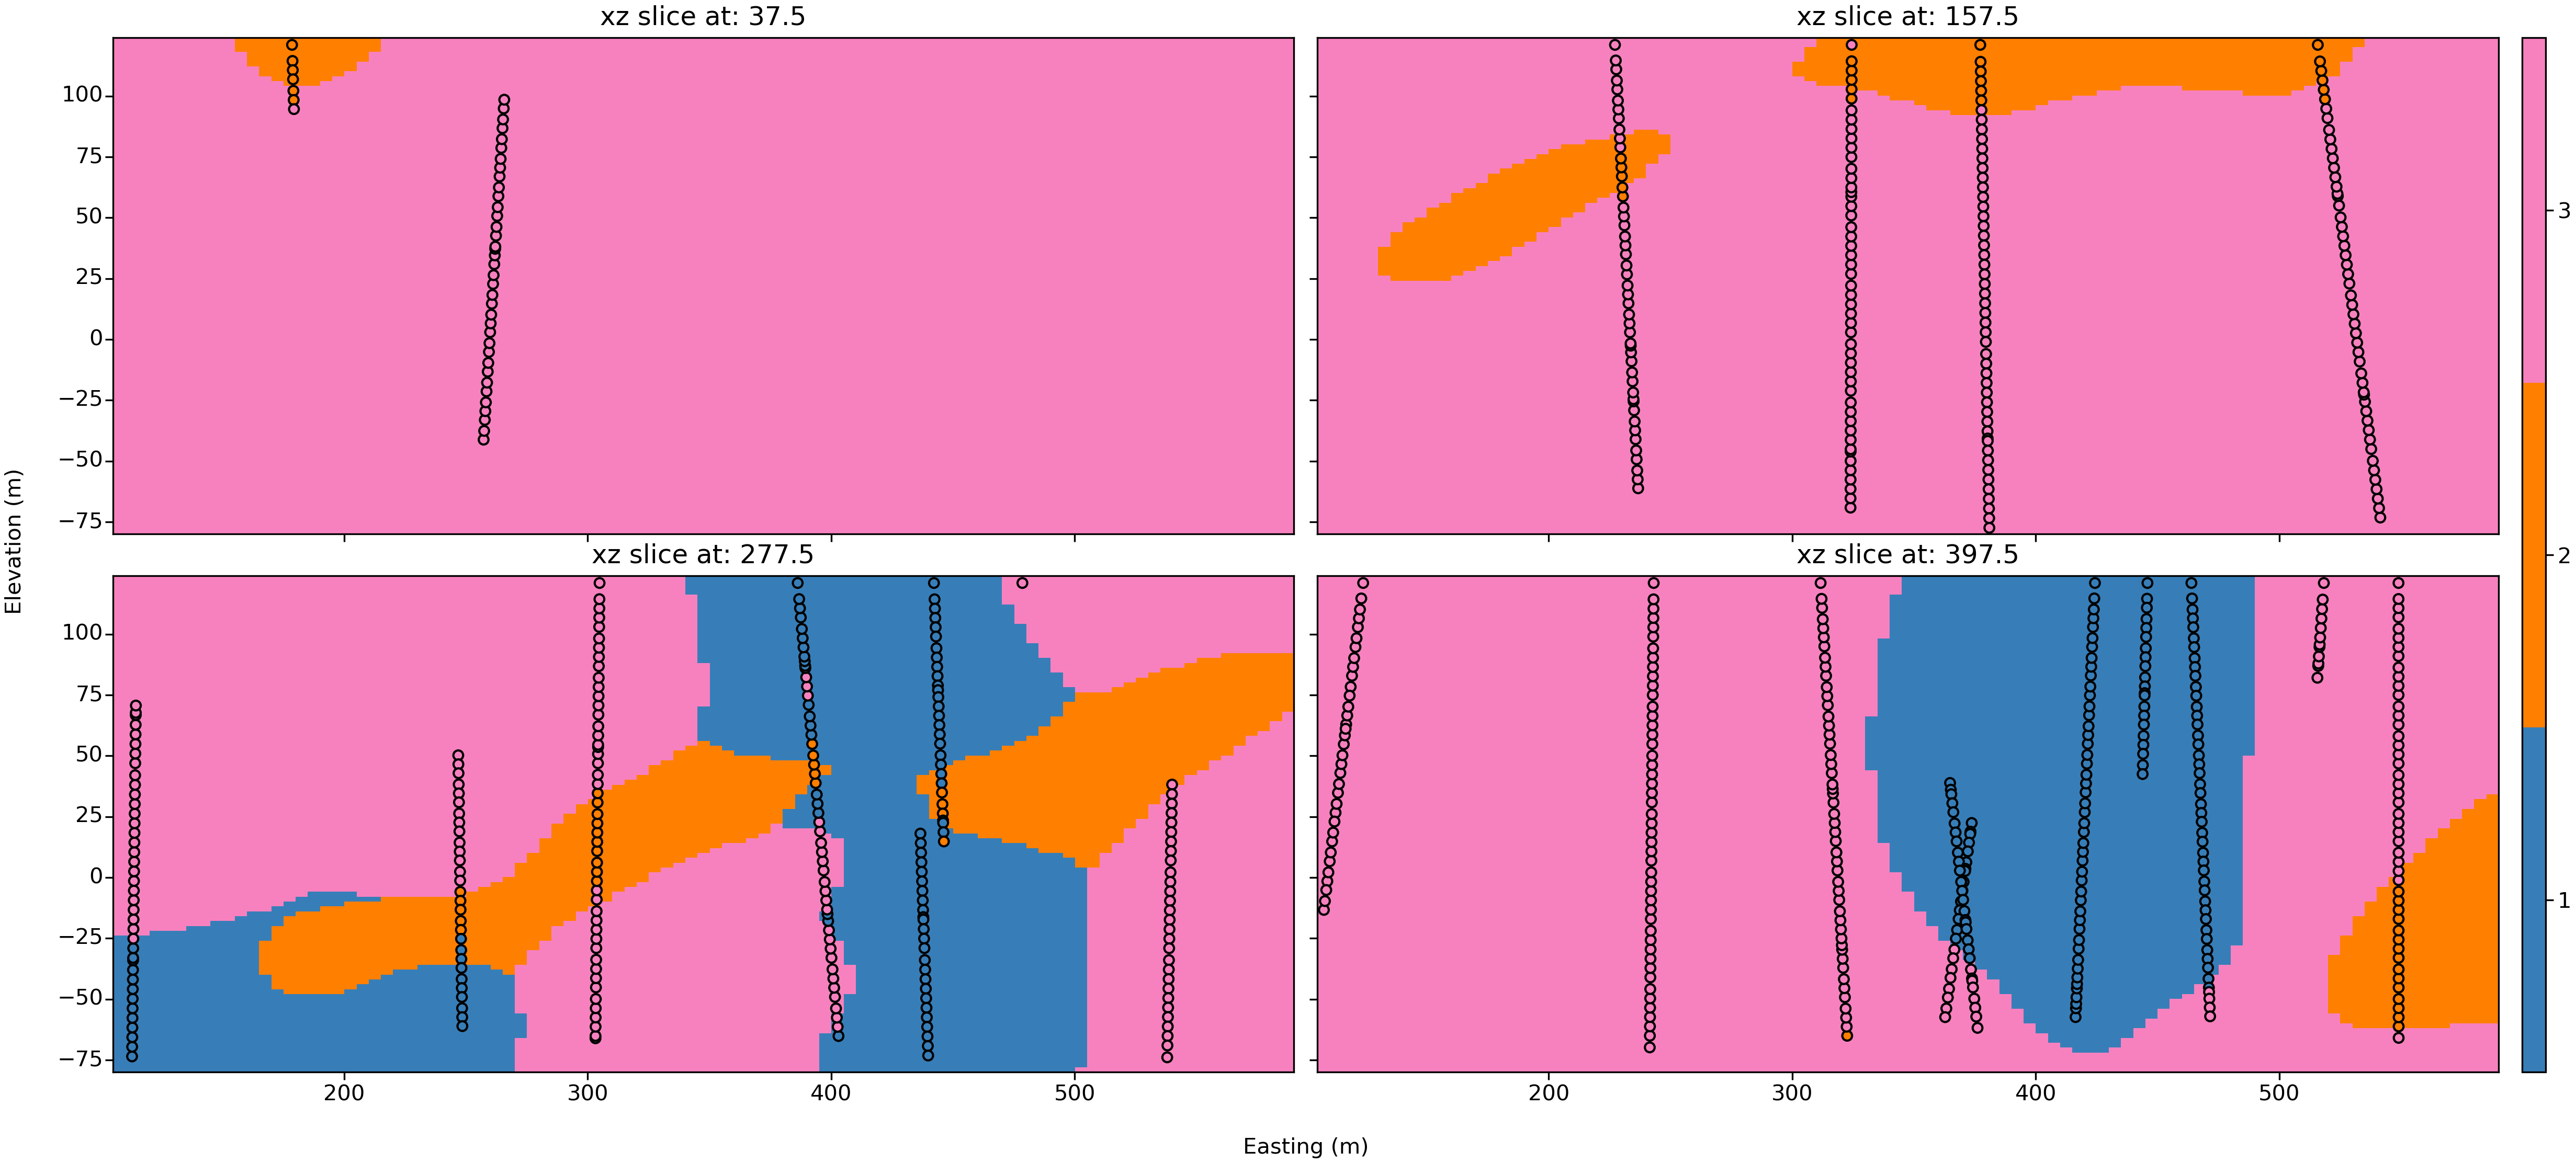
\includegraphics[width=0.8\textwidth]{capitulo_2/anisofinexz.png}\label{a}}\\
\end{center}
\begin{center}
\subfloat[][Seções em YZ do modelo implícito gerado por RBF no grid fino.]{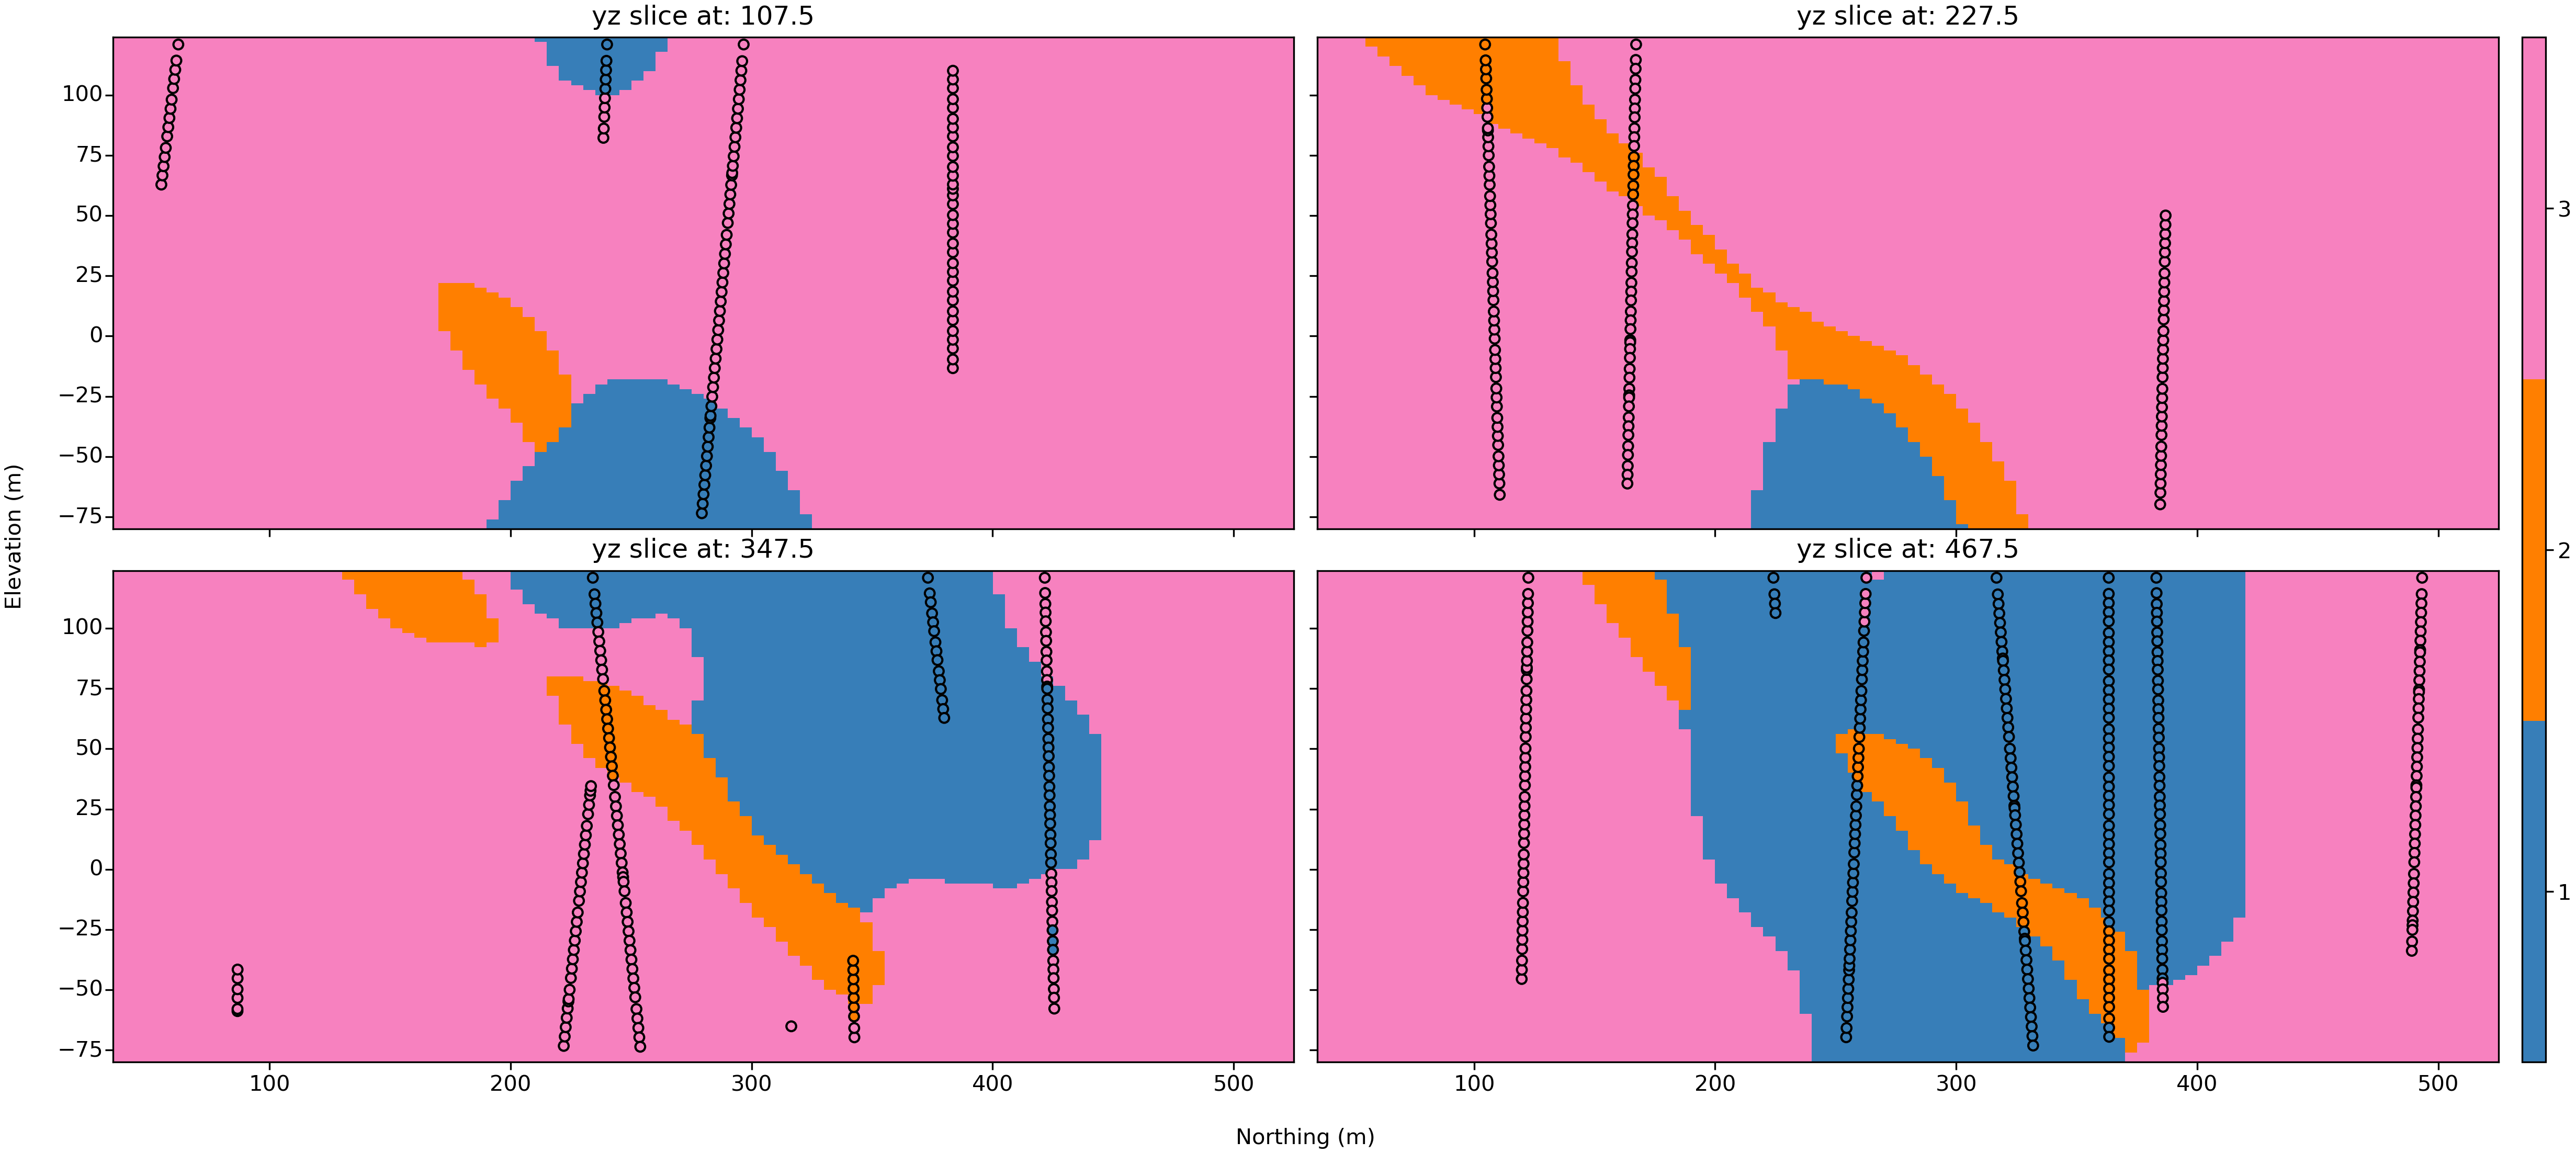
\includegraphics[width=0.8\textwidth]{capitulo_2/anisofineryz.png}\label{b}}
\end{center}
\end{figure}

A variação do método para múltiplos domínios ou categorias simultâneos deve ser utilizado com cautela, em muitos casos, em especial em depósitos com geologia complexa que apresentam intrusões, falhas e dobras é indicado a modelagem e análise das litologias individualmente, ou até mesmo com algum nível de interpretação geológica manual via digitalização de seções.

\section{Incorporação da não estacionariedade de segunda ordem}

Corpos geológicos são complexos da escala macro à escala micro. Essa característica pode tornar difícil a captura de suas feições com funções de covariância. Segundo \citeonline{martin2017implicitmodeling} a não estacionariedade de segunda ordem deve ser incorporada quando estruturas complexas estão sendo modeladas.

Anisotropia é definida como o conjunto de rotações e relações anisotrópicas: azimuth, dip, rake, $r1 = \frac{a_{hmin}}{a_{hmax}}$, $r2 = \frac{a_{vert}}{a_{hmax}}$. 

\subsection{Krigagem com anisotropia local variável}

A krigagem com anisotropia variável exige que os parâmetros locais de anisotropia sejam definidos em todos os nós do grid (\autoref{lva_krig_cartoon}), e variem de forma suave pelo domínio. Isso permite que estruturas curvilineares em escala menor que o espaçamento entre as amostras sejam capturadas \cite{martin2017implicitmodeling}. Porém, torna o método computacionalmente exigente.

\begin{figure}[H]
\caption{\label{lva_krig_cartoon}Esquema mostrando os vetores de anisotropia local para cada nó do grid.}
	\begin{center}
		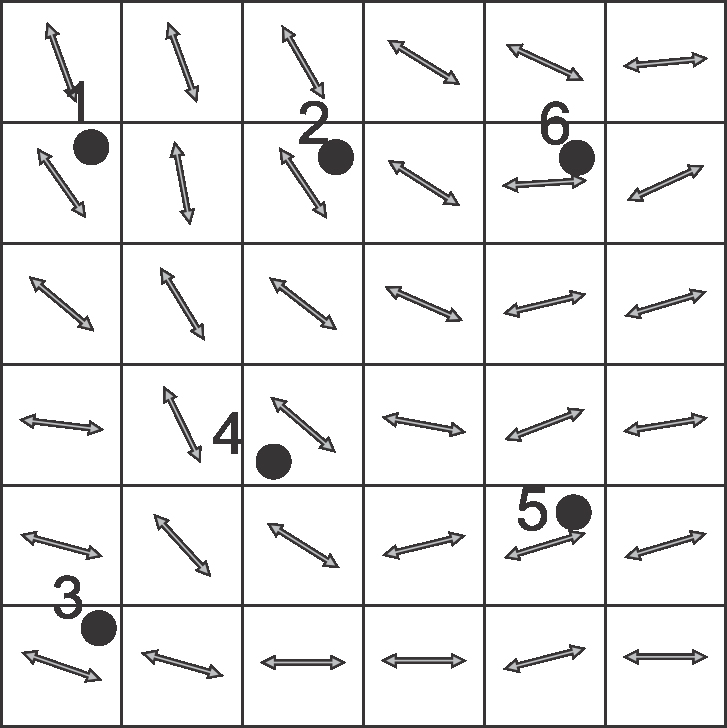
\includegraphics[width=0.3\textwidth]{capitulo_2/lvakrig.jpg}
	\end{center}
	\legend{Fonte: \citeonline{martin2017implicitmodeling}}
\end{figure}

Existem diversos métodos para definição da anisotropia local \cite{lillah2015inference}: pode ser inferida por um geomodelador, estimada diretamente a partir dos dados usando técnicas automáticas, interpolada de uma série de pontos onde a orientação foi medida ou pode ser extraída de dados em um grid que representam a variabilidade local (teores krigagdos, por exemplo). A bilioteca GSLib tem diversos softwares para definição de anisotropia local. 

A \autoref{lva_krig} mostra a iso superfície para a categoria 1 extraída de um modelo implícito gerado por krigagem com anisotropia local variável. Os vetores de anisotropia são plotados e foram gerados pelo software \verb|imorient| da biblioteca GSLib a partir de um modelo implícito para a categoria 1 previamente interpolado. A interpolação foi feita no grid grosso, a condição da anisotropia local para cada nó do grid torna o algoritmo computacionalmente exigente.

Esse programa analisa uma janela centrada em cada nó e estima a orientação dominante nessa janela, uma janela pequena captura variações em menor escala e uma janela grande variação de larga escala. É preciso encontrar um balanço \cite{lillah2015inference}.

\begin{figure}[H] 
\caption{Iso superfície para a categoria 1 extraída de um modelo implícita gerado por krigagem com anisotropia local variável mostrando os vetores.} \label{lva_krig}
     \centering
     \subfloat[][Todos os vetores de anisotropia local]{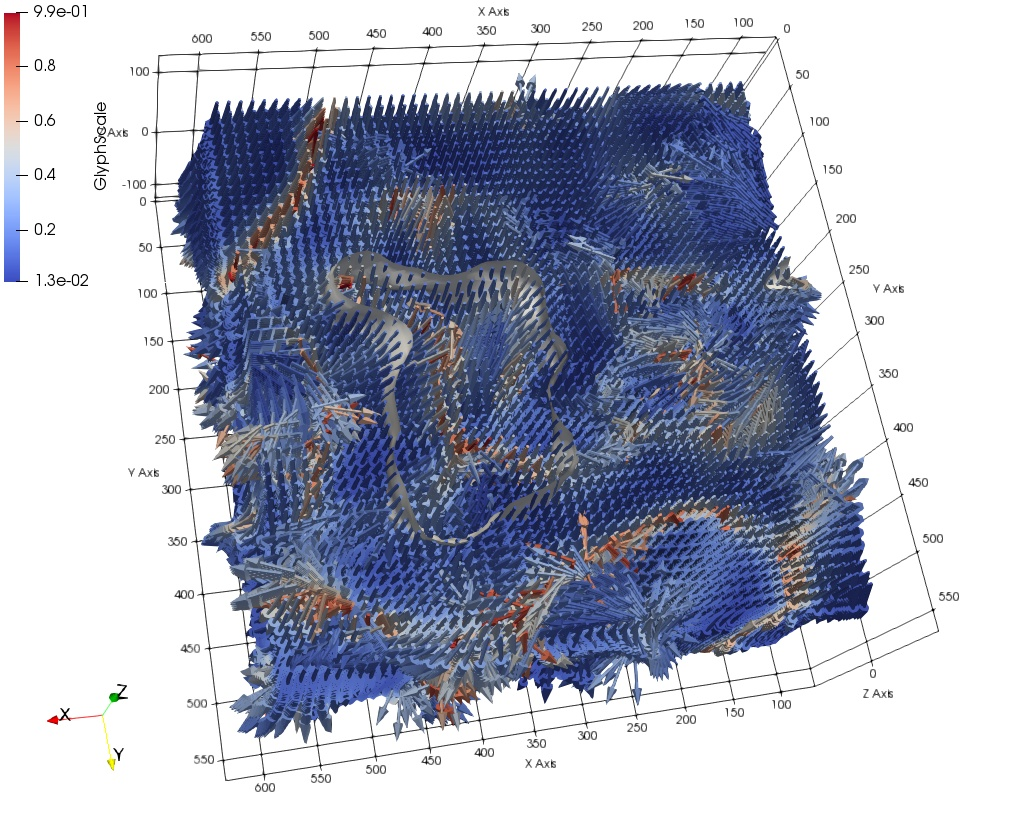
\includegraphics[width=.5\textwidth]{capitulo_2/lva_krig.jpeg}\label{<figure1>}}
     \subfloat[][Um vetor a cada 100.000 blocos]{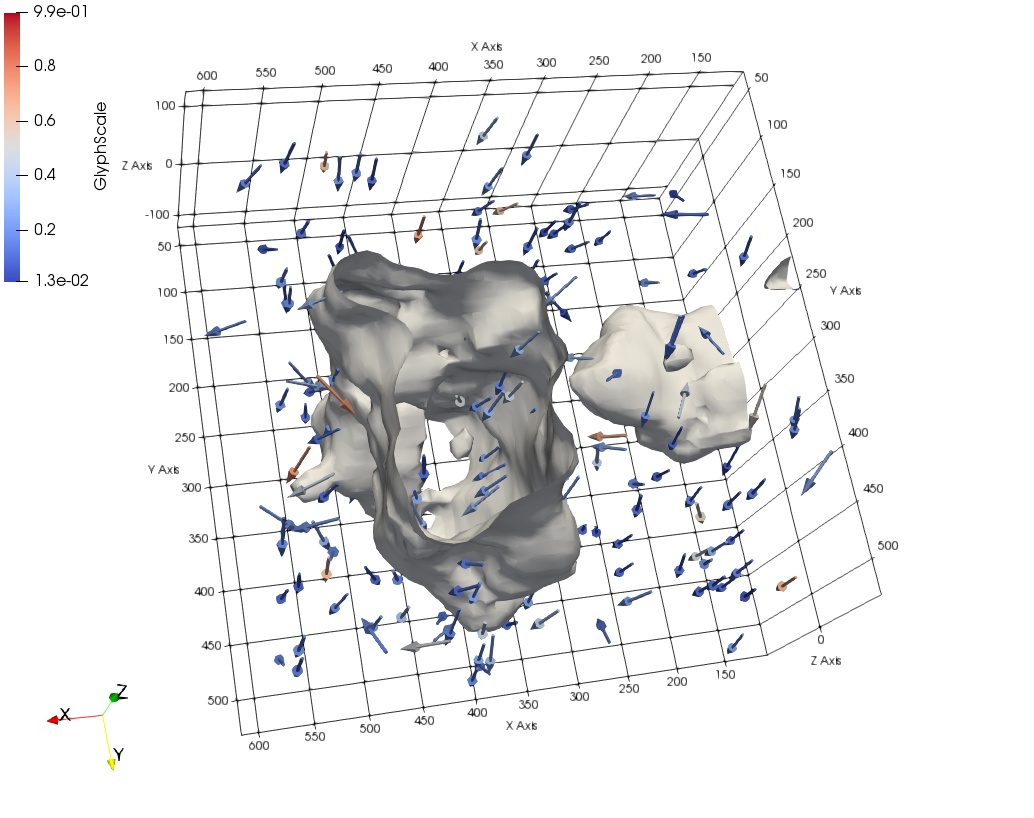
\includegraphics[width=.5\textwidth]{capitulo_2/lva_krig_100000.jpeg}\label{<figure2>}}
\end{figure}

\subsection{Funções de bases radiais com anisotropia local variável}

RBF com anisotropia local variável é baseado na decomposição de domínios (\autoref{dom_decomp}), um kernel anisotrópico pode ser usado para melhor suportar os dados em cada partição, já que as partições são independentes uma matriz de rotação é usada para definir \textit{kernels} anisotrópicos locais que melhor se ajustam às propriedades espaciais de cada partição. O interpolador de bases radiais é obtido independentemente para cada partição e a solução final é obtida ponderando as soluções independentes nos locais de sobreposição \cite{martin2017implicitmodeling}.

Ao contrário da krigagem com anisotropia local variável, que requer os vetores de anisotropia em todas os nós do grid, a implementação para funções de bases radiais requer os vetores somente no centro de cada partição (\autoref{lva_krig_cartoon}) e que variem suavemente pelo domínio.

\begin{figure}[H]
\caption{\label{lva_rbf+cartoon} Esquema mostrando os vetores de anisotropia local para cada centro de partição.}
	\begin{center}
		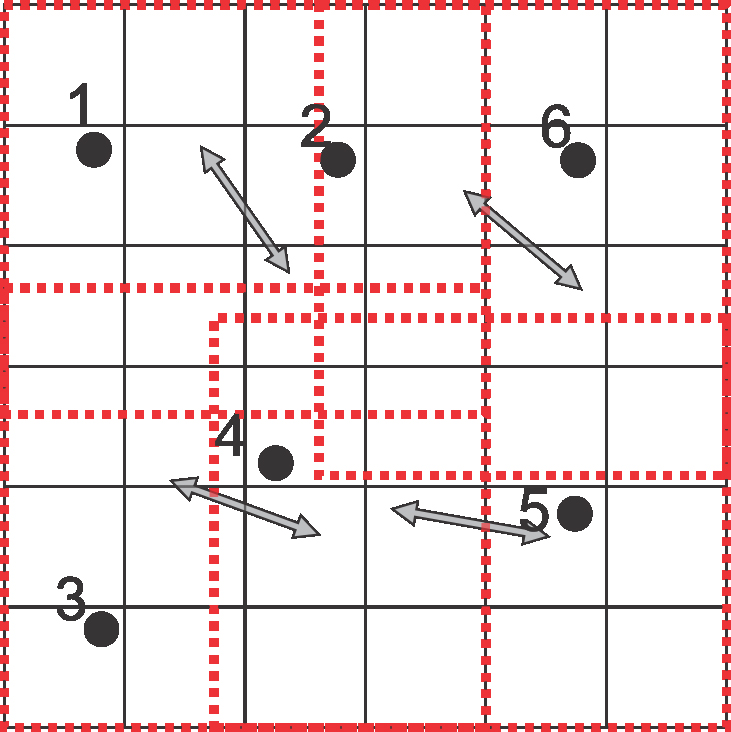
\includegraphics[width=0.3\textwidth]{capitulo_2/lvarbf.jpg}
	\end{center}
	\legend{Fonte: \citeonline{martin2017implicitmodeling}}
\end{figure}

A \autoref{rbf_iterref} mostra a iso superfície para a categoria 1 extraída de um modelo implícito gerado por funções de bases radiais com anisotropia local variável. Os vetores de anisotropia são plotados e foram gerados pelo software \verb|rbfiterref| da biblioteca GSLib. A interpolação foi feita no grid fino.

\begin{figure}[H]
\caption{\label{rbf_iterref}Iso superfície para a categoria 1 extraída de um modelo implícita gerado por krigagem com anisotropia local variável mostrando os vetores.}
	\begin{center}
		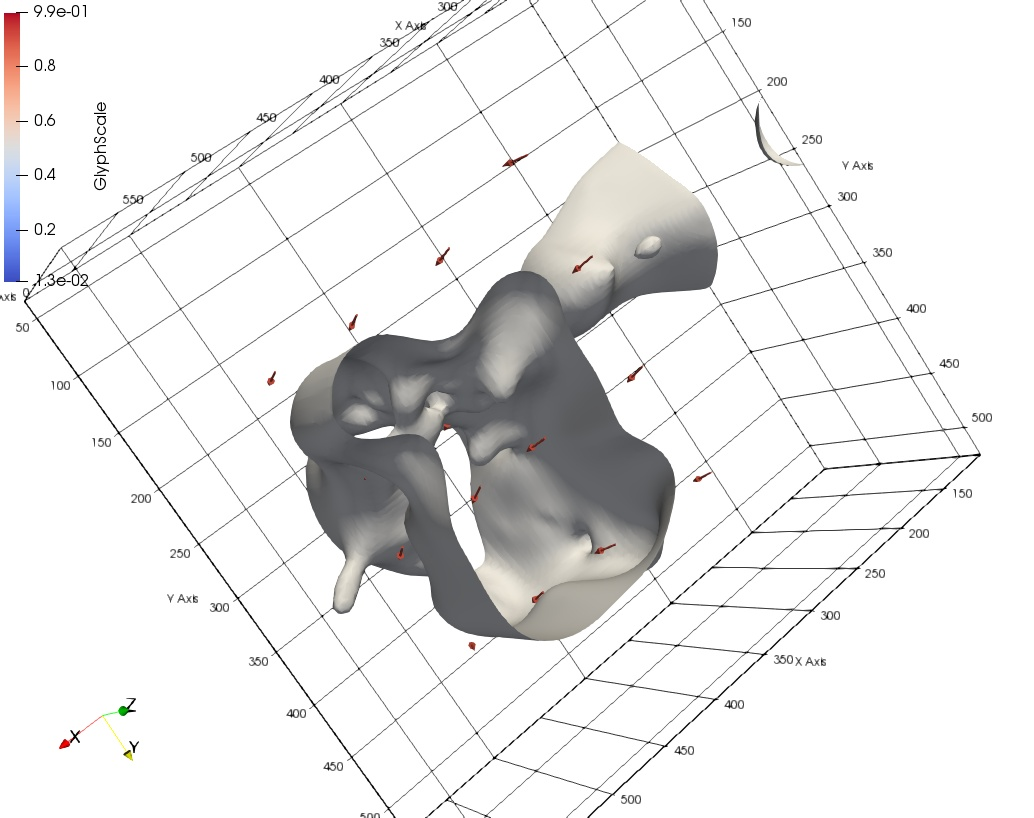
\includegraphics[width=0.5\textwidth]{capitulo_2/rbf_iterref.jpeg}
	\end{center}
	%\legend{Fonte: Modificado de \citeonline{silvageostatlessons}}
\end{figure}

\subsection{Refinamento iterativo}

Extrair orientações locais de um modelo criado com anisotropia global e utilizar essas orientações em uma nova interpolação não estacionária resulta em um modelo geológico mais refinado considerando informação local. Esse processo pode ser repetido, continuamente refinando o campo de anisotropias locais. 

O refinamento iterativo com funções de bases radiais tem um benefício extra (em relação à krigagem com variação local de anisotropia), a possibilidade de incluir algum tipo de critério de parada, quando o modelo for considerado refinado. Como as partições são independentes, se o refinamento de uma partição em particular não resultará em mudanças significativas, pode ser omitido na solução final. Essa característica torna o processo significativamente mais rápido \cite{martin2017implicitmodeling}.

A \autoref{iterref} mostra um processo de refinamento iterativo onde a semente é um modelo isotrópico. O programa \verb|rbfiterref| começa sua execução inferindo orientações anisotrópicas em cada flanco da dobra, que são rasos demais para que sejam definidos adequadamente. Porém, nas próximas iterações do refinamento o mergulho se torna mais profundo e os flancos são definidos implicitamente.

\begin{figure}[H]
\caption{\label{iterref} Esquema mostrando o refinamento iterativo para funções de bases radiais.}
	\begin{center}
		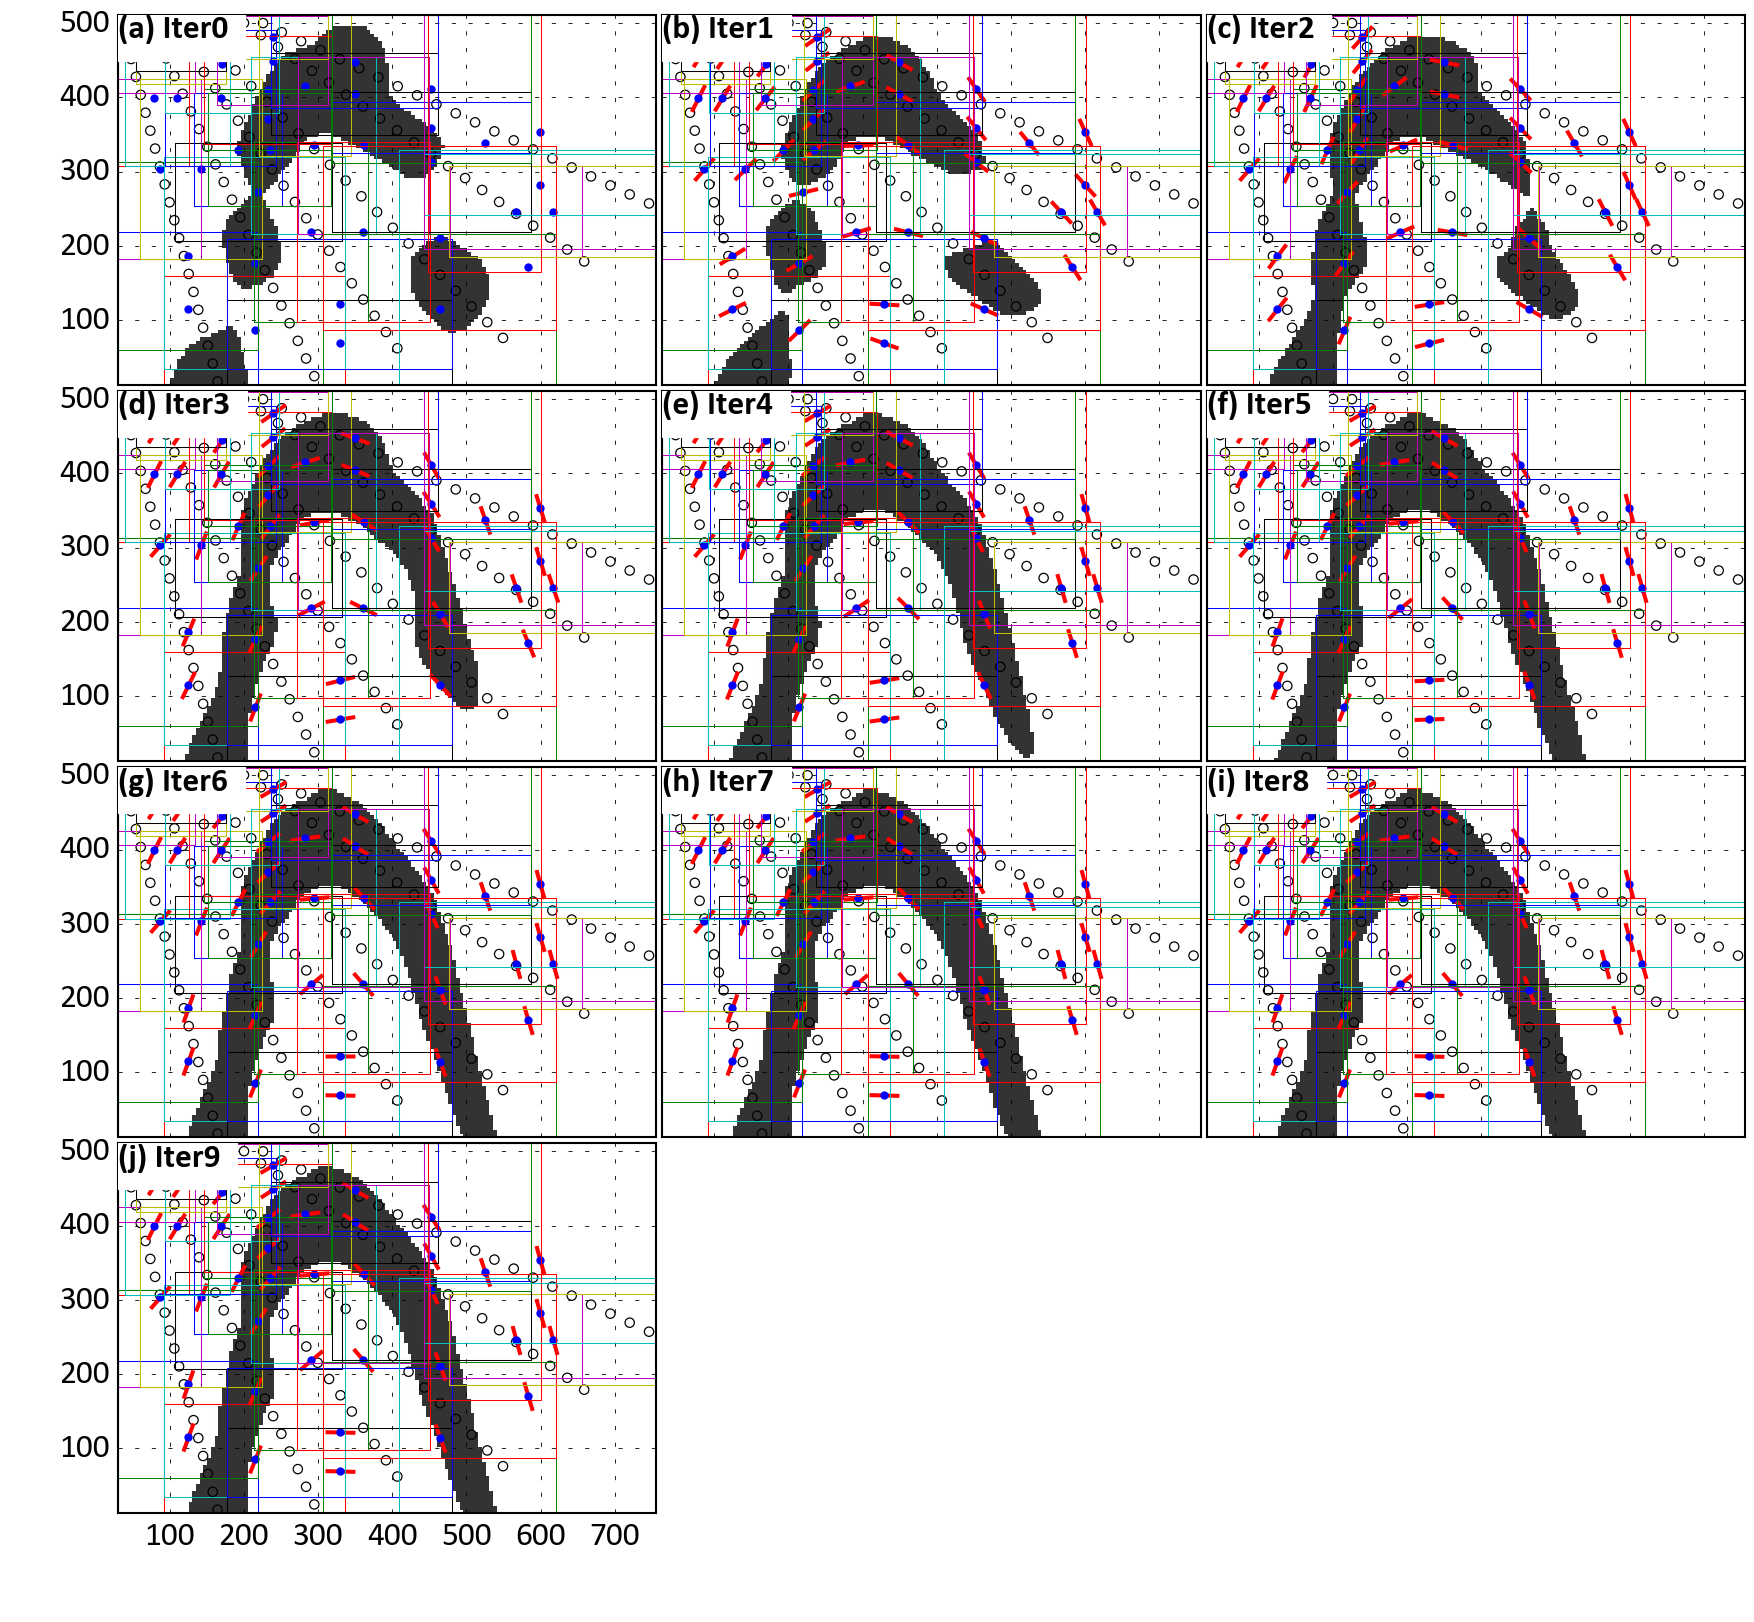
\includegraphics[width=0.7\textwidth]{capitulo_2/iterref.jpg}
	\end{center}
	\legend{Fonte: \citeonline{martin2017implicitmodeling}}
\end{figure}

\section{Incorporação de informação secundária}

Modelos explícitos englobam julgamento profissional que é difícil de superar por qualquer
algoritmo implícito devido à complexidade de representar objetos naturais com funções numéricas, principalmente quando os dados são esparsos. 

Uma desvantagem da modelagem implícita é que muitas vezes o modelo resultante não está de acordo com a interpretação e expectativa do geomodelador. Assistência humana usualmente é necessária para construir modelos geológicos semi automáticos utilizando técnicas que utilizem informação explícita e implícita  como a interpolação suave discreta (\textit{Discrete smooth interpolation - DSI}) \cite{malletgeomodeling}. Nas primeiras fases da mineração a proporção explícita da modelagem é maior, a medida que mais dados são obtidos, a proporção de intervenção humana é menor \cite{manchuck_MLS}.

O uso da krigagem ou funções de bases radiais limita os dados ao suporte puntual. \citeonline{manchuck_MLS} propõe o uso de uma regressão linear local chamada mínimos quadrados móveis (\textit{Moving least squares - MLS}) que ajusta uma função aos dados para integrar modelagem geológica implícita e explicita. MLS é um algoritmo de interpolação geral que pode ser usado para ajustar uma função em pontos, linhas e polígonos. 
MLS foi escolhido por sua capacidade de interpolar dados em linha de forma exata. Representar as linhas como pontos discretos ou utilização de integração numérica não é necessário. 

\citeonline{manchuck_MLS} conduziram um estudo de caso em um banco de dados real de ouro, o banco de dados e o resultado final podem ser vistos na \autoref{mls_model}.

\begin{figure}[H]
\caption{Modelo geológico híbrido criado a partir de furos de sondagem e seções interpretadas.}\label{mls_model}
\begin{center}
\subfloat[][Seção mostrando furos e seções interpretadas.]{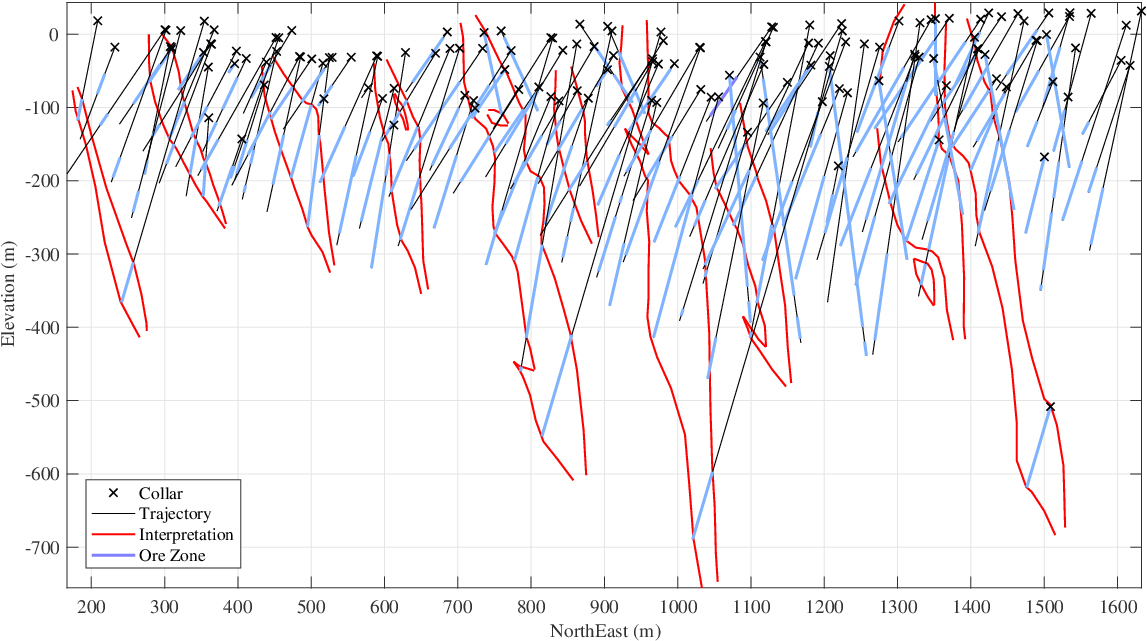
\includegraphics[width=0.8\textwidth]{capitulo_2/secoes.jpg}\label{a}}\\
\end{center}
\begin{center}
\subfloat[][Modelo implícito.]{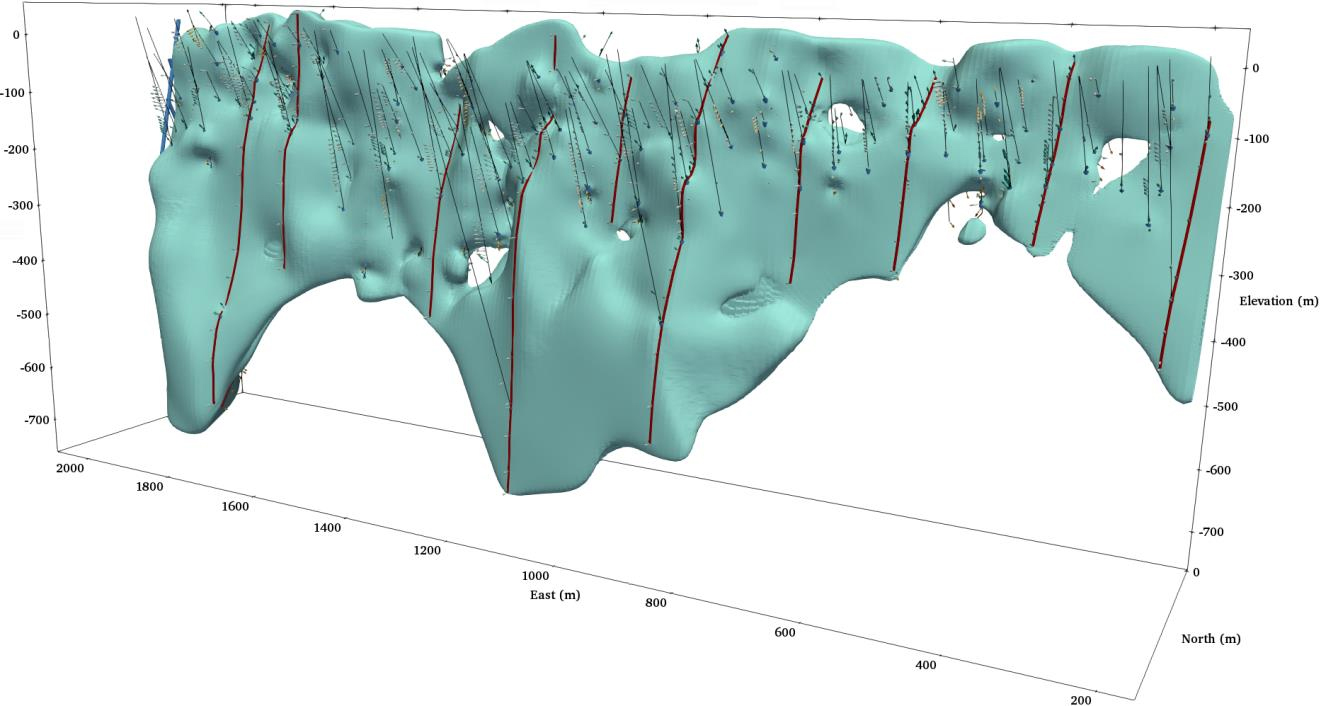
\includegraphics[width=0.8\textwidth]{capitulo_2/modelo_mls.jpg}\label{b}}
\legend{Fonte: \citeonline{manchuck_MLS}}
\end{center}
\end{figure}

A incerteza pode ser avaliada pelo método por meio do parâmetro de incerteza C e simulações não condicionais. 

Apesar da integração furos/interpretação ser muito promissora já que são duas fontes de dados que serão utilizadas na geração do modelo. O método é recente e ainda apresenta alguns desafios operacionais, principalmente em relação à exigência de estruturas planares e avaliação de incerteza.

\section{Avaliação da incerteza}

Sempre existirá algum grau de incerteza nos volumes geológicos modelados, que varia de acordo com o número de amostras e a informação geológica disponível. A incerteza do modelo geológico, muitas vezes, pode ser a maior fonte de incerteza do projeto mineiro. Por esse motivo, diversos métodos foram desenvolvidos com o objetivo de avaliar a incerteza dos modelos geológicos a partir das funções distância assinaladas.

Essa seção abordará os métodos disponíveis na literatura com exemplos práticos no banco de dados apresentado.

\subsection{Avaliação heurística da incerteza}\label{heuristic}

O método mais simples de avaliação de incerteza em modelos geológicos implícitos, proposto por \citeonline{silvaanddeutschccgmodeling}, consiste em transformar distâncias estimadas em probabilidades via \textit{softmax transformation}. Técnica amplamente usada em métodos de classificação para múltiplas classes \cite{mccullaghgeneralizedlinear}. A ideia é transformar as distâncias estimadas em probabilidades a partir da \autoref{eq_softmax}. Os valores transformados encontram-se entre zero e um e  sua soma deve ser igual a um, para cada bloco estimado.

\begin{equation}
	P(i(u)=k)=\frac{e^\frac{-d^*_k(u)}{\gamma}}{\sum_{k'=1}^{K}e^\frac{-d^*_k(u)}{\gamma}}
    \label{eq_softmax}
\end{equation}

$P(i(u)=k)$ representa a probabilidade de um local $u$ pertencer à categoria $k$, $d^*_k(u)$ é a distância estimada para a categoria $k$ e $\gamma$ é um parâmetro que regula a inter-relação entre as probabilidades das $K$ diferentes categorias. Quanto maior $\gamma$, maior as diferenças entre as probabilidades (maior a banda de incerteza), como pode ser observado na \autoref{softmax_ex}. \citeonline{silvaanddeutschccgcorrecting} advogam que o parâmetro pode ser a maior distância estimada entre todas as categorias.

Para exemplificar a transformação, a \autoref{softmax_grafico}, mostra à esquerda as distâncias estimadas para cada uma de cinco categorias em um mesmo bloco em particular. À direita as distâncias transformadas pela \autoref{eq_softmax} em probabilidades daquele bloco pertencer a cada uma das cinco categorias. Observe que distâncias menores (mais negativas) geram probabilidades maiores, e vice-versa.  

\begin{figure}[H]
	\caption{\label{softmax_grafico}Distâncias estimadas e transformadas em probabilidades para um mesmo bloco.}
	\begin{center}
		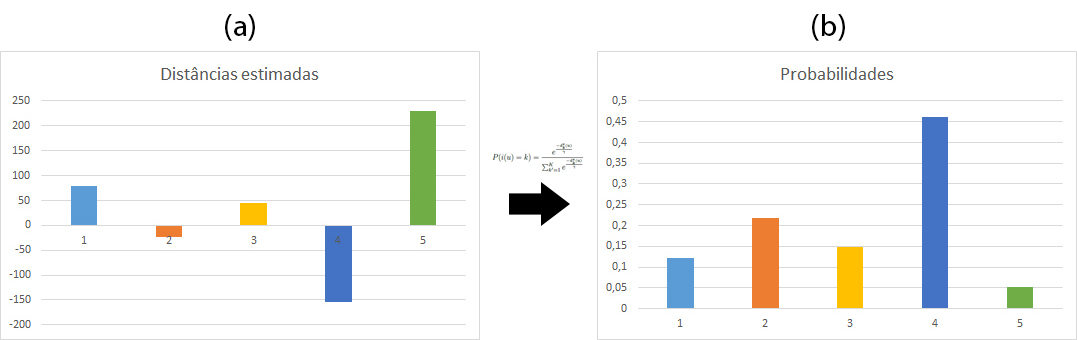
\includegraphics[width=0.7\textwidth]{capitulo_2/softmax_bars_final.jpg}
	\end{center}
	\legend{Fonte: \citeonline{rolo_dissertacao}}
\end{figure}

A \autoref{softmax_ex} mostra seções em XZ do mapa de probabilidades para a categoria 1, com diferentes valores para $\gamma$.

\begin{figure}[H]
\caption{Seções em XZ do mapa de probabilidades para a categoria 1 com diferentes valores para $\gamma$.} 
\label{softmax_ex}
\begin{center}
\subfloat[][$\gamma=30$]{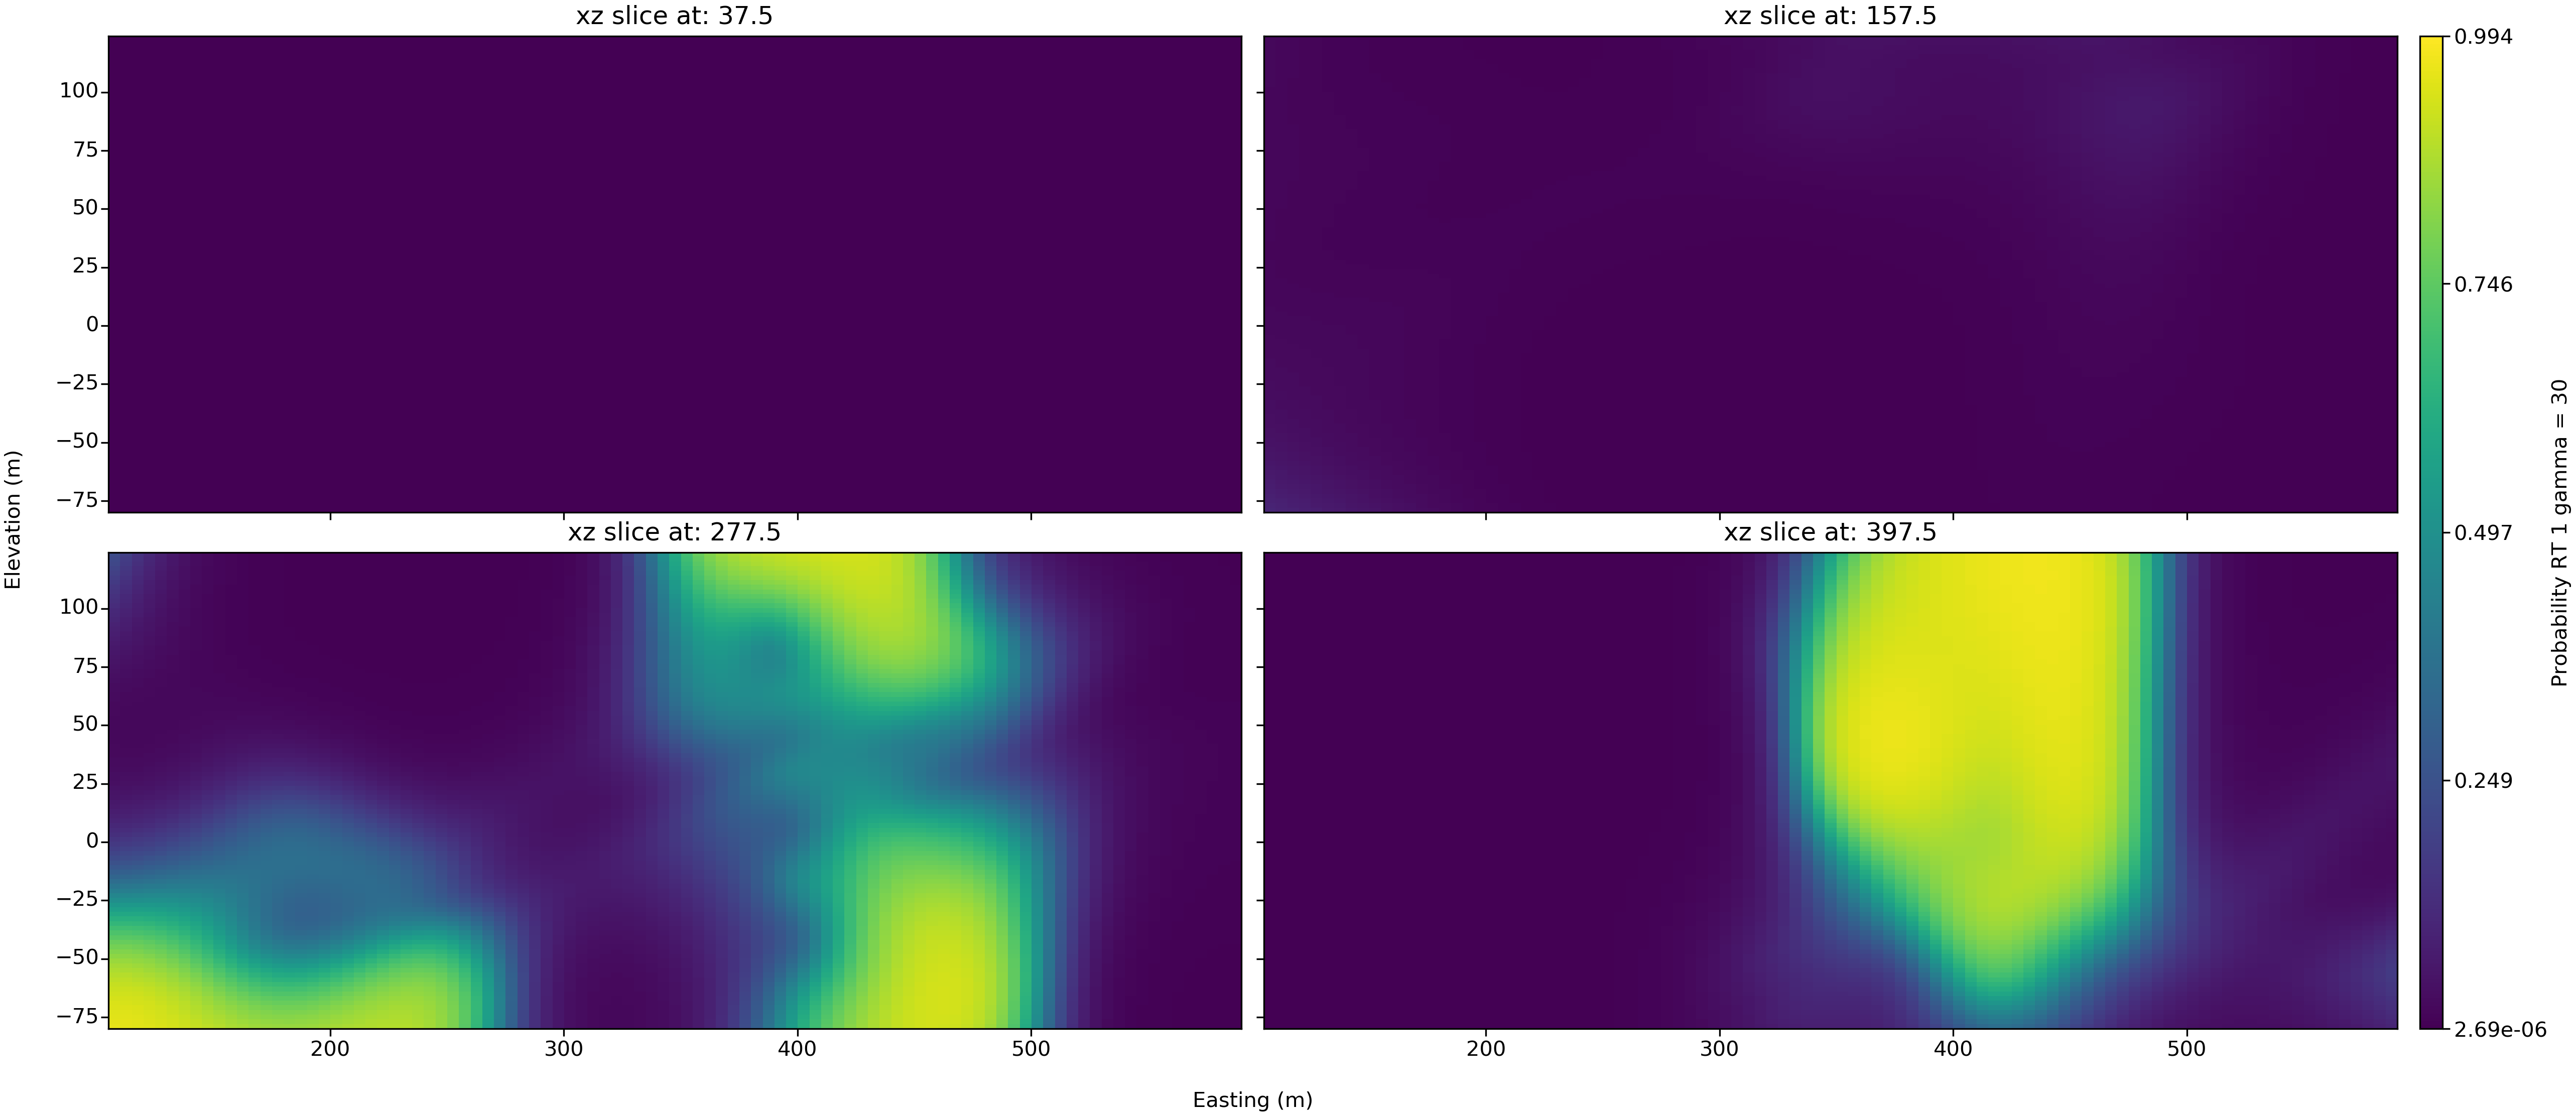
\includegraphics[width=0.8\textwidth]{capitulo_2/xz_30.png}\label{a}}\\
\end{center}
\begin{center}
\subfloat[][$\gamma=50$]{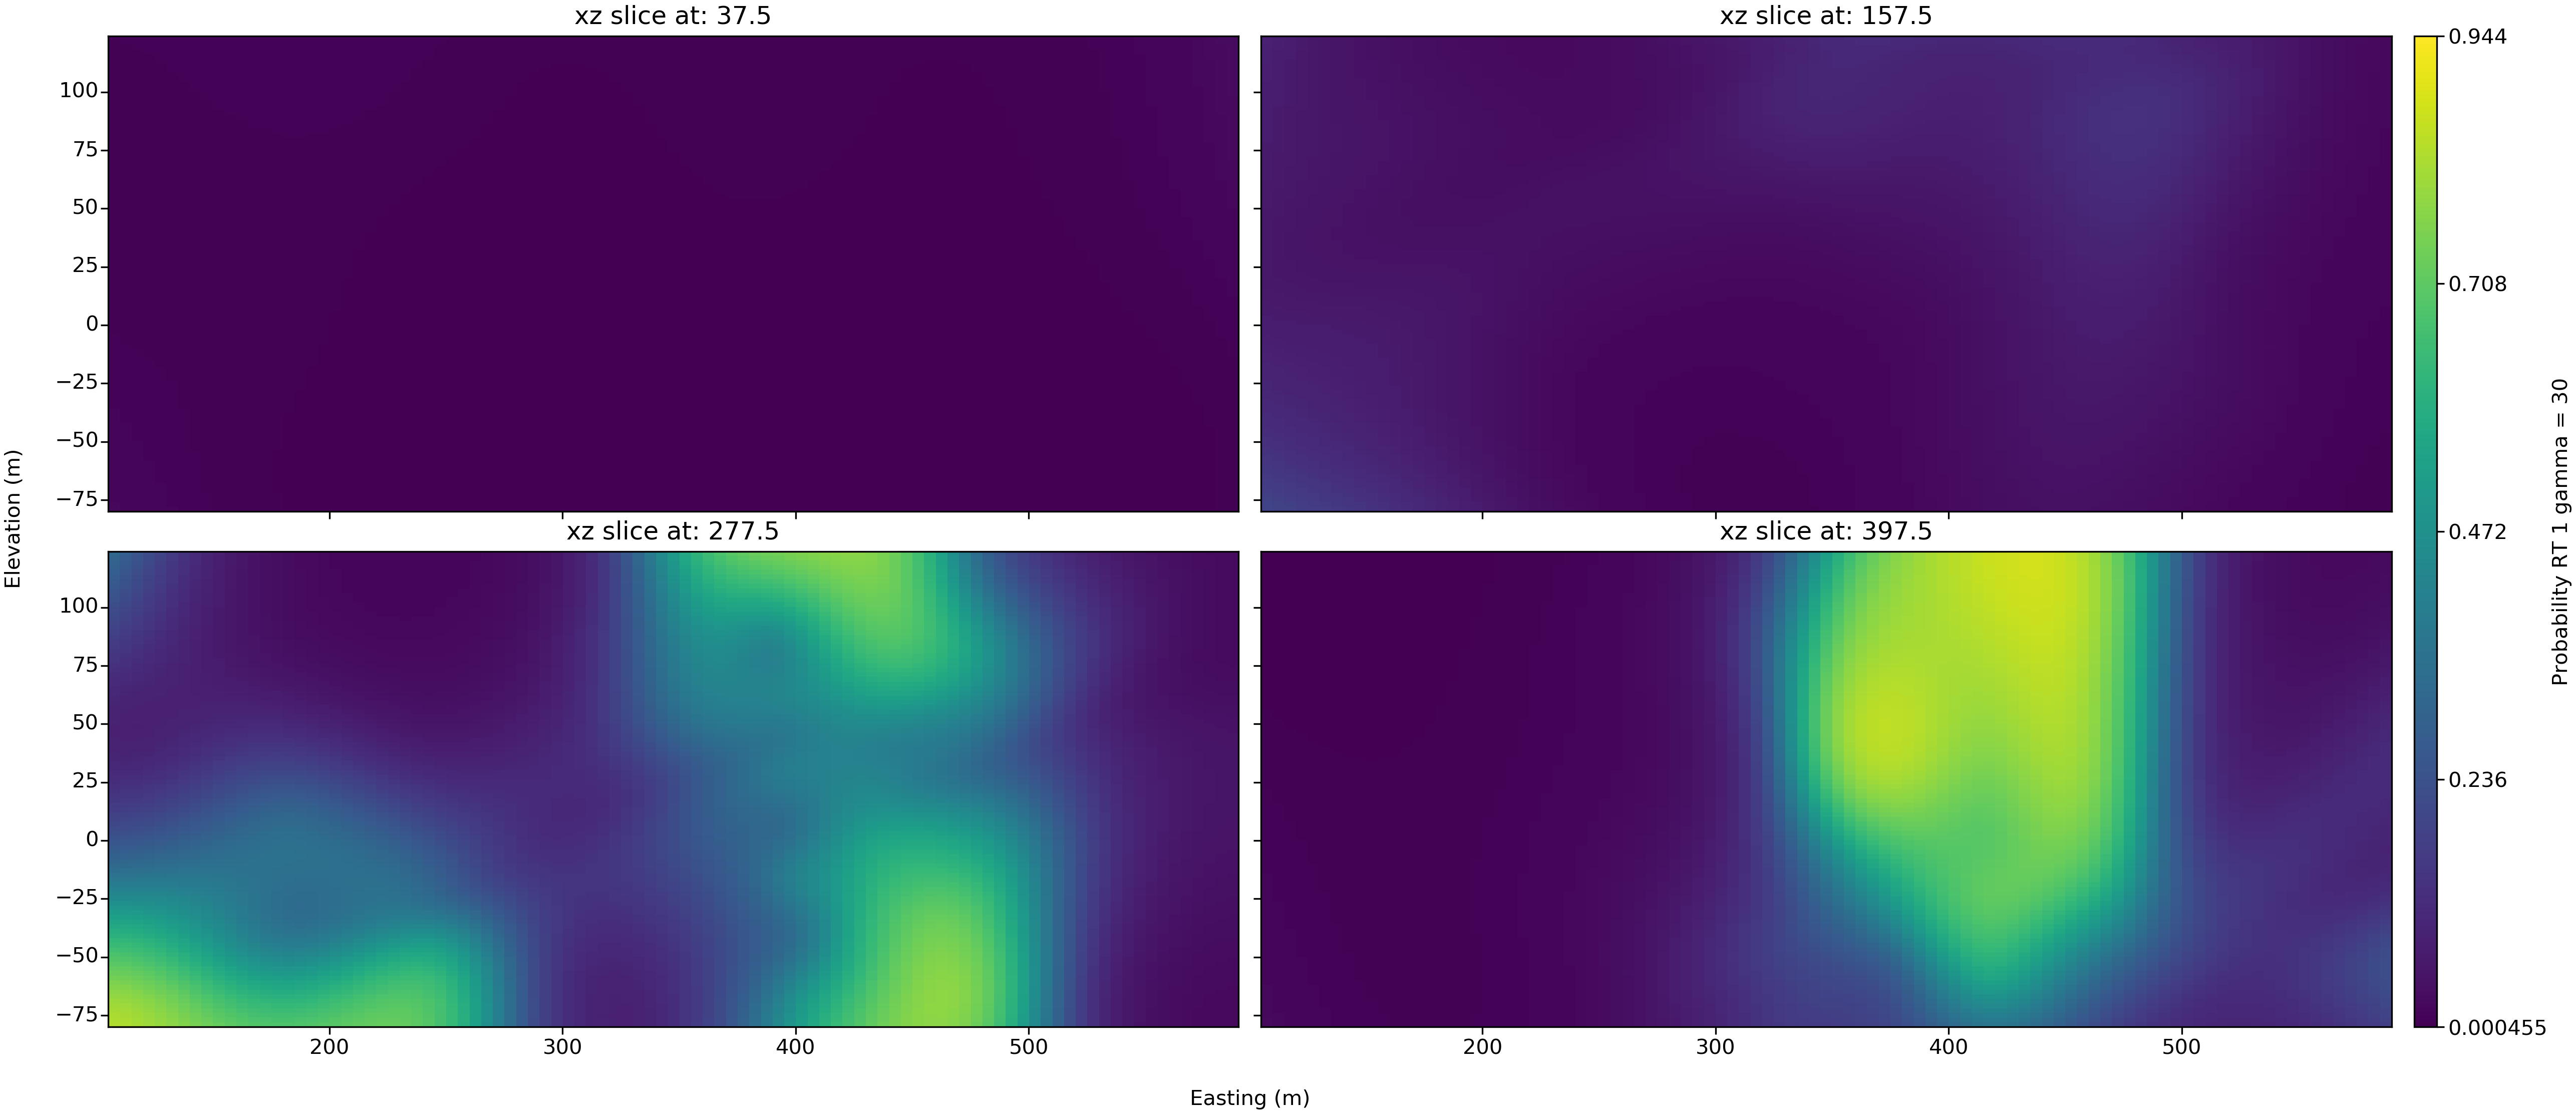
\includegraphics[width=0.8\textwidth]{capitulo_2/xz_50.png}\label{b}}
\end{center}
\end{figure}

Apesar do método ser simples e direto, suportar múltiplas categorias simultaneamente, seu resultado não pode ser utilizado em etapas subsequentes do processo de  avaliação, por não gerar múltiplas realizações do modelo geológico. Além disso, A escolha do parâmetro $\gamma$ é subjetiva e dependa da distribuição espacial das amostras, dependendo da escolha para o parâmetro nem mesmo blocos colocados com amostras recebem a probabilidade 100\%. 

\subsection{\textit{Boundsim}}

Uma outra metodologia proposta por \citeonline{mclennan2006boundsim} consiste em realizar um \textit{bootstrap} espacial \cite{deutsh_spatial_bootstrap} da média da distância assinada calculada para uma dada categoria. O procedimento de \textit{bootstrap} é amplamente utilizado para quantificar incerteza em parâmetros estatísticos, As duas mais importantes suposições são: os dados são representativos e os dados são independentes. Por esse motivo, a técnica de amostragem deve ser modificada para variáveis que apresentam continuidade espacial. A \autoref{bs_df_1} mostra o histograma da média para as distâncias assinaladas da categoria 1 do banco de dados. 

\begin{figure}[H]
	\caption{\label{bs_df_1}Histograma do bootstrap espacial da média das distâncias assinaladas para a categoria 1.}
	\begin{center}
		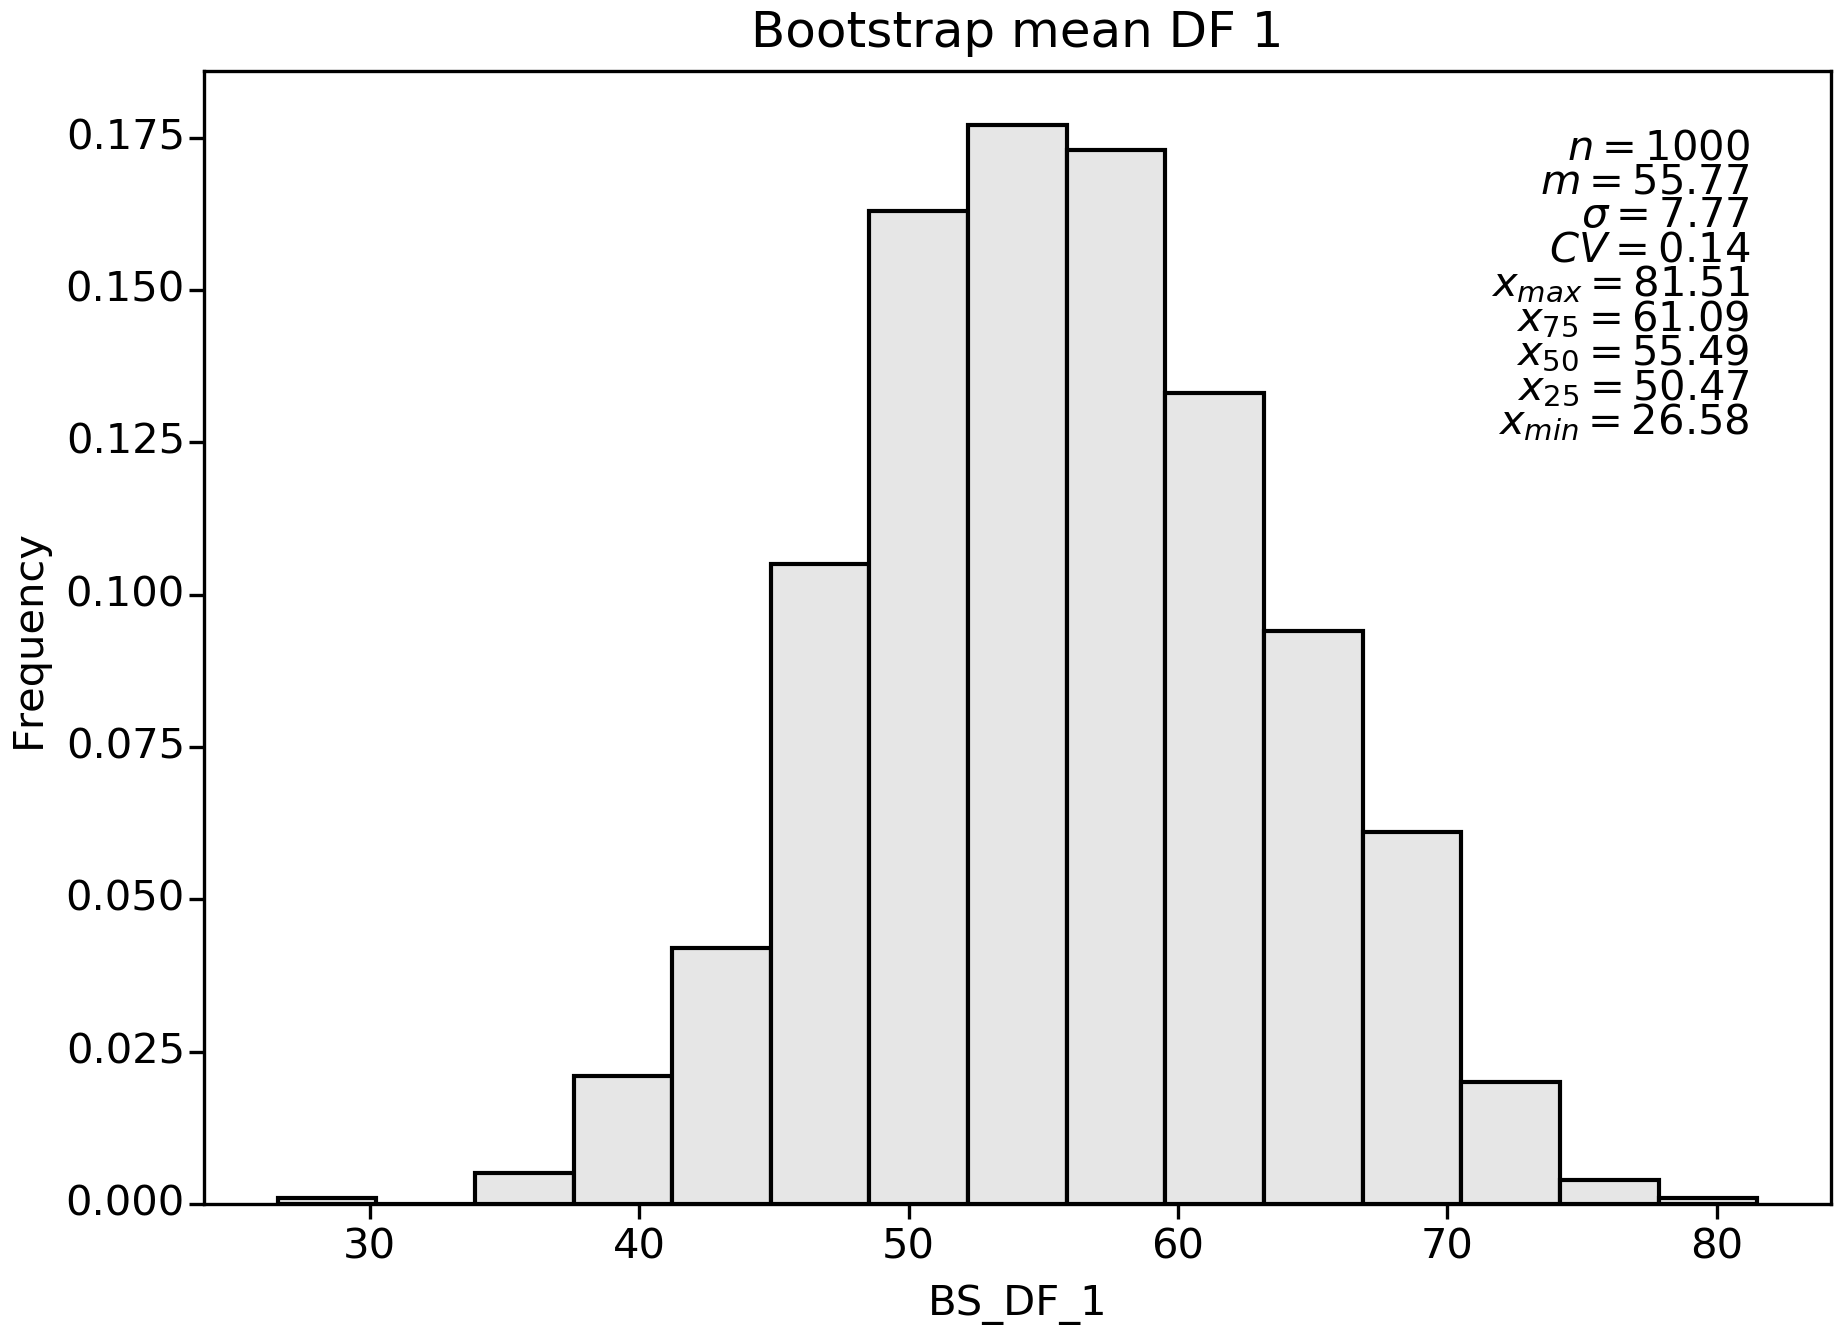
\includegraphics[width=0.5\textwidth]{capitulo_2/BS_DF_1.png}
	\end{center}
	%\legend{Fonte: \citeonline{rolo_dissertacao}}
\end{figure}

Valores para a média são tomados do histograma da média, gerado pelo \textit{bootstrap} espacial. Esses valores podem ser correspondentes ao p10, p50 e p90 por exemplo.

Então, as distâncias assinaladas são interpolados para os nós do grid por krigagem simples, que tem como hipótese a estacionariedade da média por todo o domínio. A média estacionária para a krigagem simples são os valores tomados do histograma.

O último passo consiste em extrair a iso superfície zero dos modelos implícitos gerados por krigagem simples com os diferentes valores da média estacionária tomadas do histograma da média. Em tese, quanto maior o percentil menor o risco associado, o volume do sólido modelado infla ou contrai de acordo com o valor escolhido para a média estacionária.

A \autoref{boundsim_table} mostra os blocos classificados como pertencentes à categoria 1 usando a metodologia apresentada, com valores de média estacionária correspondentes à p10, p50 e p90.

\begin{table}[H]
\begin{center}
\begin{tabular}{lr}
Percentil & \multicolumn{1}{l}{Blocos dentro} \\ \hline
10 & 109886 \\
50 & 110446 \\
90 & 111069 \\ \hline
\end{tabular}
\end{center}
\caption{Blocos classificados como pertencentes à categoria 1.}\label{boundsim_table}
\end{table}

A metodologia é simples e direta, porém, deve ser aplicada à uma categoria por vez, na presença de múltiplos domínios alguma abordagem hierárquica deve ser estabelecida. A sensibilidade da krigagem simples à média depende da configuração espacial das amostras, muitas vezes a diferença entre os volumes obtidos é irrelevante, como no caso do banco de dados em estudo: a diferença no volume do sólido do caso mais conservador para o de maior risco é de pouco mais de 1\%. As iso superfícies são praticamente coincidentes.

O produto final do método pode ser utilizado nas etapas subsequentes do processo de avaliação, todavia, o método não avalia incerteza de forma adequada. Os autores do estudo original aplicaram a metodologia apenas em bancos de dados sintéticos e de geometria regular. 

\subsection{Simulação direta das distâncias assinaladas}\label{sim_direta}

\citeonline{caceres2011stochastic} e \cite{radtke_dissertacao} propuseram que as distâncias assinaladas sejam simuladas de forma direta: a partir de um modelo geológico implícito multi categórico (\autoref{multi_cat}) um coeficiente U de incerteza deve ser calculado de acordo com \autoref{u_eq}:

\begin{equation}\label{u_eq}
    U(u)=\frac{max\{D_{min}\}-min\{d^*_k(u)\}^K_{k=1}}{max\{D_{min}\}-min\{D_{min}\}}
\end{equation}

Onde:

\begin{equation}
    D_{min}=\{min\{d^*_k(u_1)\},...,\{min\{d^*_k(u_n)\}^K_{k=1}\}
\end{equation}

E $d^*_k(u)$ é a distância estimada no local u para a categoria k.

Os valores de U variam entre 0 e 1, um \textit{cutoff} em U determina a extensão da zona de incerteza ao redor dos contatos: quanto mais próximo de 1, mais estreita a zona. A \autoref{u_fig} mostra o coeficiente U calculado para todos os nós do grid a partir do modelo da \autoref{multi_cat_rbf}.

\begin{figure}[H]
	\caption{\label{u_fig}Coeficiente U calculado para todos os nós do grid.}
	\begin{center}
		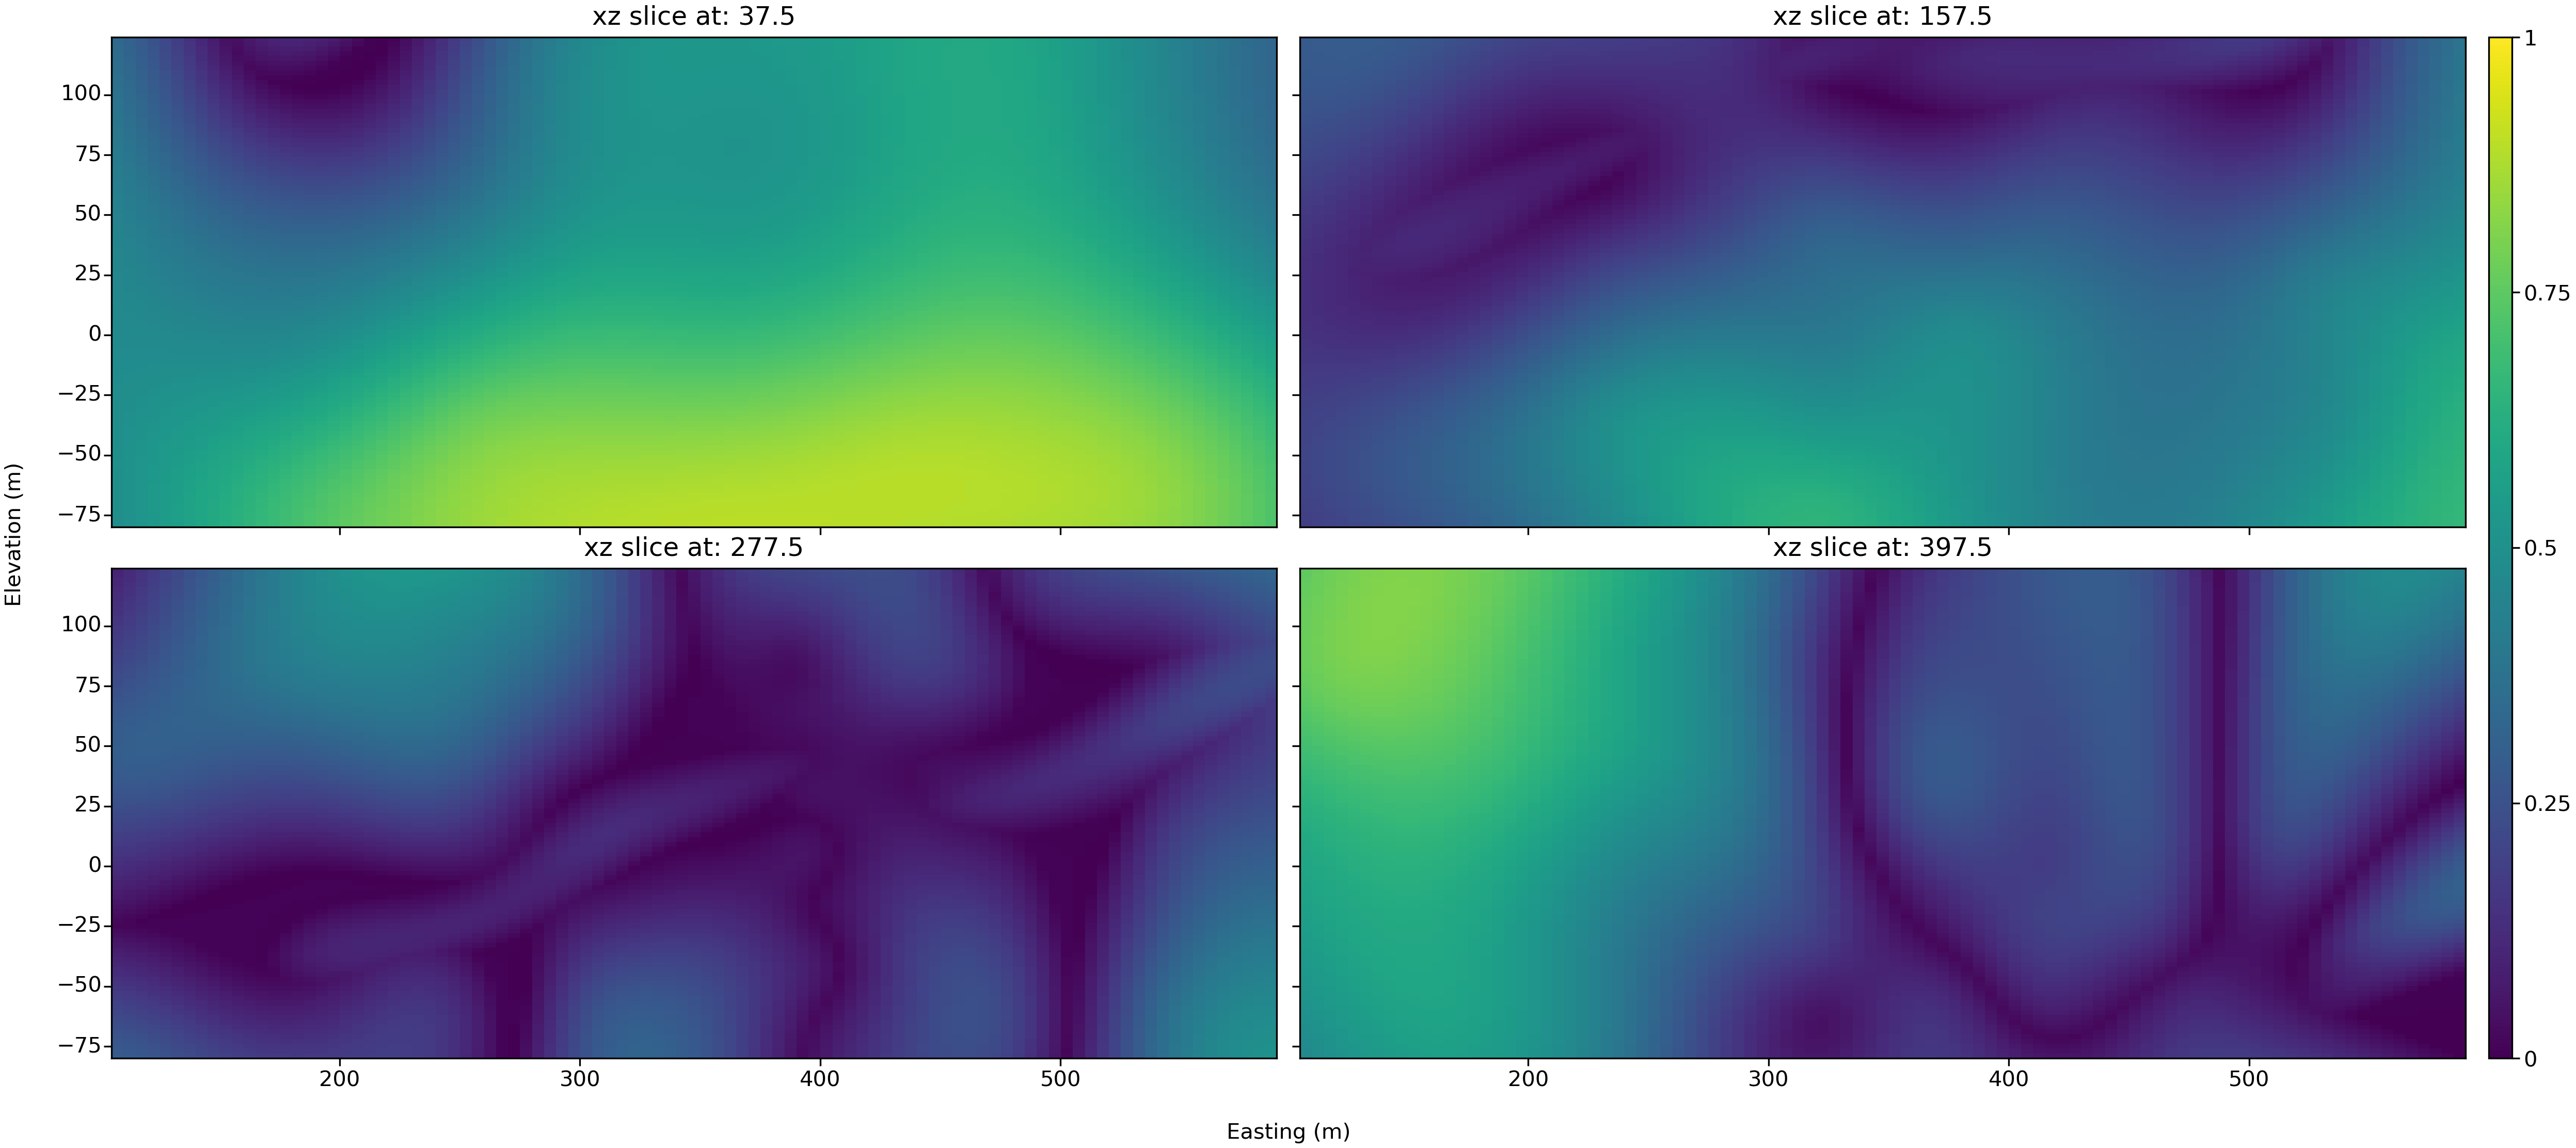
\includegraphics[width=0.8\textwidth]{capitulo_2/u_coef.png}
	\end{center}
	%\legend{Fonte: \citeonline{rolo_dissertacao}}
\end{figure}

Um \textit{cutoff} em 0.8 foi aplicado em U e as distâncias assinaladas foram simuladas por simulação sequencial Gaussiana na região de incerteza. A \autoref{dist_sim_u} mostra as distâncias simuladas para as três categorias do banco de dados na zona de incerteza. 

\begin{figure}[H] 
    \caption{Distâncias simuladas na zona de incerteza para as categorias do banco de dados.} \label{dist_sim_u}
     \centering
     \subfloat[][Categoria 1]{\includegraphics[width=.3\textwidth]{capitulo_2/Ucutoff1.png}\label{<figure1>}}
     \subfloat[][Categoria 2]{\includegraphics[width=.3\textwidth]{capitulo_2/Ucutoff2.png}\label{<figure2>}}
     \subfloat[][Categoria 3]{\includegraphics[width=.3\textwidth]{capitulo_2/ucutoff3.png}\label{<figure2>}}
\end{figure}

A categoria correspondente ao menor valor simulado é retida em cada bloco e os blocos simulados são concatenados com os blocos estáticos, atribuídos pela interpolação.

A \autoref{dif_real} mostra duas diferentes realizações do modelo geológico estocástico criado a partir da simulação direta das distâncias.

\begin{figure}[H]
\caption{Diferentes realizações do modelo geológico.} 
\label{dif_real}
\begin{center}
\subfloat[][Realização 1]{\includegraphics[width=0.8\textwidth]{capitulo_2/directsimreal1.png}\label{a}}\\
\end{center}
\begin{center}
\subfloat[][Realização 2]{\includegraphics[width=0.8\textwidth]{capitulo_2/directsimreal2.png}\label{b}}
\end{center}
\end{figure}

O método é baseado em múltiplas realizações do modelo geológico, então, seu produto final pode ser usado nas etapas posteriores do processo de avaliação. Entretanto, a metodologia tem muitos passos \cite{radtke_dissertacao}

\begin{enumerate}
\item Cálculo das distâncias assinaladas para todas as amostras e categorias;
\item Variografia das distâncias no espaço original para todas as categorias;
\item Interpolação das distancias; 
\item criação do modelo com base na menor distância interpolada;
\item Criação da zona de incerteza;
\item Transformação Gaussiana das distâncias;
\item Variografia das distâncias no espaço gaussiano para todas as categorias;
\item Geração de múltiplos modelos baseados na menor distância simulada;
\item Validação e pós processamento das realizações.
\end{enumerate}

Além disso, a simulação é muito sensível aos parâmetros, o que muitas vezes, gera modelos com muito ruído, que não são geologicamente realistas, e não honram as amostras, como os da \autoref{dif_real}. O resultado final não justifica o número excessivo de passos e parâmetros. O coeficiente U não controla a magnitude da incerteza, apenas diminui o tempo das simulações, o magnitude da incerteza é controlada pelo parâmetros da simulação.

\subsection{Simulação multi ponto}

\citeonline{silvaenhancedgeomodeling} propôs uma metodologia que integra modelagem geológica implícita com funções distâncias assinaladas e simulação geostatística multi ponto. A geostatística multi ponto utiliza imagens de treinamento para extrair e reproduzir estruturas geológicas complexas. Geralemnte, imagens de trinamento são baseadas em modelos conceituais do fenômeno geoógico. Em seu trabalho, \citeonline{silvaenhancedgeomodeling} cria imagens de trinamento a partir de modelos geológicos implícitos determinísticos criados com funções distância assinaladas e modelos estocásticos criados por simulação sequencial dos indicadores. No trabalho é introduzida uma metodologia  para integrar múltiplas imagens de treinamento, uma metodologia para calibrar a contribuição de cada imagem de treinamento e uma medida de entropia multi ponto ao longo dos furos de sondagem.

\citeonline{silvaenhancedgeomodeling} concluiu que imagens de treinamento geradas a partir das amostras produzem modelos geológicos estocásticos por MPS melhores. A \autoref{snesim_real} mostra duas realizações do modelo geológico criado a partir da aplicação do algoritmo \verb|snesim| usando a \autoref{multi_cat_rbf} como imagem de treinamento. 

\begin{figure}[H]
\caption{Diferentes realizações do modelo geológico.} 
\label{snesim_real}
\begin{center}
\subfloat[][Realização 1]{\includegraphics[width=0.8\textwidth]{capitulo_2/snesim_real1.png}\label{a}}\\
\end{center}
\begin{center}
\subfloat[][Realização 2]{\includegraphics[width=0.8\textwidth]{capitulo_2/snesim_real2.png}\label{b}}
\end{center}
\end{figure}

Os modelos mostram realismo geológico, não apresentam ruido excessivo. Além disso, o método é rápido e não depende de um grande número de parâmetros. Em contrapartida, não é possível controlar a magnitude da incerteza. 

\subsection{\textit{Boundary simulation}}\label{boundsim}

A metodologia proposta por \citeonline{wilde_sim_bound_reals} consiste em gerar realizações das fronteiras geológicas comparando distâncias modificadas interpoladas com simulações não condicionais. 

O primeiro passo é calibrar os parâmetros de incerteza, \citeonline{munroe_c_full_calibration} propuseram a calibração completa dos parâmetros C e $\beta$, onde C controla a largura da bande de incerteza e $\beta$ controla o viés. Os parâmetros devem ser otimizados para que a incerteza apropriada seja avaliada. Otimizar esses parâmetros é uma operação computacionalmente cara que requer múltiplos modelos de referência e duas funções objetivo \cite{wilde2012kriging}.

\citeonline{kaperov_review_boundary} propuseram uma metodologia de calibração para o parâmetro C simplificada, de modo empírico. considerando a malha amostral e a experiência e conhecimento do geomodelador.

\citeonline{wilde_new_way} propuseram uma outra metodologia de calibração, nessa metodologia apenas o parâmetro C é calibrado usando apenas as amostras disponíveis. Um subconjunto das amostras é removido antes do cálculo das distâncias assinaladas. Isso cria dois diferentes bancos dados: o banco de dados das distâncias assinaladas e o banco de dados \textit{jackknife}. O banco de dados das distâncias assinaladas é usado para condicionar a estimativa das distâncias nos locais do banco de dados \textit{jackknife}. Algumas amostras do banco de dados \textit{jackknife} que foram codificadas como fora do domínio terão distâncias estimadas negativas (dentro do domínio) e vice-versa. O parâmetro C é ajustado até que uma proporção pré definida de classificação errônea seja atingida.

A \autoref{c_param_1} mostra a calibração do parâmetro C para a categoria 1 do banco de dados. 25\% das amostras foram removidas de forma aleatória 50 vezes, gerando 50 bancos de dados de distância e 50 bancos de dados \textit{jackknife}, as distâncias foram estimados nos locais das amostras \textit{jackknife} e a taxa de classificação errônea foi registrada no eixo y. o parâmetro C foi incrementado, e somado ou subtraídos das distâncias de acordo com a \autoref{C_dist}, o processo é repetido enquanto C varia de 0 até 250m. Quanto maior for o valor de C, menor o índice de classificação errônea.

\begin{figure}[H]
	\caption{\label{c_param_1}Calibração do parâmetro C para a categoria 1.}
	\begin{center}
		\includegraphics[width=0.6\textwidth]{capitulo_2/uncert_1.png}
	\end{center}
	%\legend{Fonte: \citeonline{rolo_dissertacao}}
\end{figure}

\begin{equation}
	d_k(u_\alpha)=\begin{cases}
	-\parallel u_\alpha-u_\beta\parallel - C,\:\textrm{se $u_\alpha$ pertence ao domínio}\\
	+\parallel u_\alpha-u_\beta\parallel + C,\:\textrm{se $u_\alpha$ não pertence ao domínio}\end{cases}
    \label{C_dist}
\end{equation}

O valor do parâmetro C deve ser determinado a partir da calibração (\autoref{c_param_1}). \citeonline{manchuck_deutsch_Geometric} sugerem 2,5\% de classificação errônea em nível aceitável para depósitos tabulares, uma outra forma de escolha é o método do cotovelo, o valor tomado deve ser o ponto de inflexão da curva. Para a categoria 1 foi tomado o valor de C igual a 130 que corresponde a um índice de classificação errônea de 2\%. As distâncias modificadas pelo parâmetro C a partir da \autoref{C_dist} devem ser interpoladas para todos os nós do grid, e a truncagem entre -C e C define a zona de incerteza.

Valores para a função distância são então simulados uniformemente entre -C e C. Caso o valor interpolado seja menor que o valor simulado para a função distância, o local é considerado pertencente ao domínio, caso o valor seja maior, o local é considerado externo ao domínio. Nos locais onde a interpolação apresenta o mesmo valor da simulação são estabelecidos os contatos dos domínios como esquematizado na \autoref{class}.

\begin{figure}[H]
	\caption{\label{class}Classificação dos locais comparando valores estimados e simulados.}
	\begin{center}
		\includegraphics[width=0.8\textwidth]{capitulo_2/classificacao.png}
	\end{center}
	\legend{Fonte: Modificado de \citeonline{wilde_sim_bound_reals}}
\end{figure}

Para que a simulação seja realizada de forma uniforme entre –C e +C, o desvio padrão $y`(u)$, deve ser simulado e transformado pela relação:

\begin{equation}
    df'(u)=2*C*G^-1(y'(u))-C
\end{equation}

Onde: $df'(u)$ é o valor da função distância simulada, $y'(u)$ o valor normal padrão da simulação não condicional, e $G^-1$ representa a determinação do valor da distribuição acumulada padrão normal correspondente a $y'(u)$. Para garantir que os valores pertençam a região estabelecida. os valores são multiplicados por 2C e subtraídos de C.

O variograma utilizado na simulação não condicional pode ser o mesmo das distâncias assinaladas. O alcance do variograma determina a natureza do contato entre os domínios, menores alcances geram contatos mais rugosos enquanto maiores alcances, contatos suaves.

A \autoref{cat1_bound_sim} mostra as distâncias interpoladas e simuladas na zona de incerteza para a a categoria 1, definida entre -120m e 120m e os blocos classificados em pertencentes à categoria ou não. As probabilidades de cada bloco pertencer à categoria 1 pode ser calculada tomando a média dos blocos classificados com 1 ou 0 em todas as realizações.

\begin{figure}[H] 
    \caption{Interpolação, simulação e classificação na zona de incerteza.} \label{cat1_bound_sim}
     \centering
     \subfloat[][Distâncias interpoladas]{\includegraphics[width=.3\textwidth]{capitulo_2/interpolated.jpeg}\label{<figure1>}}
     \subfloat[][Distâncias simuladas]{\includegraphics[width=.3\textwidth]{capitulo_2/simulated.jpeg}\label{<figure2>}}
     \subfloat[][Classificação]{\includegraphics[width=.3\textwidth]{capitulo_2/classification.jpeg}\label{<figure2>}}
\end{figure}

A \autoref{cpar_real} mostra seções em XY e YZ de uma das realizações para a categoria 1.

\begin{figure}[H]
\caption{Seções verticais de uma realização para a categoria 1.} 
\label{cpar_real}
\begin{center}
\subfloat[][Seção em XY]{\includegraphics[width=0.8\textwidth]{capitulo_2/cpar1.png}\label{a}}\\
\end{center}
\begin{center}
\subfloat[][Seção em YZ]{\includegraphics[width=0.8\textwidth]{capitulo_2/cparyz.png}\label{b}}
\end{center}
\end{figure}

O método é rápido já que é baseado em simulações não condicionais, gera modelos realistas sem ruído e com fronteiras contínuas. Tanto a magnitude da incerteza quanto a natureza da fronteira podem ser controlados. Entretanto, o método funciona apenas para uma categoria por vez e mesmo que simplificações tenham sido desenvolvidas, a calibração do parâmetro de incerteza ainda pode ser laboriosa e subjetiva.

\citeonline{amarante_incerteza_associada} propuseram uma adaptação  do método para múltiplas categorias simultâneas, uma série de regras hierárquicas baseadas na cronologia dos eventos geológicos devem ser definidas, a \autoref{hier_ex} mostra um esquema do método, evidenciando as regras de hierarquização e realizações dos grupos formados. Embora seja uma alternativa para ambientes multi categóricos, a definição das regras de hierarquização dependem de conhecimento geológico além das amostras, e muitas vezes indisponível.

\begin{figure}[H]
	\caption{\label{hier_ex}Esquema do método mostrando as regras de hierarquização e diferentes realizações dos grupos formados.}
	\begin{center}
		\includegraphics[width=0.9\textwidth]{capitulo_2/hier_example.png}
	\end{center}
	\legend{Fonte: \citeonline{amarante_incerteza_associada}}
\end{figure}

\subsection{Sumário dos métodos de avaliação de incerteza}

A \autoref{sumario} mostra um sumário dos métodos de incerteza que avalia: a simplicidade, o método deve, preferencialmente, ser simples e direto, não deve envolver um número excessivo de passos ou matemática complicada. A velocidade, o método deve ser de rápida execução. A capacidade de trabalhar em ambientes multi categóricos de forma direta, sem a necessidade de abordagens hierárquicas subjetivas. O realismo geológico, as formas geradas devem ser suaves e não apresentar ruído excessivo. O controle da incerteza, a incerteza deve ser controlada a partir de bandas de incerteza ou a partir dos parâmetros de simulação. Finalmente, a natureza do contato, ruidoso ou suave, deve ser controlada.

% Table generated by Excel2LaTeX from sheet 'Planilha1'
\begin{table}[H]
  \centering
  \resizebox{\textwidth}{!}{%
    \begin{tabular}{lcccccc}
    Método & \multicolumn{1}{l}{Simplicidade} & \multicolumn{1}{l}{Velocidade} & \multicolumn{1}{l}{Multi categórico} & \multicolumn{1}{l}{Realismo geológico} & \multicolumn{1}{l}{Controle da incerteza} & \multicolumn{1}{l}{Controle do tipo de contato} \\
    \midrule
    Heurístico & simples & rápido & sim   & não   & sim   & não \\
    Boundsim & simples & rápido & não   & sim   & não   & não \\
    Simulação direta & complexo & demorado & sim   & não   & sim   & não \\
    MPS   & simples & rápido & sim   & sim   & não   & não \\
    Boundary simulation & simples  & rápido & não   & sim   & sim   & sim \\
    \bottomrule
    \end{tabular}%
    }
  \caption{Sumário dos métodos de avaliação de incerteza de modelos geológicos.}\label{sumario}%
\end{table}%





\chapter{Proposta de tese}

\section{Problemas e relevância da tese}\label{problemas}

A modelagem geológica implícita com funções distância assinaladas é uma metodologia bem estabelecida que permite ao gemodelador gerar de forma rápida modelos geológicos reprodutíveis, consistentes e checáveis a partir de uma função volume derivada a partir dos dados amostrais. 

Porém, existem alguns pontos problemáticos e limitantes na metodologia que merecem atenção. A não estacionariedade da função distância assinalada torna a modelagem dos variogramas arbitrária e questionável.

Apesar dos métodos implícitos serem totalmente independentes de um \textit{grid}, o objetivo final da modelagem geológica implícita é preencher o \textit{grid} de estimativas com as litologias correspondentes. Para um número constante de amostras, o tempo requerido para interpolar a função volume para todos os nós do \textit{grid} aumenta linearmente em relação ao número de nós. Os parâmetros do \textit{grid} de estimativa podem ser pré-determinados pelos parâmetros de engenharia do projeto, porém, o \textit{grid} de definição do modelo geológico não necessariamente deve ser o mesmo do \textit{grid} de estimativa. A consideração mais importante na definição do \textit{grid} é que a resolução seja suficiente para captar as estruturas geológicas de interesse \cite{martin2017implicitmodeling}. É preciso encontrar um balanço entre número de nós e resolução necessária. A resolução do \textit{grid} influencia diretamente a avaliação de incertezas.

A função volume, i.e. função distância assinalada, calculada em cada ponto amostral é interpolada. Diferentes métodos podem ser usados, desde métodos que não apresentam muita complexidade como os do inverso da distância, quanto métodos mais complexo como krigagem global ou funções de bases radiais com anisotropia global ou local. A escolha do interpolador muitas vezes é subjetiva e confusa e depende dos objetivos e da complexidade da geologia do depósito. Exitem problemas relacionados à estacionariedade quando a krigagem é o método utilizado. A estratégia de busca é ponto crítico para nos interpoladores não globais.

Na presença de múltiplos domínios, principalmente em ambientes geológicos complexos, é necessário a aplicação de uma lógica de precedência de estruturas ao invés de simplesmente tomar a menor distância assinalada para a criação de modelos realistas. Mesmo em ambientes sem complexidade, categorias com poucas amostras disponíveis muitas vezes desaparecem dos modelos gerados tomando a menor distância estimada (se não for usada uma sequência hierárquica.).

Alguns dos métodos de avaliação de incerteza, encontrados na literatura, exigem a calibração de uma zona de incerteza entre diferentes domínios geológicos. Enquanto para alguns métodos, a definição da zona é subjetiva e não segue nenhuma regra matemática ou geológica, em outros a definição da zona de incerteza é extremamente laboriosa e complicada.
Existem diferentes métodos para avaliação de incerteza em modelos geológicos implícitos. Em alguns deles, é possível avaliar a incerteza de todas as diferentes litologias do depósito mineral simultaneamente, em outros a incerteza associada à cada litologia deve ser avaliada separadamente. Além disso, a magnitude da incerteza e a natureza dos contatos não podem ser controladas na maior parte dos métodos encontrados na literatura.

Estruturas geológicas específicas, como lentes ou diques, podem desaparecer, ou não serem bem reproduzidas nos modelos implícitos, principalmente, quando sub-amostradas em relação às demais estruturas. Além disso, a metodologia, por si só, não produz bons resultados ao tentar reproduzir falhas e dobras. 

Segundo o estatístico \citeonline{box1979robustness}: \textit{"Todos os modelos estão errados, mas alguns são úteis."} A modelagem implícita é conhecida por criar modelos de forma rápida e simples, porém, modelos ruins de forma rápida e simples. É necessário checar se os modelos implícitos honram a geologia do depósito e serão úteis para o processo de avaliação de recursos/reservas. 

Essa tese encontra relevância ao buscar solução para os problemas abordados e propor melhorias para a técnica, que vem sendo aplicada com sucesso na indústria mineral há mais de uma década.

\section{Meta}

A meta proposta para a tese é investigar e desenvolver possíveis melhorias na modelagem geológica implícita com funções distância assinaladas através da solução dos diversos problemas pontuais apresentados na \autoref{problemas}. Para isso, os seguintes objetivos foram delineados:

\section{Objetivos}

\subsection{Interpolador}

O primeiro objetivo da tese é investigar a aplicabilidade de um interpolador baseado em aprendizado de máquina: \citeonline{samson_estimation_ml} desenvolveram um algoritmo, usando TensorFlow \footnote{TensorFlow é uma biblioteca de software de código aberto para computação numérica usando grafos computacionais. Foi originalmente desenvolvido pela Google Brain Team na organização de pesquisa Machine Intelligence do Google para aprendizado de máquina e pesquisa de redes neurais profundas (\textit{Deep Learning})} para implementar a arquitetura da rede neural. O método é baseado em aprendizado não supervisionado, \textit{K-means} e supervisionado, \textit{radial basis neural network - RBFN} em combinação com um algoritmo de otimização de parâmetro para produzir estimativas de teores. 

Em seu trabalho, \citeonline{samson_estimation_ml} dividiram os dados disponíveis em treinamento (66\%) e teste (33\%). O algoritmo \textit{K-means} é usado para determinar o número de unidades de bases radiais usadas na rede neural. A função de ativação  alimentou o algoritmo com as coordenadas x, y e z e teores das 5 amostras mais próximas do local a ser estimado. A \autoref{comparation} mostra os resultados obtidos pela metodologia descrita e por krigagem simples a partir do mesmo banco de dados. Os resultados mostram uma boa reprodução das características visuais da imagem de referência, bem como do variograma e histograma dos dados.

\begin{figure}[H] 
    \caption{Comparação de modelos gerados por diferentes métodos de estimativas.} \label{comparation}
     \centering
     \subfloat[][Realidade]{\includegraphics[width=.5\textwidth]{capitulo_3/actual.png}\label{<figure1>}}\\
     \subfloat[][Estimativas por SK]{\includegraphics[width=.5\textwidth]{capitulo_3/krig.png}\label{<figure2>}}\\
     \subfloat[][Estimativas por ML]{\includegraphics[width=.5\textwidth]{capitulo_3/ml.png}\label{<figure2>}}
     \legend{Fonte: \citeonline{samson_estimation_ml}}
\end{figure}

Redes neurais são baseadas em neurônios (\autoref{neuron}). Os dendritos representam o \textit{input} e os axônios representam o \textit{output}. Redes neurais são tipicamente usadas em problemas de identificação \cite{samson_intro_ml}.

\begin{figure}[H]
	\caption{\label{neuron}Figura esquemática de um neurônio.}
	\begin{center}
		\includegraphics[width=0.3\textwidth]{capitulo_3/neuronio.jpg}
	\end{center}
	\legend{Fonte: \url{https://brasilescola.uol.com.br/o-que-e/biologia/o-que-e-neuronio.htm} acesso em: março de 2019}
\end{figure}

A \autoref{nn_ex} mostra um exemplo simples de rede neural. Os nós "x" na camada um da rede representam os \textit{inputs}, os nós "a" na camada dois e três representam as camadas escondidas, e a camada quatro é o nó de \textit{output} e representa a hipótese $H_\theta(x)$.

Redes neurais trabalham em um sistema binário de zeros e uns e por isso podem se basear nas propriedades da função sigmóide \footnote{A função sigmóide é uma função matemática de amplo uso em campos como a economia e a computação. O nome "sigmóide" vem da forma em S do seu gráfico. \cite{wiki:sigmoid}}, que tem seu valor em y entre zero e um para qualquer valor de x. Em uma rede neural, uma hipótese é gerada para cada nó e é determinado se seu valor será zero ou um, o valor binário é então passado para a próxima camada. Na rede neural da \autoref{nn_ex}, uma hipótese para cada nó deve ser definida, a hipótese em um nó é o peso do \textit{input} multiplicado pelo valor binário (0,1). O valor da hipótese é então imputado na função sigmóide que converte o valor para zero ou um \cite{samson_intro_ml}.

\begin{figure}[H]
	\caption{\label{nn_ex}Rede neural.}
	\begin{center}
		\includegraphics[width=0.7\textwidth]{capitulo_3/NN_ex.png}
	\end{center}
	\legend{Fonte: \citeonline{samson_intro_ml}}
\end{figure}

Redes neurais de bases radiais apresentam uma arquitetura semelhante às redes neurais artificiais (\autoref{nn_ex}), que consiste em uma camada de \textit{input}, camadas escondidas e uma camada de \textit{output}. A principal diferença reside no número de camadas escondidas, que nas redes neurais de bases radiais se reduz a apenas uma. Além disso, redes neurais de bases radiais se baseiam em funções de bases radiais como função de ativação 

A metodologia se mostrou competente em fazer estimativas a partir de amostras esparsas sem a necessidade do cálculo e modelagem do variograma. Em seu trabalho, \citeonline{samson_estimation_ml} não treinaram o parâmetro $\beta$, que controla o espalhamento da função de base radial e sugere que isso seja feito em trabalhos futuros para otimização do método. A aplicação de redes neurais de bases radiais na modelagem geológica implícita é promissora porque evita a tarefa de modelagem e cálculo do variograma. Além disso, a função radial gaussiana já é utilizada com sucesso na criação dos modelos implícitos. 
%A possibilidade de inserção de anisotropia local, calculada a partir dos dados amostrais \cite{lillah2015inference}, para cada estimativa será avaliada.

\subsection{Zona de incerteza}

Um outro objetivo é desenvolver uma metodologia objetiva e direta para definição da zona de incerteza: tanto o método baseado em múltiplas categorias simultâneas (coeficiente U da \autoref{sim_direta}) quanto o método da zona de incerteza calibrada (parâmetro C da \autoref{boundsim}), para cada litologia, de forma independente podem gerar zonas de incertezas em interseção com amostras. É necessário definir uma zona de incerteza entre os contatos multi categóricos, que seja de fato "incerta", justa e livre de viés. 

Gerar múltiplas realizações com a finalidade de avaliar a incerteza de modelos geológicos em todos os nós do \textit{grid} é desperdício de tempo e poder computacional, já que no interior dos domínios não há incerteza. 

A calibração correta do tamanho da zona de incerteza é importante porque no método de avaliação de incerteza proposto nessa tese, os diferentes contatos, para cada realização, variam dentro da zona de incerteza e a variação de volume de cada litologia depende diretamente da zona de incerteza como mostrado na \autoref{zonas}.

\begin{figure}[H] 
	\caption{Zonas de incerteza e contatos.} \label{zonas}
	\centering
	\subfloat[][Zona de incerteza 1]{\includegraphics[width=.4\textwidth]{capitulo_3/zona1.jpg}\label{zona1}}\qquad
	\subfloat[][Zona de incerteza 2]{\includegraphics[width=.4\textwidth]{capitulo_3/zona2.jpg}\label{zona2 2}}
\end{figure}

Em física, a entropia é uma media do grau de desordem em um sistema. Um sistema ordenado, como um diamante, por exemplo, tem uma baixa entropia. Enquanto um sistema desordenado, como uma mistura de gases em alta temperatura, tem uma alta entropia. O conceito de entropia também surge na matemática. Em teoria da probabilidade, é uma forma de medir o grau médio de incerteza a respeito de fontes de informação.

Desse modo, a entropia é uma medida de incerteza. A entropia da informação ou entropia de Shannon \cite{shannon1948mathematical} para um evento X com n resultados possíveis com probabilidades $(p_1, ..., p_n)$ é dada por:

\begin{equation}
    H(X)=H(p_1, ..., p_n)=-\sum^n_{i=1}p_ilog_{2}p_i
\end{equation}

Calcular as probabilidades de cada litologia em um determinado local é trivial, como mostrado na \autoref{heuristic}, o que a torna a entropia da informação uma poderosa ferramenta tanto na definição da zona de incerteza como para de fato avaliar a incerteza do modelo geológico. Considere dois diferentes blocos onde as probabilidades de cada litologia foram calculadas e são mostradas na \autoref{entro_block}, o bloco 1 apresenta uma entropia menor que o bloco 2. Conhecimento e entropia são opostos: quando o conhecimento a respeito da mais provável litologia para um bloco é alto a entropia é baixa e vice-versa. 

\begin{figure}[H] 
\caption{Probabilidades de cada categoria em dois diferentes blocos.} \label{entro_block}
     \centering
     \subfloat[][Bloco 1]{\includegraphics[width=.5\textwidth]{capitulo_3/bloco1.jpg}\label{bloco1}}
     \subfloat[][Bloco 2]{\includegraphics[width=.5\textwidth]{capitulo_3/bloco2.jpg}\label{bloco 2}}
\end{figure}

Algumas das propriedades notáveis e desejáveis da entropia são: a entropia á máxima para distribuições uniformes; é aditiva para eventos independentes; adicionar um novo evento com probabilidade zero não altera a entropia; é contínua e não negativa; a entropia para eventos como o mesmo resultado é zero e invariante à permutação.

A \autoref{entro_gamma} mostra 4 seções verticais  da entropia calculada para o banco de dados em estudo a partir de probabilidades calculadas com diferentes valores de $\gamma$ (\autoref{heuristic}). A entropia é um parâmetro semelhante ao coeficiente U (\autoref{sim_direta}); porém, a variação da entropia pode ser controlada pela magnitude das proporções calculadas pela \autoref{eq_softmax}. O parâmetro $\gamma$ deve ser calibrado para gerar proporções que resultem em um campo de entropia plausível, a partir do qual será definida a zona de incerteza. 

\begin{figure}[H]
\caption{Entropias calculadas para diferentes valores de $\gamma$.} 
\label{entro_gamma}
\begin{center}
\subfloat[][$\gamma=20$]{\includegraphics[width=0.8\textwidth]{capitulo_3/entropy_20.png}\label{a}}\\
\end{center}
\begin{center}
\subfloat[][$\gamma=10$]{\includegraphics[width=0.8\textwidth]{capitulo_3/entropy_10.png}\label{b}}
\end{center}
\end{figure}

A probabilidade de uma dada categoria em um ponto amostral deve ser um, se a amostra pertencer à essa mesma categoria, e zero caso contrário, somando um para todas as litologias e variando de suavemente, entre 0 e 1, no espaço. O parâmetro $\gamma$ poderia ser calibrado de forma, que na validação, as duas imposições sejam atendidas (probabilidade igual a 1 se amostra pertence a categoria e zero caso contrário), uma série de valores permissíveis para $\gamma$ poderia ser definido dessa forma. O $\gamma$ escolhido deve ser o que contempla maior incerteza possível (maior valor). Dessa forma, o campo de entropia pode fornecer uma zona de incerteza de fato incerta, justa e livre de viés. A \autoref{calib_gamma} mostra a calibração do parâmetro para o banco de dados em estudo. Muitas vezes, a imposição é muito restritiva e gera zonas de incerteza muito pequenas ou em alguns casos ausentes. A partir de 0.4, um valor muito pequeno para o parâmetro, já existe classificação errônea, e a partir de 110 todas as amostras são classificadas de forma errada.

\begin{figure}[H]
	\caption{\label{calib_gamma}Calibração do $\gamma$.}
	\begin{center}
		\includegraphics[width=0.7\textwidth]{capitulo_3/calib100.png}
	\end{center}
	%\legend{Fonte: \citeonline{samson_intro_ml}}
\end{figure}

Conforme o valor de $\gamma$ aumenta, o número de amostras classificadas erroneamente - diferente de 0 ou diferente de 1 - aumenta, da mesma forma para todas as litologias (por isso apenas um gráfico de calibração). É preciso desenvolver uma metodologia diferente para a calibração do parâmetro $\gamma$. Alguns autores recomendam a maior distância estimada entre todas as categorias.

Resta então definir um \textit{cut off} no campo de entropia para sinalizar quais blocos variam e quais ficam congelados na geração dos modelos estocásticos. É preciso definir uma regra matemática, que pode ser baseada na entropia de formação do depósito mineral, depósitos de mais baixa entropia, como os de bauxita, teriam seu \textit{cut off} definido em um valor maior do que depósitos de alta entropia, como um depósito de ouro primário.

\subsection{Avaliação de incerteza}

Essa tese ainda propõe investigar diferentes técnicas para a geração de modelos geológicos estocásticos multi categóricos baseados em múltiplas realizações. As técnicas que simulam diretamente as distâncias assinaladas geram modelos ruidosos, que não respeitam as zonas de incertezas definidas. Além disso, os resultados são muito sensíveis aos parâmetros e são necessários muitos passos nos \textit{workflows}. Embora para geologias complexas seja mais indicado a modelagem e avaliação de incerteza estrutura à estrutura, em muitos casos, que apresentam geologia simples ou para definição de \textit{grade shells} uma metodologia, multi categórica torna o processo de avaliação de incerteza mais simples e rápido.

Por esses motivos, o uso de uma variável contínua auxiliar, para derivar os modelos categóricos é uma alternativa melhor. Já que gera modelos menos ruidosos que apresentam contatos contínuos. A variável auxiliar é simulada de forma não condicional.

\subsubsection{\textit{Boundary simulation} multi categórico}

Atualmente, o método de avaliação de incerteza que produz os melhores resultados é apresentado na \autoref{boundsim}. Esse método permite controlar o volume da zona de incerteza e a natureza dos contatos. Nesse método, o contato entre litologias varia dentro da zona de incerteza calibrada, sem a geração de ruído. Além disso, a natureza do contato pode ser controlada pelo variograma da simulação não condicional. Porém, o método trabalha apenas com uma litologia por vez e a simulação não condicional ainda depende de um variograma. Essa tese propõe uma adaptação desse método para múltiplas categorias simultâneas. As distâncias interpoladas para as diferentes litologias serão comparadas, apenas na nova zona de incerteza, com apenas um campo simulado. Dessa forma, as distâncias devem ser, de alguma forma, estandardizadas, ou com n campos simulados, um para cada distância, como mostra a \autoref{comp_multi}.

\begin{figure}[H]
	\caption{\label{comp_multi}Comparação multi categórica.}
	\begin{center}
		\includegraphics[width=0.8\textwidth]{capitulo_3/classificacao_multi.jpg}
	\end{center}
	%\legend{Fonte: \citeonline{samson_intro_ml}}
\end{figure}

\subsubsection{Simulação \textit{P-field}}

Uma alternativa à simulação não condicional das distâncias na zona de incerteza são os campos de probabilidade (\textit{P-field}). A ideia central desse método de simulação é dissociar a tarefa de estimar distribuições de probabilidades locais para geração de múltiplas realizações equiprováveis \cite{froidevaux1993probability}. Uma premissa é de que as distribuições locais são conhecidas, o que é uma premissa razoável, já que as distribuições locais podem ser calculadas pela \autoref{eq_softmax}. As simulações condicionais são obtidas tomando valores dessas CDFs locais. O valor de probabilidade usados para amostrar as distribuições locais constituem o campo de probabilidades (\textit{P-field}) e são realizações de uma função aleatória caracterizada por uma distribuição uniforme e um modelo de covariância.

N realizações do campo de probabilidades podem ser geradas na zona de incerteza, para cada bloco e em cada realização, a litologia correspondente é tomada da CDF local a partir da probabilidade simulada naquele bloco. O variograma utilizado para geração do campo de probabilidades controla a natureza dos contatos: suave ou rugoso. É preciso definir um modelo de covariância que se adeque aos contatos de todas as litologias de forma simultânea.

\subsubsection{Simulação plurigaussiana truncada}

Simulação gaussiana truncada (SGT) foi proposta por \citeonline{matheron1987conditional} e é uma alternativa para simular variáveis categóricas que usem uma única variável aleatória gaussiana. Realizações da variável gaussiana são tratadas como uma variável latente subjacente \cite{hier_plurigauss} e então são truncadas para gerar realizações categóricas. Todavia, o uso de apenas uma variável gaussiana faz com que a técnica seja limitada apenas a simulação de variáveis categóricas ordenadas, como ambientes sedimentares estratigráficos, por exemplo. A \autoref{trunc_gauss} mostra a variável gaussiana truncada para representar 3 diferentes categorias. A aplicação de uma regra local de truncagem na SGT gera resultados similares à simulação \textit{P-field}.

\begin{figure}[H]
	\caption{\label{trunc_gauss}Esquema da SGT. Note que as litologias sandstone e shale não aparecerão juntas nas realizações.}
	\begin{center}
		\includegraphics[width=0.5\textwidth]{capitulo_3/gauss_trunc_sketch.png}
	\end{center}
	\legend{Fonte: \citeonline{deutsch2014multidimensional}}
\end{figure}

A simulação plurigaussiana truncada (SPT), proposta por \citeonline{galli1994pros}, é uma extensão da SGT para permitir o uso de múltiplas variáveis aleatórias gaussianas (variáveis latentes). Assim, permite a simulação de estruturas mais complexas. A SPT pode reproduzir proporções, continuidade espacial e probabilidades de transição. O poder da SPT vem do uso de múltiplas variáveis gaussianas para representar as estruturas complexas observadas nos dados. Todavia, seu uso tem sido limitado a duas funções gaussianas, $Y_1$ e $Y_2$, correlacionadas ou não, pelo fato de que a definição e interpretação de regras de truncagem é complicada em mais de duas dimensões \cite{hier_plurigauss}. A \autoref{trunc_gauss} mostra duas variáveis gaussianas Y e X truncadas segundo uma regra definida para definir quatro diferentes litologias.

\begin{figure}[H]
	\caption{\label{trunc_pluri}Esquema da SPT. Note que as litologias 1 e 3 não aparecerão juntas nas realizações.}
	\begin{center}
		\includegraphics[width=0.5\textwidth]{capitulo_3/pluri_sketch.png}
	\end{center}
	\legend{Fonte: \citeonline{deutsch2014multidimensional}}
\end{figure}

A regra de truncagem ou regra de litologia é uma parte importante da metodologia SPT já que ela controla os contatos entre as categorias, sua transição e proporções. A definição das regras de truncagem é geralmente baseada nas probabilidades de transição observadas nos dados e nos modelos conceituais \cite{mariethoz2009truncated}. A partir dos dados, é possível calcular a probabilidade de transição de uma categoria para outra e expressá-las em forma de matriz \cite{advances_in_spt}.

\begin{figure}[H]
	\caption{\label{trunc_rules}Diferentes templates, para o caso de duas variáveis latentes e quatro categorias.}
	\begin{center}
		\includegraphics[width=0.5\textwidth]{capitulo_3/trunc_rules.png}
	\end{center}
	\legend{Fonte: Modificado de \citeonline{armstrong2011plurigaussian}}
\end{figure}

Diversas técnicas para definir a regra de truncagem foram propostas: \citeonline{armstrong2011plurigaussian} propõem o particionamento de espaço gaussiano multivariado em paralelepípedos (ou retângulos no caso bivariado) através de limiares (\autoref{trunc_rules}). Essa técnica é adequada ao caso bivariado e com poucas categorias.

\citeonline{allard2012non} introduziram o \textit{assignation diagram}, que automaticamente constrói a regra de truncagem para o caso bivariado usando regressão baseada em kernel em variáveis auxiliares.

\citeonline{sadeghi_optimizing} usaram \textit{simulated annealing} para otimizar a regra de truncagem. A função objetivo é a minimização da classificação errônea entre as probabilidades de transição calculadas de realizações e das probabilidades de transição calculadas a partir dos dados.

\citeonline{deutsch2014multidimensional} usaram \textit{multidimensional scaling} (MDS) para definir regras de truncagem complexas com o foco em reproduzir as probabilidades de transição. Essa metodologia pode ser aplicada para qualquer número de variáveis gaussianas. A metodologia é uma ótima alternativa para ambientes geológicos complexos que apresentam contatos múltiplos entre as diferentes litologias, como mostrado na \autoref{pluri_mds}. Além disso, a geração da regra de truncagem é automática.

\begin{figure}[H]
	\caption{\label{pluri_mds}Esquema do uso de MDS para definição da regra de truncagem.}
	\begin{center}
		\includegraphics[width=0.5\textwidth]{capitulo_3/pluri_mds.png}
	\end{center}
	\legend{Fonte: \citeonline{deutsch2014multidimensional}}
\end{figure}

\citeonline{astrakova2015truncation} propuseram uma metodologia semelhante a de \citeonline{deutsch2014multidimensional} usando entropia bayesiana máxima em conjunto com \textit{simulated annealing} para otimizar a regra de truncagem bigaussiana.

\citeonline{madani2015simulation} e \citeonline{hier_plurigauss} propuseram uma abordagem hierárquica para definir a regra de truncagem em espaços multi dimensionais.

Em muitos casos, as proporções não são estacionárias. As curvas de proporção verticais, propostas por \citeonline{matheron1987conditional}, mostram esse comportamento a partir do cálculo das proporções de cada litologia baseados na profundidade. Nesses casos, a regra de truncagem não deve ser global e deve variar localmente \cite{sadeghi_optimizing}.

Essa tese propõe a definição dinâmica da regra de truncagem bivariada para cada bloco, dentro da zona de incerteza, a partir das probabilidades calibradas e calculadas pela \autoref{eq_softmax}. A \autoref{trunc_rules_prop} mostra um desenho esquemático do método proposto.

\begin{figure}[H]
	\caption{\label{trunc_rules_prop}Diferentes regras de truncagem definidas para cada bloco a partir das probabilidades calibradas e calculadas.}
	\begin{center}
		\includegraphics[width=0.6\textwidth]{capitulo_3/trunc_rules_prop.jpg}
	\end{center}
	%\legend{Fonte: Modificado de \citeonline{armstrong2011plurigaussian}}
\end{figure}

O próximo passo é simular as variáveis latentes gaussianas, cada uma com uma função de auto covariância. Segundo \citeonline{sadeghi_review}, os variogramas devem ser modelados de forma que variável categórica original tenha a estrutura espacial correta após a truncagem. Diversas metodologias foram desenvolvidas para a definição dos variogramas. Na prática, se existem duas importantes litolgias, minério mais rico por exemplo, o variograma dessas litologias devem ser atribuídos às variáveis latentes $Y_1$ e $ Y_2$. O variograma dos indicadores deve ser invertido numericamente para corresponder ao seu variograma gaussiano \cite{journel2004evaluation} (o variograma gaussiano tem alcance e anisotropias similares; porém, a forma é mais suave, é mais parabólica ou gaussiana em pequenas distâncias). Na prática, o variograma dos indicadores é alterado para o modelo gaussiano \cite{pyrcz2014geostatistical}.

Na metodologia original \cite{armstrong2011plurigaussian} a simulação das variáveis latentes é condicionada a valores gaussianos gerados a partir dos dados por um amostrador de Gibbs. Como não existem amostras na nova zona de incerteza proposta, a simulação deve ser não condicional.

O último passo é aplicar a regra de truncagem em cada bloco e para cada realização das variáveis latentes simuladas para classificar os blocos da zona de incerteza.

\subsection{Validação}

Finalmente, é preciso desenvolver metodologias para validação e checagem dos modelos. A modelagem implícita tende a gerar estruturas em formatos circulares ("\textit{blobs}") ao redor das amostras, como o modelo apresentado na \autoref{blob}, ou em forma de salsicha em torno de furos de sondagem. Um índice de quanto as estruturas geradas se parecem com essas estruturas indesejadas deve ser desenvolvido. Também, a checagem de locais classificados que são co-locados com amostras (e deveriam ter sido classificados com a mesma litologia da amostra) e checagem "visual", que pode ser realizada por um algoritmo de aprendizado de máquinas.

\begin{figure}[H]
	\caption{\label{blob}Modelo implícito ruim, com a presença de estruturas e formas indesejadas (\textit{"blobs"}).}
	\begin{center}
		\includegraphics[width=0.7\textwidth]{capitulo_3/blob.jpg}
	\end{center}
	\legend{Fonte: \url{https://www.linkedin.com/pulse/implicit-modelling-disasters-making-part-1-ron-reid/}, acesso em junho de 2019}
\end{figure}

\subsection{Sumário}

Em suma, essa tese propõe desenvolver e investigar:

\newcommand{\SubItem}[1]{
	{\setlength\itemindent{15pt} \item[-] #1}
}

\begin{itemize}
	\item Um interpolador baseado em redes neurais independente de variograma para a variável distância assinalada;
	\item Uma metodologia para calibração e definição de uma zona de incerteza multi categórica estatisticamente justa, livre de viés e que seja de fato incerta;
		\SubItem{Calibração do parâmetro $\gamma$;}
		\SubItem{Truncagem no campo de entropia.}
	\item Uma metodologia para avaliação da incerteza que gere múltiplas realizações de modelos geológicos multi categóricos dentro da zona de incerteza, sem ruído e com a possibilidade de controlar a natureza dos contatos.
		\SubItem{Definição de uma regra de truncagem local para cada bloco.}
		\SubItem{Definição de um modelo de covariância para cada variável latente, que seja representativo.}
	\item Uma metodologia para validação de modelos geológicos implícitos.
		\SubItem{Identificação automática de estruturas indesejadas.}  
\end{itemize}

A aplicabilidade das novas metodologias propostas será avaliada a partir de estudos de casos em bancos de dados reais. As características e limitações das técnicas serão exaustivamente discutidas.

\section{Cronograma e atividades}

As atividades pretendidas para essa tese incluem: uma revisão bibliográfica da modelagem geológica implícita e todos os métodos de avaliação de incerteza disponíveis na literatura (\autoref{capitulo_2}), desenvolvimento de um conjunto de programas de modelagem geológica implícita em python que inclua ferramentas: para o cálculo das distâncias, interpolação via redes neurais de bases radiais, calibração das probabilidades para cada litologia, definição da zona de incerteza, avaliação de incerteza via geração de múltiplas realizações equiprováveis do modelo geológico multi categórico e ferramentas de validação do modelo geológico. Os programas se encontram em desenvolvimentos e podem ser acessados no repositório: \url{https://github.com/robertorolo/enhanced_dfmod}.

\begin{itemize}
	\item Progresso de desenvolvimento de software:
	\begin{todolist}
		\item[\done] Cálculo das distâncias assinaladas
		\item[\done] Validação cruzada
		\item[\done] Interpolação tradicional por RBF
		\item Interpolação baseada em redes neurais
		\item[\wontfix] Calibração do parâmetro $\gamma$ a partir das amostras
		\item Calibração do parâmetro $\gamma$ (nova abordagem)
		\item[\done] Cálculo das probabilidades
		\item[\done] Cálculo da entropia
		\item Definição do \textit{cutt-off} no campo de entropia
		\item Simulação da variável contínua auxiliar
		\item Definição da regra de truncagem local
		\item Algoritmo de validação visual
	\end{todolist}
\end{itemize}

A \autoref{cronograma} mostra o cronograma de atividades para o período da tese.

\begin{figure}[H]
	\caption{\label{cronograma}Cronograma de atividades.}
	\begin{center}
		\includegraphics[width=\textwidth]{capitulo_3/cronograma_novo.png}
	\end{center}
	%\legend{Fonte: \citeonline{samson_intro_ml}}
\end{figure}
%\chapter{Resultados preliminares}

Uma biblioteca em python de modelagem geológica esta sendo desenvolvida e pode ser encontrada aqui.



% ----------------------------------------------------------
% ELEMENTOS PÓS-TEXTUAIS
% ----------------------------------------------------------
\postextual
% ----------------------------------------------------------

% ----------------------------------------------------------
% Referências bibliográficas
% ----------------------------------------------------------
\bibliography{bibliografia}

% ----------------------------------------------------------
% Glossário
% ----------------------------------------------------------
%
% Consulte o manual da classe abntex2 para orientações sobre o glossário.
%
%\glossary

\begin{comment}

% ----------------------------------------------------------
% Apêndices
% ----------------------------------------------------------

% ---
% Inicia os apêndices
% ---
\begin{apendicesenv}

% Imprime uma página indicando o início dos apêndices
\partapendices

\end{apendicesenv}
% ---


% ----------------------------------------------------------
% Anexos
% ----------------------------------------------------------

% ---
% Inicia os anexos
% ---
\begin{anexosenv}

% Imprime uma página indicando o início dos anexos
\partanexos

\end{anexosenv}

\end{comment}

\begin{comment}
%---------------------------------------------------------------------
% INDICE REMISSIVO
%---------------------------------------------------------------------
%\phantompart
\printindex
%---------------------------------------------------------------------
\end{comment}

\end{document}
